% main file
\documentclass[spanish]{style/pfc}
\errorcontextlines 10000
\usepackage{subfiles}
\usepackage{subfig} 
\usepackage{pdfpages}
\usepackage{amsthm}

%\usepackage{style/pfclistings}
% Paquete para la escritura de algoritmos.
% http://www.rosapolis.net/2008/04/21/escribir-algoritmos-en-latex/
\usepackage{algorithm}
\usepackage{algorithmic}
\floatname{algorithm}{Algoritmo}
\renewcommand{\listalgorithmname}{Índice de algoritmos}
\renewcommand{\algorithmicrequire}{\textbf{Entrada:}}
\renewcommand{\algorithmicensure}{\textbf{Salida:}}
\renewcommand{\algorithmicend}{\textbf{fin}}
\renewcommand{\algorithmicif}{\textbf{si}}
\renewcommand{\algorithmicthen}{\textbf{entonces}}
\renewcommand{\algorithmicelse}{\textbf{si no}}
\renewcommand{\algorithmicelsif}{\algorithmicelse,\ \algorithmicif}
\renewcommand{\algorithmicendif}{\algorithmicend\ \algorithmicif}
\renewcommand{\algorithmicfor}{\textbf{para}}
\renewcommand{\algorithmicforall}{\textbf{para todo}}
\renewcommand{\algorithmicdo}{\textbf{hacer}}
\renewcommand{\algorithmicendfor}{\algorithmicend\ \algorithmicfor}
\renewcommand{\algorithmicwhile}{\textbf{mientras}}
\renewcommand{\algorithmicendwhile}{\algorithmicend\ \algorithmicwhile}
\renewcommand{\algorithmicloop}{\textbf{repetir}}
\renewcommand{\algorithmicendloop}{\algorithmicend\ \algorithmicloop}
\renewcommand{\algorithmicrepeat}{\textbf{repetir}}
\renewcommand{\algorithmicuntil}{\textbf{hasta que}}
\renewcommand{\algorithmicprint}{\textbf{imprimir}} 
\renewcommand{\algorithmicreturn}{\textbf{devolver}} 
\renewcommand{\algorithmictrue}{\textbf{cierto }} 
\renewcommand{\algorithmicfalse}{\textbf{falso }} 


%\usepackage[none]{hyphenat}

\title{Segmentación de imágenes a través de lógica difusa y funciones REF, de Dombi y penalti}
\author{Iñigo Aguas Ardaiz}
\date{25 de junio de 2015}

%\setlength{\parskip}{5mm}
%\renewcommand{\shorthandsspanish}{}
%\pretolerance=20000
%\tolerance=30000

\newtheorem{theorem}{Teorema}[section]
\newtheorem{corolary}[theorem]{Corolario}
\newtheorem{lemma}[theorem]{Lema}
\newtheorem{proposition}[theorem]{Proposición}
\theoremstyle{definition}
\newtheorem{definition}[theorem]{Definición}
\theoremstyle{remark}
\newtheorem{rem}[theorem]{Observación}

%% Codificación del archivo / fitxategiaren kudeaketa
\usepackage{ucs}
%\usepackage[utf8x]{inputenc}
\usepackage[T1]{fontenc}


% ################################################################
% #######     SIZE OF THE PAGES                     ##############
% ################################################################
\usepackage[left=3.5cm, right=2.5cm, top=4.0cm, bottom=3.0cm]{geometry}
% \usepackage[left=1.5cm, right=2.5cm, top=2.0cm, bottom=2.0cm]{geometry}


% ################################################################
% #######     HEADERS                               ##############
% ################################################################
\usepackage{fancyhdr}           % Para cambiar las cabeceras de las pginas

\pagestyle{fancy}
\renewcommand{\chaptermark}[1]{ \markboth{#1}{} }
\renewcommand{\sectionmark}[1]{ \markright{#1}{} }

\fancyhf{}
\fancyhead[LE,RO]{\thepage}
\fancyhead[RE]{\textit{ \nouppercase{\leftmark}} }
\fancyhead[LO]{\textit{ \nouppercase{\rightmark}} }

\fancypagestyle{plain}{ %
  \fancyhf{} % remove everything
  \renewcommand{\headrulewidth}{0pt} % remove lines as well
  \renewcommand{\footrulewidth}{0pt}
}


	% Redefine plain page style
	\fancypagestyle{plain}{
		\fancyhf{}
		\renewcommand{\headrulewidth}{0pt}
		\fancyfoot[LE,RO]{\thepage}
	}

	% Define pagestyle
	\pagestyle{fancy}
	\fancyhf{}
	% \renewcommand{\chaptermark}[1]{\markboth{ \emph{#1}}{}}
	\fancyhead[LO]{}
	\fancyhead[RE]{\leftmark}
	\fancyfoot[LE,RO]{\thepage}

	% Code for creating empty pages
	% No headers on empty pages before new chapter
	% \makeatletter
	% \def\cleardoublepage{\clearpage\if@twoside \ifodd\c@page\else
		% \hbox{}
		% \thispagestyle{plain}
		% \newpage
		% \if@twocolumn\hbox{}\newpage\fi\fi\fi}
	% \makeatother \clearpage{\pagestyle{plain}\cleardoublepage}

	% Otra opción: considerar si funciona
	% this next section (till \makeatother) makes sure that blank pages
	%% are actually completely blank, cause they're not usually
	\makeatletter
	\def\cleardoublepage{\clearpage\if@twoside \ifodd\c@page\else
		\hbox{}
		\vspace*{\fill}
		\thispagestyle{empty}
		\newpage
		\if@twocolumn\hbox{}\newpage\fi\fi\fi}
	\makeatother


	% \pagestyle{fancy}				% use fancyhdr style
	% \setlength{\headheight}{13pt}

	% Limpiar estilo actual
	% \fancyhead{}
	% \fancyfoot{}
	% % or \fancyhf{}

	% \renewcommand{\headrulewidth}{0.4pt}    % Cabecera: subraya la cabecera (fijar en "0pt" si no se desea).
	% \renewcommand{\footrulewidth}{0pt}      % Pié: subraya el pie de página (fijar en "0pt" si no se desea).

	% There are seven letters you need to know before you can define your own header/footer:
	% E: Even page
	% O: Odd page
	% L: Left field
	% C: Center field
	% R: Right field
	% H: Header
	% F: Footer

% 	\fancyhead[CO,CE]{---Draft---}
% 	\fancyfoot[CO,CE]{Confidential}

% 	\fancyfoot[RO, LE] {\thepage}
% 	% or \fancyhf[FRO,FLE]...
% 
% 	\fancyhead[RE]{\nouppercase{\leftmark}}	% Cabecera: incluye información del nivel superior (Capítulo) % a la derecha (R) de las páginas pares (E), evitando escribir % todo en mayúsculas (que sería la opción por defecto).
% 	% or \fancyhf[HRE]...
% 
% 	\fancyhead[LO]{\nouppercase{\rightmark}}% Cabecera: incluyer información del nivel inferior (Sección) % a la izquierda (L) de las páginas impares (O), evitando escribir % todo en mayúsculas (que sería la opción por defecto).

	% \renewcommand{\chaptermark}[1]{%
		% \markboth{\small\slshape\chaptername{} \thechapter: #1}{}
		% }
	% \renewcommand{\sectionmark}[1]{%
		% \markright{\small\slshape\thesection : #1}
		% }

\renewcommand{\chaptermark}[1]{\markboth{#1}{}}
\renewcommand{\sectionmark}[1]{\markright{\thesection\ #1}}


%% which sections are numbered
\setcounter{secnumdepth}{2}

 
% ################################################################
% #######     Bibliografia                          ##############
% ################################################################
% \usepackage{natbib}
% \newcommand{\citenp}[2][ ]{\citeauthor{#2}#1 (\citeyear{#2})}
% \bibpunct{}{}{;}{a}{,}{,~}
% \newcommand{\myetal}{\emph{et~al.}}
% \bibliographystyle{plainnat4}
%\bibliographystyle{apalike}
%\bibliographystyle{ieeetr}

% To insert development comments (todos, corrections...)
\usepackage[textsize=scriptsize,textwidth=2cm]{todonotes}
% How to use: 
% - \todo{comentario/iruzkina} (insert into tex)
% - \todo[inline]{}

% ################################################################
% #######     FONT TYPES                            ##############
% ################################################################
% Charter
%\usepackage[bitstream-charter]{mathdesign}
% 	\renewcommand{\rmdefault}{mdbch} % charter
\DeclareSymbolFont{usualmathcal}{OMS}{cmsy}{m}{n}
\DeclareSymbolFontAlphabet{\mathcal}{usualmathcal}
%\usepackage{charter}
% \renewcommand{\rmdefault}{bch}
% \renewcommand{\bfdefault}{b}

% times erabili beharrean
\usepackage{mathptmx}
\usepackage[scaled=.90]{helvet}

% \renewcommand{\rmdefault}{ppl}
% \usepackage{mathpazo} % palatino
% \linespread{1.05}        % Palatino needs more leading
% \usepackage[bitstream-charter]{mathdesign}
% \usepackage{libertine}

%\usepackage[scaled]{berasans}

%\usepackage[scaled]{beramono}
% \renewcommand{\sfdefault}{fxbf}
	% libertine
% 		\renewcommand{\rmdefault}{fxlj} % Linux libertine 


% Sans serif


% ################################################################
% #######     GRAPHICS                              ##############
% ################################################################
\usepackage{graphicx}
\DeclareGraphicsExtensions{.png,.gif,.jpg,.pdf,.bmp}
% \graphicspath{./irudiak/}
% \newcommand{\irudia}[3]{%
	% \begin{figure}[htb!]
	% \centering%
	% \includegraphics[width=#2]{#1}
	% \caption{#3}
	% \label{fig:#1}
	% \end{figure}
% }

\usepackage[figuresright]{rotating}

\newcommand{\fitx}[1]{\texttt{#1}}

%%%%%%%%%%%%%%%%%%%%%%%%%%%%%%%%%%%%%%%%%%%%%%%%%%%%%%%%%%%%%%%%
%%%%%%%%%%%  PARRAFOEN ESTILOA    %%%%%%%%%%%%%%%%%%%%%%%%%%%%
\frenchspacing
\widowpenalty=1000

% \titlespacing{\section}{1pc}{0ex plus .1ex minus .2ex}{1pc}
% \titlespacing{\section}{0pt}{*1}{*1}
\setlength{\parindent}{0cm} % anula indentacion de parrafos
\setlength{\parskip}{1.5ex plus 0.5ex minus 0.5ex}   % establece separacion entre parrafos a 8 puntos

\setlength\headheight{15pt}

\usepackage{setspace} % Lerroen arteko espazioa
%\singlespacing
\onehalfspacing
%\doublespacing
%\setstretch{1.1}

% hobeto ``justifika''tzeko
%\usepackage[protrusion=true,expansion=true]{microtype}


%%%%%%%%%%%%%%%%%%%%%%%%%%%%%%%%%%%%%%%%%%%%%%%%%%%%%%%%%%%%%%%%
%%%%%%%%%%% IZENBURUEN ESTILOA   %%%%%%%%%%%%%%%%%%%%%%%%%%%%
\usepackage[sf,outermarks]{titlesec}
% \usepackage[compact]{titlesec}

\titleformat{\chapter}[display]
  {\bfseries\Large}
  {\filleft \Large\MakeUppercase{\chaptertitlename}\ \Huge\thechapter}
  {4ex}
  {\titlerule
	\vspace{2ex}%
	\filright}
  [\vspace{2ex}%
   \titlerule]

% ATalen formatua
\renewcommand{\thepart}{\arabic{part}}
\titleformat{\part}[display]
  {\bfseries \Large}
  {\filcenter \Huge\thepart. \Huge\MakeUppercase{\partname}}
  {4ex}
  {%marra
    \vspace{2ex}%
    \filcenter \huge  \filright} %filcenter
  [\vspace{2ex}%
   ]





%usepackage{calc} % para hacer calculos al establecer las medias ej: \textwidth -2px
% \usepackage{sectsty}
% \newcommand{\cabecerasformatosection}[1]{%
	% {\makebox[0.98\linewidth][l]{#1}}
% }
% \newcommand{\cabecerasformatosubsection}[1]{%
	% {\makebox[0.98\linewidth][l]{\textsl{#1}}}
% }
% \newcommand{\cabecerasformatosubsubsection}[1]{%
	% {\framebox[1.1\width][l]{#1}}
% }
% \sectionfont{\cabecerasformatosection}
% \subsectionfont{\cabecerasformatosubsection}
% \subsubsectionfont{\cabecerasformatosubsubsection}
% \sectionfont{\sffamily}
% \subsectionfont{\sffamily\textsl}
% \subsubsectionfont{\sffamily}


\usepackage{appendix}
% \usepackage{glossaries}
% Erabilera 
% http://en.wikibooks.org/wiki/LaTeX/Glossary
% latexmk erabiliz gero, ikusi http://tex.stackexchange.com/questions/1226/how-to-make-latexmk-use-makeglossaries

% Glosario-en eskuliburu zabaldua
% http://osl.ugr.es/CTAN/macros/latex/contrib/glossaries/glossaries-user.html#x1-140002.2



\usepackage{color}  
\usepackage{xcolor}
\usepackage{colortbl}

\definecolor{light-gray}{cmyk}{0,0,0,.3} 
\definecolor{orange}{rgb}{1,0.7,0}
\definecolor{light-brown}{RGB}{184,134,11}

\definecolor{gray90}{gray}{.90}
\definecolor{gray75}{gray}{.75}
\definecolor{gray95}{gray}{.95}

\definecolor{lightgray}{gray}{.8}
\definecolor{lightlightgray}{gray}{.95}

\definecolor{atzekokolorea}{gray}{.97}
\definecolor{atzekokoloreasol}{gray}{.7}
\definecolor{atzekokoloreafitx}{gray}{.97}
\definecolor{atzekokoloreafitx_markoa}{gray}{.65}

\usepackage{textcomp} % XML kodea formateatzeko

\usepackage{listings}

\lstset{
    tabsize=4,
    basicstyle=\scriptsize,
    upquote=true,
    aboveskip={1.5\baselineskip},
    columns=fixed,
    showstringspaces=false,
    extendedchars=true,
    breaklines=true,
    showtabs=false,
    showspaces=false,
    showstringspaces=false,
    identifierstyle=\ttfamily,
    commentstyle=\color[rgb]{0.133,0.545,0.133},
    stringstyle=\color[rgb]{0.627,0.126,0.941}\ttfamily,
    morekeywords={SCORE},keywordstyle=\color{red},
    emph={SCORE,CODE,ID,LEMA,POS},emphstyle=\color{light-brown},
    moreemph={[2]top,num,ENtitle,TERM,WF,SYNSET,ENdesc,ENnarr,EStitle,ESdesc,ESnarr,EXP,DOC,DOCNO,DOCID,HEADLINE,TEXT},emphstyle={[2]\color{blue}}
}



\lstset{ frame=Ltb,
     framerule=0pt,
     aboveskip=0.5cm,
     framextopmargin=3pt,
     framexbottommargin=3pt,
     framexleftmargin=0.4cm,
     framesep=0pt,
     rulesep=.4pt,
     backgroundcolor=\color{gray90},
     rulesepcolor=\color{black},
     %
     stringstyle=\ttfamily,
     showstringspaces = false,
     basicstyle=\small\ttfamily,
     commentstyle=\color{gray45},
     keywordstyle=\bfseries,
     %
     numbers=left,
     numbersep=15pt,
     numberstyle=\tiny,
     numberfirstline = false,
     breaklines=true,
   }
 
\lstnewenvironment{listing}[1][]
   {\lstset{#1}\pagebreak[0]}{\pagebreak[0]}
\lstdefinestyle{consola}
    {
        numbers=none,
        xleftmargin=\parindent,
        xrightmargin=\parindent,
        aboveskip=3mm,
        belowskip=0.01mm,
        basicstyle=\scriptsize\bf\ttfamily,
        backgroundcolor=\color{gray75}
    }
\lstdefinestyle{no_fileconf}
{
    numbers=none,
    xleftmargin=\parindent,
    xrightmargin=\parindent,
    aboveskip=3mm,
    belowskip=0.01mm,
    basicstyle=\footnotesize\ttfamily,
    backgroundcolor=\color{gray90},
}
\lstdefinestyle{fileconf}
{
        xleftmargin=\parindent,
        xrightmargin=\parindent,
        aboveskip=3mm,
        belowskip=0.01mm,
        basicstyle=\footnotesize\ttfamily,
        backgroundcolor=\color{gray95},
}

\lstset{
	float=[*],
	lineskip=0pt,
	inputencoding=utf8x,
	extendedchars=\true,
% 	texcl=true,
    basicstyle=\scriptsize\ttfamily,             % print whole listing small
	backgroundcolor=\color{atzekokolorea},
	framesep=3pt,frame=single,framerule=0.6pt,framexleftmargin=1pt,
	tabsize=4, 
	linewidth=0.98\linewidth,
	xleftmargin=5pt,
	breaklines=true,
	moredelim=[il][\sffamily\scriptsize\slshape\itshape\color{GRISARGIA}]{º},
	moredelim=[is][\bfseries]{ª}{ª},
%     keywordstyle=\color{black}\bfseries,
% 	fontadjust=true,
                                   % underlined bold black keywords
%     identifierstyle=,              % nothing happens
%     commentstyle=\color{white}, 	% white comments
%     stringstyle=\ttfamily,         % typewriter type for strings
%     showstringspaces=false,        % no special string spaces
%     showtabtruee,        % no special string spaces
% 	upquote=true,
	keepspaces=true,
	% showspaces=true,
	% showtabs=true,
	columns=fullflexible
	}

\lstset{
  literate={á}{{\'a}}1
           {é}{{\'e}}1
           {í}{{\'i}}1
           {ó}{{\'o}}1
           {ú}{{\'u}}1
		   {ñ}{{\~{n}}}1
}


% \renewcommand*\thelstnumber{(\the\value{lstnumber})}

% \lstnewenvironment{komandoak}{\lstset{upquote=true,escapechar=}}{}
% ,numbers=left, stepnumber=1, numbersep=5pt
\lstnewenvironment{komandoak}{
	\lstset{
			upquote=true,
			escapeinside={(!}{!)},
% 			escapebegin=\begin{bfseries},escapeend=\end{bfseries},
% 			morecomment=[l]{\#},
% 			commentstyle=\itshape,
			frameround=tttt
				}}{}


\usepackage{longtable}
\usepackage{multirow}
\usepackage{multicol}

\usepackage{tabulary}

\usepackage{amsmath}
\usepackage{url}
\usepackage{bm} % bold maths symbols

\usepackage{paralist} % compactenum...
\usepackage{booktabs} %\tauletan \toprule, \bottomrule...
% \usepackage{algorithmic} % algoritmoen zerrenda lortzeko
% \usepackage{algorithm} % algoritmoen zerrenda lortzeko

% \usepackage{soul} % text highlighting \hl

% \usepackage[Bjornstrup]{fncychap} 
% \ChTitleVar{\raggedleft\LARGE\bfseries}

\usepackage{tocbibind} % hau ez badut jartzen, gaien aurkibidea eta bibliografia ez dira agertzen pdf-ko bookmark-ean

% ################################################################
% #######     HIZKUNTZA / IDIOMA                    ##############
% ################################################################


% Azaleko testua
\ifdefined\euskaraz
	\newcommand{\upvehu}{Euskal Herriko Unibertsitatea UPV/EHU}
	\newcommand{\gradua}{Informatika Ingeniaritzako Gradua}
	\newcommand{\gapizenburua}{Gradu Amaierako Proiektua}
	\newcommand{\informatikafakultatea}{Informatika Fakultatea}
	\newcommand{\abstract}{Laburpena}
\else
	\newcommand{\upvehu}{Universidad del País Vasco UPV/EHU}
	\newcommand{\gradua}{Grado en Ingeniería Informática}
	\newcommand{\gapizenburua}{Proyecto de Fin de Grado}
	\newcommand{\informatikafakultatea}{Facultad de Informática}
	\newcommand{\abstract}{Resumen}
\fi

\usepackage[font=small,labelfont=bf]{caption}

\ifdefined\euskaraz
	\usepackage[basque]{babel}
	% \hyphenation{Ko-man-do-in-ter-pre-ta-tzailea ba-te-ra-ga-rri-ta-suna ezau-garri}

	\addto\captionsbasque{
		\renewcommand{\contentsname}{Gaien aurkibidea}
		\renewcommand{\listfigurename}{Irudien aurkibidea}
		\renewcommand{\listtablename}{Taulen aurkibidea}
		% \renewcommand{\listalgorithmname}{Algoritmoen zerrenda}
		\renewcommand{\appendixname}{Eranskina}%
		\renewcommand{\appendixpagename}{Eranskinak}
		\renewcommand{\appendixtocname}{Eranskinak}
		% \renewcommand{\bibname}{Bibliografia}
		% \renewcommand{\abstractname}{Laburpena}
		%% Hau ez badut jartzen, Irudia eta Taula maiuskulaz jartzen ditu
		\renewcommand{\tablename}{Taula}
		\renewcommand{\figurename}{Irudia}
		% Glosategietarako
		% \renewcommand*{\glossaryname}{Glosategia}%
		% \renewcommand*{\acronymname}{Akronimoa}%
		% \renewcommand*{\entryname}{Notazioa}%
		% \renewcommand*{\descriptionname}{Deskribapena}%
		% \renewcommand*{\symbolname}{Symboloa}%
		% \renewcommand*{\pagelistname}{Orri zerrenda}%
		% \renewcommand*{\glssymbolsgroupname}{Symboloak}%
		% \renewcommand*{\glsnumbersgroupname}{Zenbakiak}%
}

	%% Captionak euskarazko ordenean
	\DeclareCaptionLabelFormat{euskaraz}{#2\bothIfSecond{\nobreakspace}{#1}}
	\captionsetup{labelformat=euskaraz}
\else
	\usepackage[spanish]{babel}
	\addto\captionsspanish{
		\renewcommand{\tablename}{Tabla}
		\renewcommand{\listtablename}{Indice de tablas}
		\renewcommand{\appendixname}{Anexo}
		\renewcommand{\appendixpagename}{Anexos}
		\renewcommand{\appendixtocname}{Anexos}
	}
	
	% tabla de contenido sin numeracion 
	% \renewcommand\contentsname{Tabla de contenido}
	% lista de figuras 
	% \renewcommand\listfigurename{Lista de figuras}
	% \clearpage

	% lista de tablas
	% \renewcommand\listtablename{Lista de tablas}
		% \renewcommand{tablename}{tabla}
\fi

\usepackage[hyperindex,bookmarks,colorlinks=true,citecolor=blue,urlcolor=blue,linkcolor=blue,unicode]{hyperref}

\hypersetup{
	pdfauthor = {\egilea},
	pdftitle = {\izenburua},
	pdfsubject = {\gapizenburua - \informatikafakultatea},
	pdfkeywords = {\today},
	pdfcreator = {},
	pdfproducer = {}
}

% \makeglossaries	% according to manual, in the preamble and after hyperref

% line in order to check if utf-8 is properly configured: áéíóúñ


%\newcommand{\espezialitatea}{Ingeniería de Computadores}

% Cosas para la parte matemática
\def\tonee{t_{(1)}}
\def\ttwo{t_{(2)}}
\def\tthree{t_{(3)}}
\def\RR{\mathbb{R}}
\def\ZZ{\mathbb{Z}}
\def\FF{\mathcal{F}}
\def\unitinterval{[0,1]}
\def\xinunitinterval{\forall x\in\unitinterval}
\def\xyinunitinterval{\forall x, y\in\unitinterval}
\def\tsucesion{t_i, t_j, \dots, t_l}
\def\tilda1{\tilde{1}}

\newcommand{\abs}[1]{\left\vert#1\right\vert}
\newcommand{\unitspace}[1][1]{
	\ifnum#1=1
		\unitinterval \rightarrow \unitinterval
	\else
		\unitinterval^#1 \rightarrow \unitinterval
	\fi}

%\DeclareMathOperator{\Pr}{Pr}
%\DeclareMathOperator{\ln}{ln}
%\DeclareMathOperator{\max}{max}
%\DeclareMathOperator{\min}{min}

\hyphenation{}

\newcommand{\REV}[1]{{\color{red}\Large#1}}


\renewcommand{\labelenumi}{(\arabic{enumi})}

\addbibresource{bibliografia.bib}

\begin{document}
%\frontmatter

\includepdf{graficos/portadaTipografia.pdf}

% \maketitle
% \thispagestyle{empty}

\newcommand{\HRule}{\rule{\linewidth}{0.5mm}} 

% Aurrekariak
\begin{center}
  
\includegraphics[width=0.5\textwidth]{template/figs/ehu-logo-osoa.jpg} \\[1.3cm]
  % \textsf{\upvehu}\\[0.15cm]
   {\Large \gradua}\\
   {\espezialitatea}\\[1.5cm]

  {\large {\gapizenburua}}\\[0.2cm]
\HRule \\[0.5cm]

% Titulua
{ \LARGE 
\begin{spacing}{1}
  \textbf{\izenburua}
\end{spacing}
}
 \vspace{0.5cm}
\HRule \\[2.0cm]

% Egilea
{ Egilea\\}
{\Large \textsl{\egilea}}
\vspace{2.0 cm} 


\includegraphics[width=0.35\textwidth]{template/figs/logo_infor.pdf} \\[0.1cm]
%Urtea
% \vfill
{\large \textsf{2013}}

\end{center}

% line in order to check if utf-8 is properly configured: áéíóúñ

\cleardoublepage

\pagenumbering{Roman}
\setcounter{page}{1}
\addcontentsline{toc}{chapter}{Abstract}
\subfile{contenidos/0-abstract-en}

\cleardoublepage
\addcontentsline{toc}{chapter}{Resumen}
\subfile{contenidos/0-abstract-es}

\cleardoublepage

% Remove parskip for toc
% \setlength{\parskip}{0ex plus 0.5ex minus 0.2ex}
\setcounter{tocdepth}{2}	% Titles level degree at table of contents
\addcontentsline{toc}{chapter}{Índice general}
\tableofcontents			% Show a table of contents
\cleardoublepage

%\newpage
\listoffigures
\addcontentsline{toc}{chapter}{Índice de figuras}
\cleardoublepage
\listofalgorithms
\addcontentsline{toc}{chapter}{Índice de algoritmos}
\cleardoublepage
%\newpage
%\listoftables

% Change to a more spaced text-style
%\setlength{\parskip}{1.3ex plus 0.2ex minus 0.2ex}
%\renewcommand{\baselinestretch}{1.3}

	%\fancyhf{}
	%\fancyhf[OLH]{\rightmark}
	%\fancyhf[ERH]{\leftmark}
	%\fancyhf[ORH,ELH]{\thepage}

%\mainmatter
\pagenumbering{arabic}
\setcounter{page}{1}
% INTRODUCCIÓN
\chapter{Introducción}

En este capítulo se da una visión general del problema que se ha estudiado así como la motivación para investigar y contribuir en este área. Se explica, también, la relevancia del problema en el marco del procesamiento de imagen y la segmentación. Finalmente, se especifican el propósito y los objetivos que se han guiado esta investigación


% 1.1. MOTIVACIÓN
\section{Motivación}\label{sec:motivacion}

El desarrollo de mecanismos que permiten a las máquinas el aprendizaje de técnicas que les permitan la resolución automática de problemas es un campo fundamental dentro del área de la Computación y la Inteligencia Artificial.Este tipo de procesos se utilizan en la vida diaria de muchos seres humanos y resultan innatos en ellos, en cambio, su implementación para que las máquinas los implementen se convierte en todo un reto debido a la dificultad de la imitación de los procesos cerebrales de las personas.

Muchos autores \cite{lib:ross, lib:boden, art:searle, art:churchland} han propuesto ideas sobre esta cuestión pero debe destacarse a R. Penrose \cite{lib:penrose} que en su libro {\em La nueva mente del Emperador},  se proclama un claro detractor de la idea de que las máquinas puedan llegar a tener la opción de discernir de una forma similar al cerebro humano. Llega incluso a preguntarse ``?`cómo podríamos siquiera {\em empezar} a explicar la substancia de tales problemas a una entidad que no sea ella misma consciente\dots?''

En definitiva, en este trabajo se motiva en la idea de hacer posible lo que muchos creen imposible, lo que muchos creen que no será posible en mucho tiempo, incluso que no será posible sin conocernos a nosotros mismos. En este sentido, se trata el problema de la segmentación de imágenes para intentar mejorar los métodos actuales y llegar a un método que pudiera ser utilizado de forma general para cualquier entrada.


% 1.2. DEFINICIÓN
\section{Definición del problema}\label{sec:definicion}
El problema de la segmentación consiste en poder conocer dentro de una imagen qué parte de ella pertenece al objeto y cual al fondo. Así, por ejemplo, en la figura \ref{img:ejemplomolino} el lector podrá diferenciar claramente un molino del pueblo que se ve en el fondo de la imagen. El hecho de diferenciar un objeto del fondo de una imagen es un proceso que no supone ninguna dificultad para la mente humana; es algo que realizamos inconscientemente cientos de veces durante el día, sin que nos cueste ningún esfuerzo. Sin embargo, la misma tarea puede resultar muy complicada o imposible de realizar a través de un programa informático. Podría ser como aquel hidalgo que veía gigantes en lugar molinos\footnote{En el IV centenario de la publicación de la segunda parte de ``El Quijote''}.

\begin{figure}
	\centering
	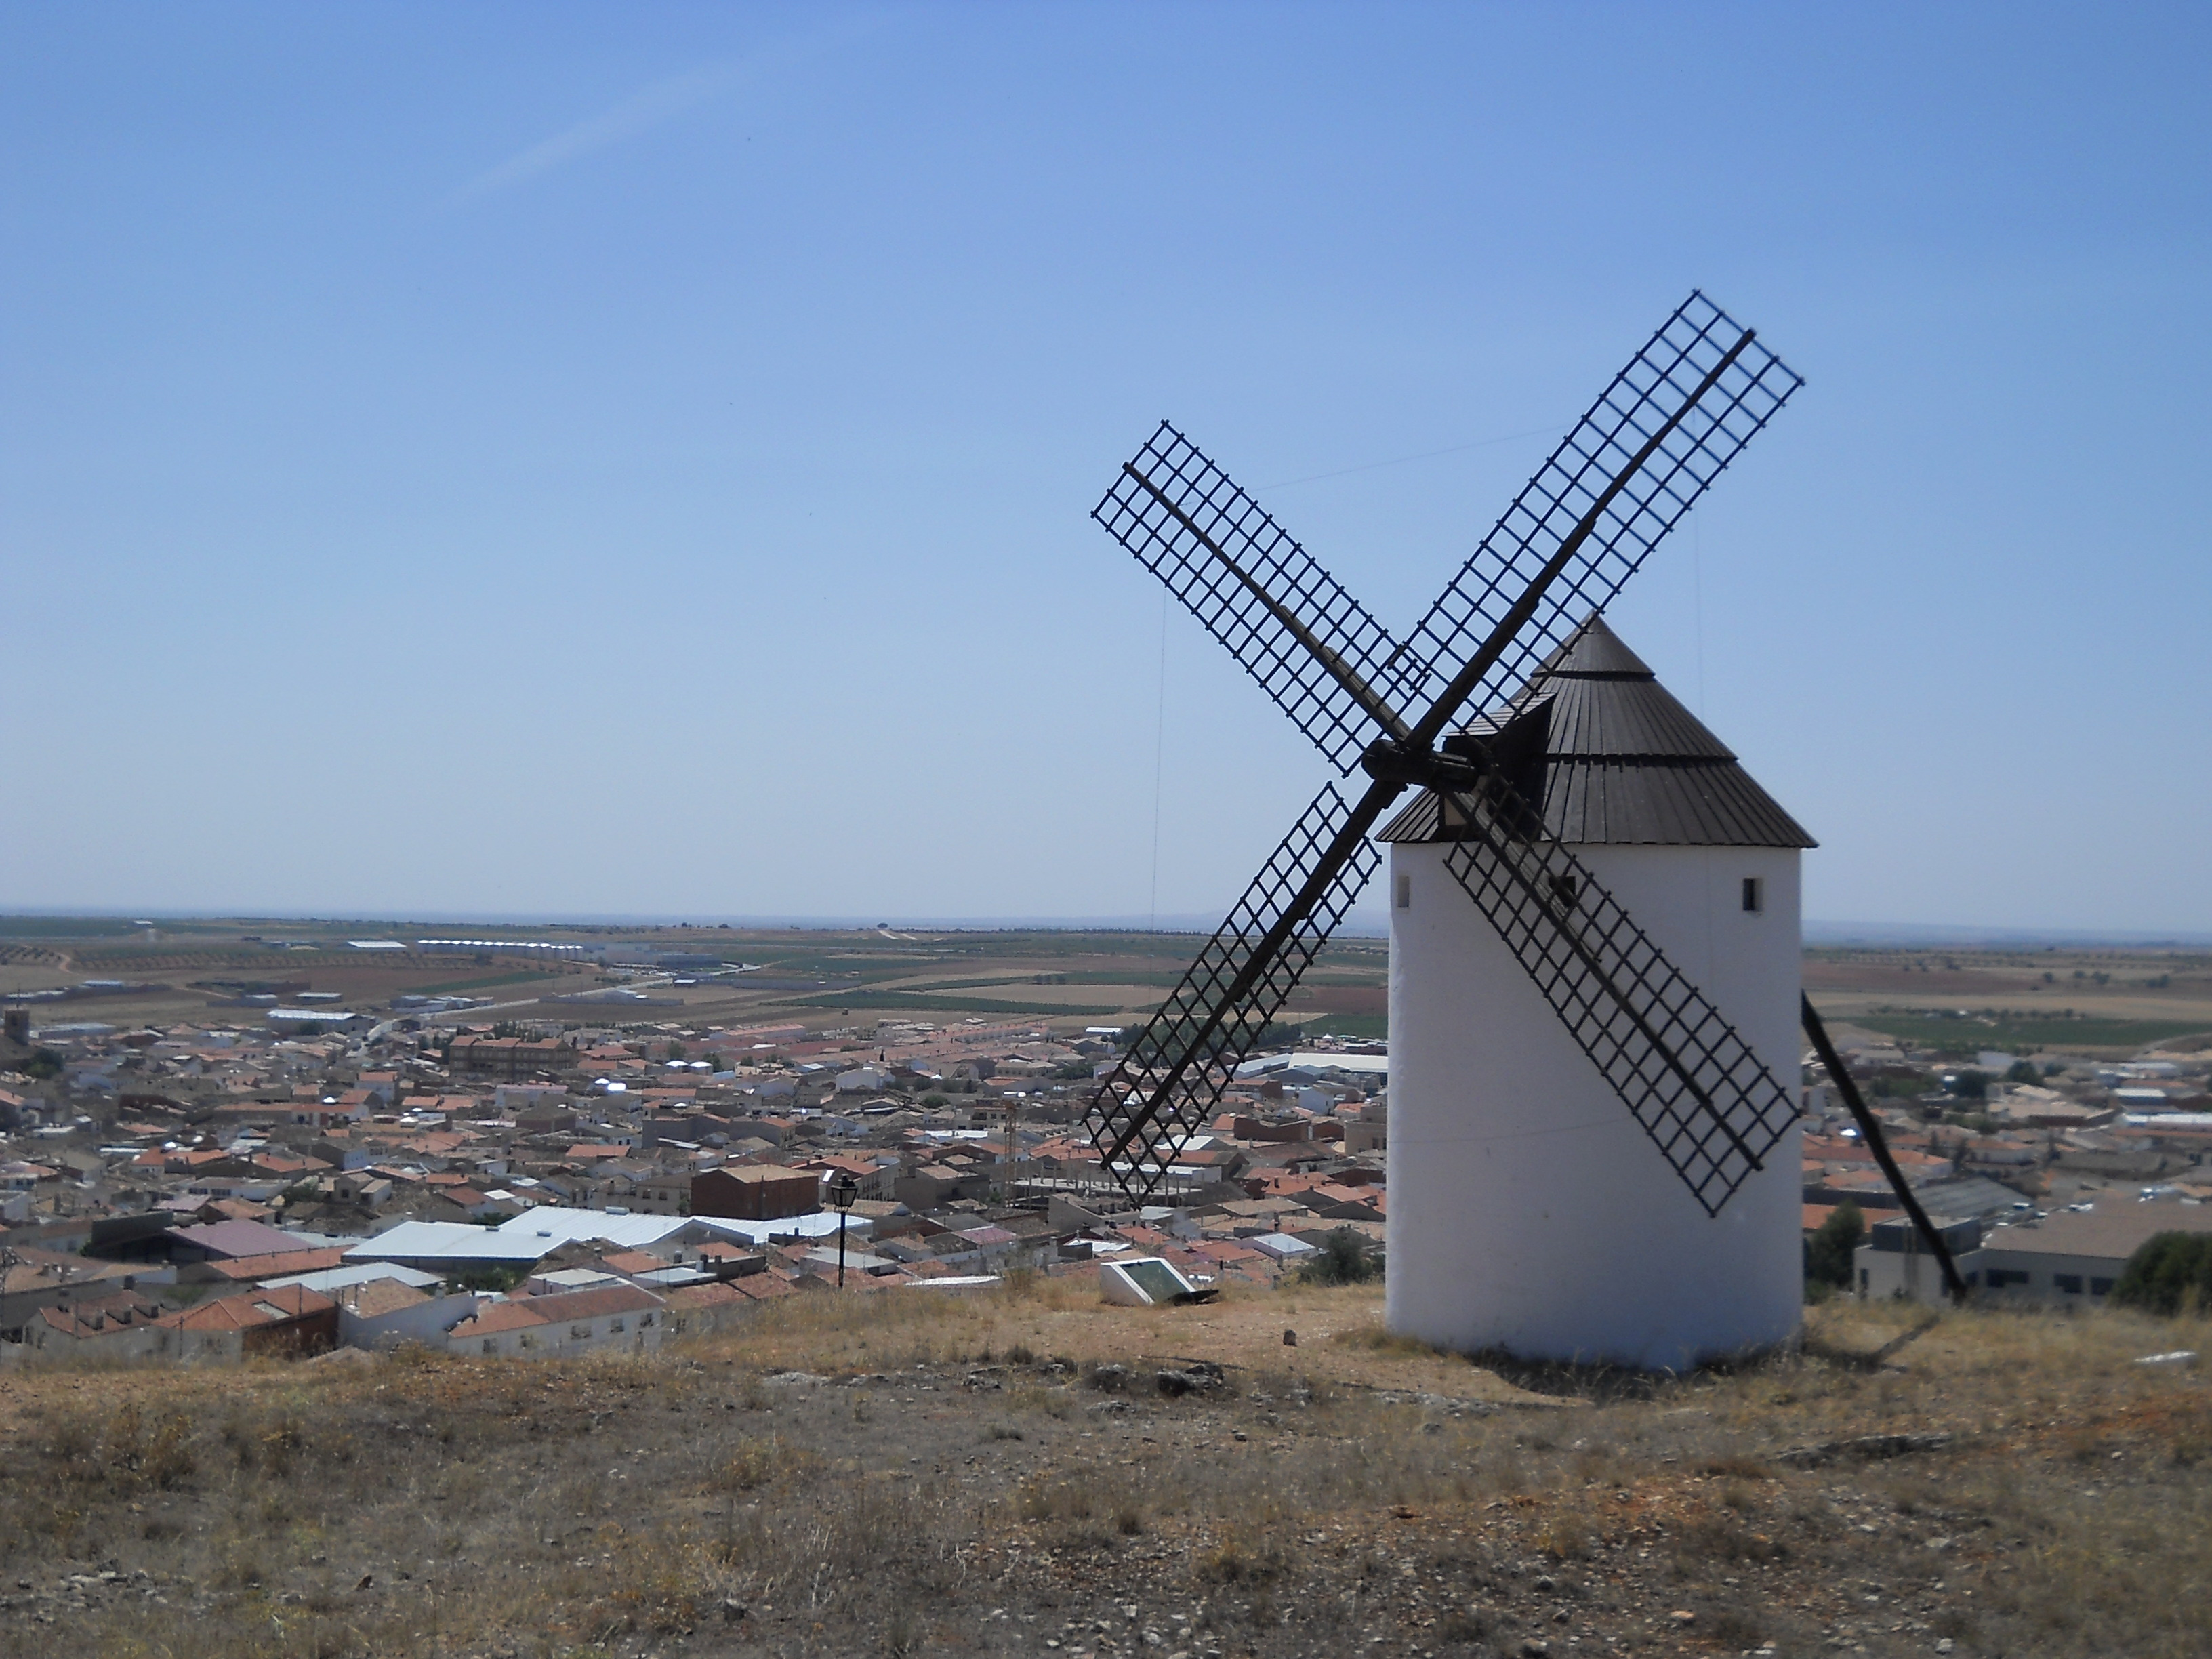
\includegraphics[width=0.45\textwidth]{img/molino.jpg}
	\caption{Distinguir el molino del pueblo del fondo no es difícil para un humano aunque sí para una máquina.}
	\label{img:ejemplomolino}
\end{figure}

\REV{pq es importante el problema de la segmentación} Autores como González y Woods en \cite{lib:gonzalez} enuncian el problema de ``segmentación de imágenes no triviales como una de las tareas más dificiles en el procesamiento de imágenes''. En este sentido, insisten en que ``la exactitud de la segmentación determina el éxito o error de los procesos de análisis computerizados''. Otros autores \cite{lib:sonka} hablan de la sementación como una ``técnica en al que se divide la imagen en partes que tienen una correlación con objetos o áreas del mundo real contenidas en la imagen''. Definido formalmente:

\begin{definition}\label{def:definicionproblema}
Dada una imagen $Q$ que se pude subdividir en $n$ regiones $R_{1}, \dots, R_{n}$, y sabemos que $P$ es una cierta propiedad booleana que cumplen todos los píxeles de la región $R_{i}, \forall  i=1,\dots ,n$, se deberá cumplir siempre que:
\begin{enumerate}
	\item $\bigcup_{i=1}^{n}R_{i}=Q$;
	\item En una región $R_{i}, \forall i=1,\dots ,n$ todos sus píxeles están conectados;
	\item $R_{i}\cap R_{j}=\emptyset, \forall i, j : i\neq j;$
	\item $P(R_{i}) = \text{ VERDADERO }, \forall  i=1,\dots ,n;$
	\item $P(R_{i}\cup R_{j}) = \text{ FALSO }, \forall  i=1,\dots ,n.$
\end{enumerate}
\end{definition}

En conclusión, en este proceso se lleva a cabo la división de la imagen en regiones donde cada una (desde 2 hasta $n$, este número dependerá del problema que estemos resolviendo) harán mención al fondo y a cada objeto. Además, todas las regiones serán independientes entre sí, esto es, un pixel pertenecerá solamente a la región $i$ cuando hablemos de segmentación completa. Centrando el problema únicamente en aquellas imágenes en escala de grises, nuestra pretensión será obtener aquellas regiones que contienen a un objeto centrándonos en sus tonalidades, esto es, por medio de técnicas de umbralización \REV{seguro?}.


% 1.3. SOLUCIÓN
\section{Solución propuesta}\label{sec:solucion}
\REV{Nosotros vamos a utilizar técnicas difusas, para empezar. ¿Por qué? (Incertidumebre en torno a los píxeles, péridda de información captación imágenes,...)}

Existen tres técnicas para poder llevar a cabo la segmentación de una imagen:
\REV{explicación y referencia}
\begin{enumerate}[label=\alph*)]
	\item Segmentación basada en umbralización.
	\item Técnicas basada en agrupamiento de píxeles en regiones.
	\item Técnicas basadas en la detección de bordes.
\end{enumerate}

En este trabajo se va a centrar la segmentación por medio de las técnicas de umbralización. Para ello lo que tendremos que hacer será calcular los umbrales que separen las regiones que se hayan encontrado, de forma que situaremos las regiones entre un umbral $t_{i}$ y uno $t_{i+1}$. Para ejemplificar esto, tomaremos la umbralización binaria en la cual se dispondrá de un único umbral $t$. De esta forma, todos los elementos de la imagen que se encuentren por encima del umbral pertenecerán a una región  y los que estén por debajo a la segunda. Esta técnica se basa únicamente en detectar los diferentes tonos de gris de la imagen, así que mirando el histograma de la imagen (fig. \ref{img:rice}, podríamos ver cómo existe una frontera entre la intensidad $t=71$ y el resto creando diferencias en los niveles de gris. \cite{art:refbarrenechea}

\begin{figure}
\centering
	\subfloat{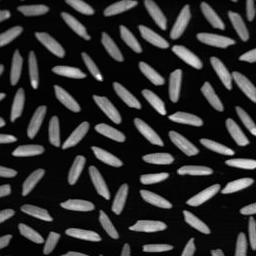
\includegraphics[width=0.3\textwidth]{img/rice}}
	\subfloat{
\includegraphics[width=0.3\textwidth]{img/umbra-rice}}\\
	\subfloat{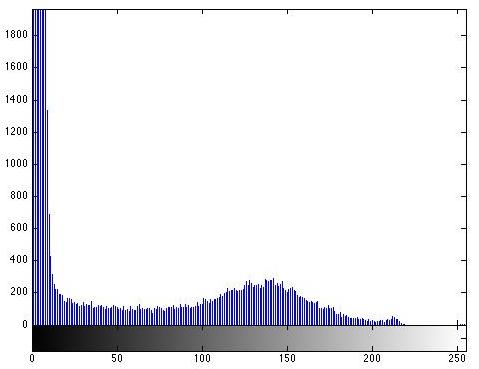
\includegraphics[width=0.4\textwidth]{img/hist-rice}}
	\caption{(a) Imagen original. (b) Imagen segmentada. (c) Histograma de la imagen original. Se puede ver que en t=71 se produce un mínimo con respecto a los otros niveles de gris y que por eso se escoge como umbral.}
	\label{img:rice}
\end{figure}


\REV{solución al pq...} Se debe tener en cuenta que la umbralización es un método rápido y de coste computacional bajo por lo que se puede realizar en tiempo real. Como sólo basa su algorítmica en el histograma de la imagen hace que sea una método sencillo e intuitivo aunque esto también hace que tenga problemas ante el ruido y objetos o fondos que no sean uniformes.

La solución que se presenta en este trabajor se haya por medio de lógica difusa. Se han utilizado funciones REF, de Dombi, de agregación y penalti. En el capítulo \ref{basicos} se hace mención a todos estos conceptos y se explican poníendose en práctica a partir del capítulo \ref{monoumbral}. En el capítulo \ref{cap:conclusiones} se presentan todas las conclusiones obtenidas así como las líneas de trabajo futuro.

%La umbralización es rápida, de coste computacional bajo y se puede realizar en tiempo real.
%Sencilla e intuitiva.
%Técnica útili si el fondo y los objetos son uniformes.
%Problemas: el ruido, niveles de gris similares entre obejto y fondo, solapamientos de objetos...
%La obtención de un umbral se basará en el histograma de la imagen. No se considera la información espacial.

% 1.4. REELEVANCIA
\section{Reelevancia}\label{sec:reelevancia}

En el campo de la medicina \cite{lib:suri} se ha experimentado una mejora sustancial en la efectividad de las pruebas médicas gracias a diferentes opciones como los rayos X, la tomografía computerizada, la resonancia magnética, la tomografía por emisión de positrones (PET), imágenes de ultrasonidos y otras. La revolución digital y el gran poder de procesamiento que disponen los ordenadores ha conseguido que los profesionales comprendan la compleja anatomía humana, aunque esto no ha sido suficiente ya que se ha visto necesario poder obtener los bordes, las superficies y la segmentación de los órganos. Estos órganos segmentados y sus bordes son clave para poder conseguir que un especialista médico pueda hacer una cirugía adecuada para muchas ramas de la medicina, debido a la importancia de tener datos en tiempo real. \REV{[Insertar figura que vaya con esto].}


Pruebas médicas
Localización de tumores y otras patologías
Medida de volúmenes de tejido
Cirugía guiada por ordenador
Diagnóstico
Planificación del tratamiento
Estudio de la estructura anatómica

Análisis automático de detección de errores.

Sensor de huella digital
Localización de objetos en imágenes de satélite (teledetección).
\REV{Alargar esto}


% 1.5. OBJETIVOS
\section{Propósito y objetivos}\label{sec:objetivos}

Este proyecto se centra en estudiar técnicas de segmentación para un único umbral y la generalización de estas en múltiples umbrales en imágenes en blanco y negro e intentar mejorar las técnicas de las que actualmente se disponen intentando generalizarlas de forma que los parámetros no dependan del problema. 

Además, para poder conseguir el propósito anterior se estipularon los siguiente objetivos:
\begin{itemize}
	\item Investigar y conocer técnicas actuales de segmentación de imagen de forma que estas sean el punto de partida.
	\item Analizar y evaluar las funciones que J. Dombi propone en \cite{art:dombi}. Comparar estas con las funciones REF y sustituirlas en la construcción de los conjuntos difusos para conocer sus efectos.
	\item Implementar diferentes algoritmos de segmentación con el conocimiento adquirido anteriormente evaluando su mejora y haciendo las correcciones necesarias con la intención de generalizar el método de forma máxima.
	\item Implementar diferentes algoritmos que incluyan la agregación de las diferentes funciones estudiadas para la segmentación en los puntos anteriores comprobando si esto mejora los resultados anteriores.
	\item Analizar todos los puntos anteriores a fin de concluir los resultados del trabajo así como dirimir si se ha podido conseguir cumplir el propósito inicial.
\end{itemize}

%1.6 ANÁLISIS BIBLIOGRÁFICO
\section{Análisis bibliográfico}
No tengo claro aun que poner aquí. Próximamente.

\chapter{Conceptos básicos}\label{preliminares}\label{basicos}

Este capítulo pretende ser una introducción a todos los conceptos teóricos necesarios para la correcta comprensión del trabajo que se detalla en esta memoria. 


\section{Procesamiento digital de imagen}\label{sec:procesamiento}
Un imagen $Q$ puede ser entendida como una función de dos variables, $q(x,y)$, donde $x$ e $y$ son las coordenadas en el plano de cada elemento (píxel) y la función da como resultado el nivel de gris o intensidad asociada a ese píxel. En concreto, cuando $x$ e $y$ así como la intensidad $q(x,y)$ son finitas y discretas hablaremos de que tenemos una imagen digital. Por eso mismo, el procesamiento digital de imagen se puede definir como aquel que se hace con imágenes digitales a través de un ordenador. Tiene su origen con la introducción de las primeras imágenes digitales a principios de 1920, donde se enviaban imágenes entre Londres y Nueva York por medio de un cable submarino.

Es claro que los seres humanos disponemos del sentido de la vista como el sentido más desarrollado para interacturar con el medio, pero esta está limitada a la banda visible dentro del espectro electromagnético. En cambio, el procesamiento digital de imagen puede cubrir el análisis de todo el espectro electromagnético, lo que incluye los ultrasonidos, el infrarrojos, rayos X, etc. Esta es la principal razón por la que el procesamiento digital de imagen puede incluirse en una gran cantidad de campos.\REV{quitar ultima frase?}

Dentro del procesamiento de imagenes digitales se encuentra la visión artificial. Esta es una subcampo de la inteligencia artificial (IA) y pretende emular la visión humana, incluyendo la capacidad de aprender así como el manejo directo de imágenes como datos de entrada a un problema dado. Actualmente, este campo está poco desarrollado \cite{lib:gonzalez} ya que el avance está siendo mucho más lento de lo que se esperaba en un primer momento. El análisis de imagen, que pretende entender cómo está formada la imagen, está situada a caballo entre la visión artificial y el procesamiento de imágen, y será lo que utilizaremos en este trabajo.

No hay una clara frontera entre el procesamiento de imagen y la visión artificial, esto hace que se hable de un paradigma que incluye 3 tipos de procesos; de bajo nivel, medio nivel y alto nivel. Dentro del nivel bajo se pueden incluir todos los procesos primitivos que tienen como objetivo reducir el ruido, realzar el contraste o ajustar la nitidez, por ejemplo. En un segundo nivel, más avanzado, se encuentran todos los procesos que tienen como entrada una imagen y obtienen atributos de esta. Pueden ser procesos como la segmentación (que se tratará aquí), descripción de objetos de la imagen o recocimiento de los mismos. En el último nivel se encuentran todas aquellas técnicas que hacen que todo ``tenga sentido'' ya que hacen que el análisis imite a la forma cognitiva de la mente humana.


\subsection{Imágenes digitales}\label{sec:imagenesdigitales}
Como ya se ha explicado en el apartado anterior, se habla de imagen digital cuando se puede ser capaz de determinar todos sus elementos (píxeles), es decir, estos son de forma finita y discreta. A partir de esta idea, se dispone de dos formas de representación para las imágenes en niveles de gris, en los rangos $[0,1]\in\RR$ y $[0,255]\in\NN$. En el primer caso diremos que la imagen está normalizada. Además, las imágenes digitales serán representadas por una matriz que contendrá cada uno de sus píxeles de manera ordenada.


\begin{figure}
\centering
    \subfigure[Niveles de gris]
    {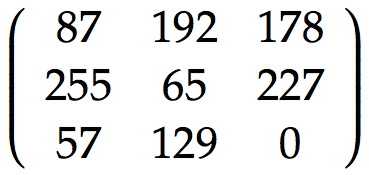
\includegraphics[height=0.1\textwidth]{img/matriznivelesgris.jpg}}\quad
    \subfigure[Normalizada]
    {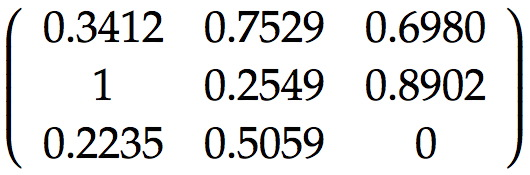
\includegraphics[height=0.1\textwidth]{img/matriznormalizada.jpg}}\quad\ 
    \subfigure[Gráfica]
    {
\includegraphics[width=0.1\textwidth]{img/imagendigital.jpg}}
    \caption{Imagen digital en diferentes representaciones.}
    \label{fig:defimagen}
\end{figure}

Como se puede apreciar en la figura \ref{fig:defimagen} cuanto más cercano a 0 sea el número, más negro será el nivel de gris, y cuanto más cercano a 1 ó 255, más blanco. En el caso de imágenes en color, se utiliza el formato RGB ({\em Red}, {\em Green} y {\em Blue}) donde existe una matriz como las anteriores por cada uno de los colores y al superponerlas se obtiene la imagen que vemos habitualmente.

\begin{definition}\label{def:histograma}
Se define el histograma de una imagen $Q$ con niveles de gris en el intervalo [0, 255] como la función $h(q) = n_q$ donde $n_q$ es el número de píxeles en la imagen con la intensidad $q$.
\end{definition}

Un ejemplo gráfico de la función de histograma para una imagen puede encontrarse en la figura \ref{img:rice}.


\subsection{Herramienta para el procesamiento digital: \MATLAB}\label{sec:matlab}
\MATLAB\ (abreviatura de {\em Matrix Laboratory}) es una herramienta de software matemático que ofrece un lenguaje de programación (lenguaje M) y un entorno de desarrollo integrado. Fue creado en 1984 por el informático y matemático Cleve Moler el cual buscaba una forma alternativa de ejecutar programas de álgebra en {\em Fortran}.

Entre sus prestaciones básicas están la manipulación de matrices, la representación de datos y funciones o la implementación de algoritmos así como la creación de interfaces de usuario (GUI). Además, el paquete básico de \MATLAB\ puede ser expandido por medio de {\em toolboxes}, como es el caso de este trabajo, donde se utilizará la relativa  a procesamiento de imagen. Se puede disponer también del software {\em Simulink} para trabajar conjuntamente a \MATLAB.

\subsection{Contraste}
Como en el trabajo se hace uso de imágenes con alto y bajo contraste, disponer una pequeña explicación. Pillar de los libros del laboratorio. \REV{Revisar}.

\subsection{Ruido en las imagenes}\label{sec:ruido}
Se condidera que una imagen está degradada cuando tiene ruido, esto es, cuando tiene defectos con respecto a la imagen original (fig. \ref{fig:defruido}). La principal fuente de ruido en images digitales se da en la adquisición o transmisión de las imagenes. Esto se puede deber a las condiciones ambientales o a la calidad de los sensores durante la toma de la imagen. Por ejemplo, la luminosidad, el polvo en el ambiente, etc. pueden ser determinantes. Por otra parte, en el caso de la transmisión, las imágenes pueden ser corrompidas por interferencias en el medio de transmisión, principalmente. Esto es claro cuando se transmite una imagen de un satélite, ya que la atmósfera interferir y provocar que la imagen recibida en la base terráquea no sea exactamente igual.
\begin{figure}
\centering
    \subfigure[Imagen original]
    {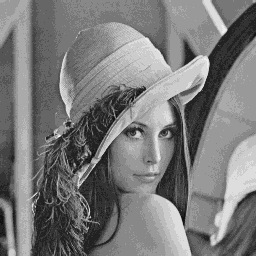
\includegraphics[width=0.3\textwidth]{img/lena}}\quad
    \subfigure[Imagen con ruido `sal y \mbox{pimienta}']
    {
\includegraphics[width=0.3\textwidth]{img/lenas&p}}\quad
    \subfigure[Imagen con ruido gausiano]
    {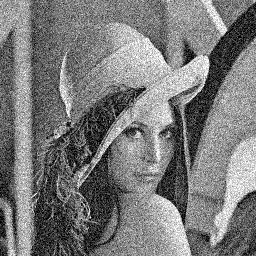
\includegraphics[width=0.3\textwidth]{img/lenaga}}
    \caption{Imagen de Lena con diferentes tipo de ruido}
    \label{fig:defruido}
\end{figure}

Las imágenes con ruido también se pueden crear artificialmente. Para ello utilizamos una cierta función $H$ de degradación, a la que añadimos un ruido al que llamaremos $\eta$ de forma que obtendremos una nueva imagen $g(x,y)$ que tendrá una serie de imperfecciones. Todo el ruido creado de esta forma se aplicará directamente sobre los píxeles de la imagen lo que provocará cambios en su histograma en una forma u otra. Aun así, debemos tener en cuenta que no hay relación directa entre la intensidad nueva que tienen los píxeles y la anterior. 

Existen muchos tipos de ruido como el exponencial, el gamma, el uniforme, etc. pero en esta memoria se han utilizado, el gausiano y el de tipo impulsivo o de `sal y pimienta'.

\subsubsection{Ruido gausiano}
Este puede ser uno de los modelos de ruido más utilizado en la práctica debido a que tiene una gran maleabilidad matemática. Basa su forma de actuar sobre la imagen en la función gausiana de probabilidad:
$$p(z) = \frac{1}{\sqrt{1}{2\pi\sigma}} e^\frac{-(z-\mu)^2}{2\sigma^2}$$
donde $z$ representa la intensidad, $\mu$ la media de $z$ y $\sigma$ la desviación estándar. Este tipo de ruido puede crearse en \MATLAB\ a través de la función \mintinline{matlab}{imnoise(img_var, 'gaussian')} sabiendo que \mintinline{matlab}{img_var} es la variable donde está almacenada la imagen en tipo \mintinline{matlab}{uint8}.

\subsubsection{Ruido de tipo `sal y pimienta'}
Este tipo de ruido, formalmente llamado impulsivo, hace que se conviertan píxeles de forma aleatoria en píxeles con intensidad 0 y 255. Esta es la razón de su particular nombre. De nuevo, fijándonos en \MATLAB, podremos crear imágenes con este tipo de ruido por medio del comando \mintinline{matlab}{imnoise(img_var, 'salt & pepper', prob_val)}, de nuevo \mintinline{matlab}{img_var} es la variable donde se almacena la imagen y \mintinline{matlab}{prob_val} es un valor entre 0 y 1 que hace las veces de probabilidad de la aparición del ruido. 

En este trabajo, se han utilizado imágenes con ruido para comprobar la adecuación o no de los algoritmos de segmentación al ruido. Ejemplos de ambos tipos de ruido se han presentado en la figura \ref{fig:defruido}.


% LOGICA DIFUSA
\section{Lógica difusa}\label{sec:logicadifusa}
La lógica difusa fue introducida por el matemático L. A. Zadeh \cite{art:zadeh} en 1965 con la intención de poder extender la lógica clásica o {\em crips} de forma que permitiera manejar y procesar la información que se compone de términos inexactos, imprecisos o subjetivos. Es, al fin y al cabo, un intento de imitar la forma de deducción del cerebro humano para trasladarlo a las máquinas. Se comenzará recordando la lógica clásica para después extender los conceptos a la difusa.

En primer lugar, definiremos el universo finito, $U$,  con el que se  trabajará, de forma que contenga todos aquellos elementos con los que se desee trabajar, esto es, $U = \{u_{1}, u_{2}, \dots, u_{n}\}$. En la lógica clásica simplemente asignamos verdadero o falso a cada uno de los elementos del conjunto que se estudia. Por esta razón, al definir un conjunto $A$ podremos decir que este contiene o no a los elementos del universo $U$ con una certeza absoluta. De esta manera, daremos un valor de 1 cuando $u_{i}$ esté incluido en $A$ (verdadero) y un valor de 0 cuando no lo esté (falso). En esta última idea se refleja por medio de la función de pertenencia al conjunto  $A$, $\mu_{A}$ (ecuación \ref{eq:logicaclasica}).
\begin{equation}\label{eq:logicaclasica}
\begin{aligned} 
	A = \{(u_{i}, \mu_{A}(u_{i})) | u_{i}\in U\}\\
	\mu_{A}:U\rightarrow \{0,1\} \text{ tal que}\\
	\mu_{A}(u) = \left\{ \begin{aligned}
		1 \quad\text{si}\quad u\in A\\
		0 \quad\text{si}\quad u\notin A
 	\end{aligned}\right.
\end{aligned}
\end{equation}
%\REV{revisar ecuación con respecto al ejemplo} Se da más adelante la concreta.

 Podemos considerar el problema de determinar si una persona es alta o no. Para la lógica clásica, este razonamiento se simplificará en buscar un valor a partir del cual podamos definir que cierta persona es alta. Para el siguiente ejemplo, tomaremos 1,75 metros como referencia, donde $A$ es el conjunto de las personas altas. De este modo, $\mu_{A}=1 \text{ si } u>1,75$ y en otro caso $\mu_{A}=0$. En la figura \ref{fig:altoclasica} se puede ver la representación del concepto `alto' para las posibles alturas que se pueden presentar.

\subfile{graficos/logicaclasicagraf}

Por otra parte, la lógica difusa dispone de la función de pertenencia más compleja, lo que nos hace poder decir que alguien es `poco alto' o `bastante alto' ya que no daremos un par de valores ($\{0,1\}$) sino cualquiera de los contenidos en el intervalo que definen. Así $\mu_{A}$ será una función que asigna un valor entre 0 y 1 a cada elemento de $A$.\begin{equation}\label{eq:logicadifusa}
\begin{aligned} 
	A = \{(u_{i}, \mu_{A}(u_{i})) | u_{i}\in U\}\\
	\mu_{A}:U\rightarrow [0,1]
\end{aligned}
\end{equation}                
Si continuamos con el ejemplo se verá que el conjunto alto ($A$) esta vez se define como explica la ecuación \ref{eq:ejemplodifusa}. 

\begin{equation}\label{eq:ejemplodifusa}                
	\mu_{A}(u) = \left\{ \begin{aligned}
		1 \quad&\text{si}\quad u\geq 2\\
		2u - 3 \quad&\text{si}\quad 1.5>u>2\\
		0 \quad&\text{si}\quad u\leq 1.5
 	\end{aligned}\right.
 \end{equation}           
Esta nueva función de pertenencia hace que podamos distinguir 3 zonas dentro de su representación (figura \ref{fig:altodifusa}). Se tendrá de nuevo la etiqueta `alto' y `no alto' que hacen que su pertenencia sea certera. Se dispondrá, también, una parte de la pertenencia a la que llamaremos `difuso' donde el conjunto no afirma ser ni `alto' ni `no alto' sino que está en una situación intermedia. En este caso se habla de que el elemento $a_{i}$ que se encuentra ahí pertenece a $A$ con grado $\mu_{A}(a_{i})$.
                
\subfile{graficos/logicadifusagraf}

Más formalmente, denotaremos al conjunto que incluye a todos los conjuntos difusos como $\FF(u)$ a todos aquellos que se encuentran definidos sobre un referencial finito ($|U| = n$) por lo que $U$ no será un conjunto vacío.
 


% FUNCIONES REF
\section{Funciones de equivalencia restringida (REF)}\label{sec:ref}
El concepto de función de equivalencia restringida (REF por sus siglas en inglés) surge del concepto de equivalencia y el de similitud \cite{art:refbarrenechea}. Este concepto es muy utilizado para la comparación de imágenes y su intención es dar una medida de cómo de iguales o similares son dos elementos $x$ e $y$. Para poder definir el concepto de REF, necesitamos varios previamente. 

\begin{definition}\label{def:negacionestricta}
Una negación estricta es aquella función $c : [0, 1] \rightarrow [0, 1]$ que cumple que $c(0)=1$ y $c(1)=0$ y es estrictamente decreciente y continua. Además, si $c$ es involutiva se considera que se habla de una negación fuerte.
\end{definition}

\begin{definition}\label{def:automorfismo}
Llamaremos automorfismo ($\varphi$) a todas aquellas funciones del intervalo unidad tal que $\varphi : [0, 1] \rightarrow [0, 1]$ sean continuas y estrictamente crecientes propiciando que $\varphi(0)=0$ y $\varphi(1)=1$.
\end{definition}

En 1979, E. Trillas \cite{art:thtrillas} enunció el siguiente teorema. 
\begin{theorem}[Teorema de Trillas]\label{th:trillas}
Una función $c : [0, 1] \rightarrow [0, 1]$ es una negación fuerte si, y sólo si, existe un automorfismo del intervalo unidad tal que $c(x)=\varphi^{-1}(1-\varphi(x))$.
\end{theorem}

\begin{definition}\label{def:ref}
Una función $REF  : [0, 1] \rightarrow [0, 1]$ es llamada de equivalencia restringida cuando cumple que:
	\begin{enumerate}
	\item $REF(x, y) = REF(y, x), \forall x, y \in [0, 1];$
	\item $REF(x, y) = 1$, si y sólo si, $x=y$;
	\item $REF(x, y) = 0$, si y sólo si, $x=1$ e $y=0$ ó si $x=0$ e $y=1$;
	\item $REF(x, y) = REF(c(x), c(y)),  \forall x, y \in [0, 1]$, siendo $c$ una negación fuerte.
	\item $\forall x, y, z \in [0, 1]$, si $x\leq y\leq z$, entonces $REF(x, y)\geq REF(x, z)$ y  $REF(y, z)\leq REF(x, z)$
	\end{enumerate}
\end{definition}

\begin{proposition}\label{prop:contruccionref}
Sean dos automorfismos $\varphi_{1}$ y $\varphi_{2}$, se llamará función $REF$ a la construcción que cumpla que: 
$$REF(x,y) = \varphi_1^{-1}(1-|\varphi_2(x)-\varphi_2(y)|) \quad\text{con}\quad c(x) = \varphi_2^{-1}(1-\varphi_2(x)).$$ 
Además, si tenemos una $REF$ y un automorfismo en $\unitinterval$, la aplicación de estos ($F=\varphi \circ REF$) es otra $REF$.
\end{proposition}

\begin{theorem}\label{th:ref}
Una función continua $REF:\unitinterval^2 \rightarrow\unitinterval$ que cumpla que $REF(1,x)=x, \xinunitinterval$, es una función $REF$ asociada con la función $I:\unitinterval^2\rightarrow\unitinterval$ con $I$ continua y asociativa si y sólo si existe un automorfismo $\varphi$ en $\unitinterval$ tal que:
$$REF(x,y)=\varphi^{-1}(1-\abs{(\varphi(x)-\varphi(y))})\quad\text{ y }\quad c(x)=\varphi^{-1}(1-\varphi(x))$$
\end{theorem}

%\REV{Teorema que hace que estos automorfismos puedan ser 1 solo?} No lo pongo pq no lo utilizo.


% FUNCIONES DE AGREGACIÓN
\section{Funciones de agregación}\label{sec:agregacion}
%\REV{funciones de agregación vs operadores de agregación ¿Qué es más correco para nombrarlos?} -> Funciones de agregación.
Las funciones de agregación tienen como propósito reducir las dimensiones de la información a partir de la combinación de los datos de entrada obteniendo una salida que los represente \cite{art:montero, art:calvoagregacion}. Su aplicación se extiende en muchos casos prácticos y teóricos como la lógica multievaluada, control difuso, la toma de decisión, etc \cite{art:paternain}.  Se definirá una función de agregación como sigue:

\begin{definition}\label{def:agregacion}
Se dice que $M : \unitinterval^n \rightarrow \unitinterval$ es una función de agregación de dimensión $n$ siempre que satisfaga:
	\begin{enumerate}
	\item $M(x_1, \dots, x_n) = 0$ si y sólo si $x_1=\dots=x_n=0$;
	\item $M(x_1, \dots, x_n) = 1$ si y sólo si $x_1=\dots=x_n=1$;
	\item $M$ es una función estrictamente creciente.
	\end{enumerate}
\end{definition}
\begin{definition}
Una función de agregación $M$ será llamada media si
$$ \min(x_{1}, \dots, x_{n})  \leq M(x_{1}, \dots, x_{n}) \leq \max(x_{1}, \dots, x_{n}).$$
\end{definition}

En este proyecto se utilizarán mayoritariamente las funciones de agregación idempotentes, esto es, que cumplen que $M(x,\dots ,x)=x, \forall x$. En particular, una función de agregación idempotente es una media. Entre las funciones que utilizaremos encontramos la media aritmética, el mínimo, el máximo o la media geométrica. Además, se definen a continuación otras que no son de uso tan común.
% OWA
\subsection{Funciones OWA}
En esta sección se introduce el concepto de las funciones de media ponderada ordenada (OWA, {\em  ordered weighted averaging}) \cite{art:yagerowa, art:paternain, art:bustinceowa}. Se basan en la idea de generar una media, ordenando primero los elementos a agregar, para luego darles mayor relevancia a una parte de ellos. Este tipo de función generaliza la media aritmética, siendo esta el OWA en el que todos los elementos del vector de pesos son iguales.

\begin{definition}\label{def:owa}
Una  función $F:\unitinterval^n\rightarrow\unitinterval$ será una función OWA de dimensión $n$ si existe un vector $w=(w_{1},w_{2},\dots,w_{n})\in \unitinterval^{n}$ tal que $\sum_{i}w_{i}=1$ de forma que
$$F(x_{1},\dots,x_{n})=\sum^{n}_{j=1}w_{j}x_{\sigma(j)}$$
donde $x_{\sigma(j)}$ es el $j$-ésimo mayor elemento del vector $(x_{1},\dots,x_{n})$.
\end{definition}

Por tanto para poder obtener un resultado adecuado, deberá utilizarse un vector de pesos $w$ que se adecúe a las necesidades del problema. En este trabajo se emplea la versión `al menos la mitad' %\REV{nombre}. Solucionado.
 que tiene como vector de pesos aquel que se obtiene con la ecuación \ref{eq:pesosowamayoria}. Esto generará una agregación donde destaquen todos aquellos elementos que se encuentren por detras de la mediana.
% a $w=(w_{1}\dots w_{i}, w_{i+1}\dots w_{n})$ sabiendo que $\abs{1, \dots, i}=\abs{i+1,\dots,n}$ de forma que $w_{j}=\frac{1}{2n}$ si $1\leq j\leq i$ y $w_{j}=0$ en el resto de los casos.\REV{buscar la versión buena, esto es sólo para los cardinales pares}.\REV{volver a redactar. Incluir construcción.}

\begin{equation}\label{eq:pesosowamayoria}
	 w_i = Q\left(\frac{i}{t+1}\right) - Q\left(\frac{i+1}{t+1}\right), \forall i\in \{1, \dots, n\}, \text{   sabiendo que}
\end{equation}
	 $$Q(r) = \left\{\begin{aligned}
	 	0 					&\quad \text{si}\quad r<0,5\\
	 	\frac{r-0,5}{0,5}	&\quad \text{si}\quad 0,5\leq r\leq 1\\
	 	1 					&\quad \text{si}\quad r>1\\
	\end{aligned}\right.$$
\REV{forma ecuación}

%\REV{reescrito}
Además, en la segunda parte del estudio, se emplea el OWA `la mayoría de'. Este OWA pretende destacar aquellos elementos que son mayores en el vector $x$. Esto se hace realidad por medio de un vector de pesos donde son nulos los pesos relativos a aquellas $x_i$ más pequeñas. Para la construcción del vector de pesos, se utilizará, también, la ecuación \ref{eq:pesosowamayoria}



% CHOQUET
\subsection{Integral Choquet}
Para este otro tipo de función \cite{art:choquet, art:sugenochoquet} de agregación se pretende dar una nueva de forma de representar un conjunto de datos en una única salida. De esta forma, se define primeramente una medida a través de la cual se calculará la forma en la que cada elemento del conjunto de datos tendrá reelevancia en la agregación final. Para ello definimos el concepto de medida difusa.
\begin{definition}\label{def:medidadifusa}
Dado $U$ un universo finito; $\mathcal{P}(U)$ el conjunto de todos los subcojuntos de $U$. Una medida difusa es una función $\mu:\mathcal{P}(U)\rightarrow\unitinterval$ que satisface que:
\begin{enumerate}
	\item $\mu(\emptyset)=0$ y $\mu(U)=1$.
	\item $A\subseteq B \Rightarrow \mu(A)\leq\mu (B), \forall A, B \subseteq U$.
\end{enumerate}
\end{definition}

A continuación definimos la función integral Choquet conociendo que tomaremos su versión discreta por el contexto en el que se está trabajando.

\begin{definition}\label{def:choquet}
Dado un vector $(x_1,\dots,x_n)$, sea $\sigma$ una permutación de $\{1,...,n\}$ tal que $x_{\sigma(j)}$ es el $j$-ésimo mayor elemento del vector $(x_{1},\dots,x_{n})$. La integral discreta de Choquet con respecto a la medida difusa $\mu$ es 
$$Ch_{\mu}(x)=\sum_{i=1}^{n}x_{\sigma(i)}(\mu(\{\sigma(i),\dots,\sigma(n)\})-\mu(\{\sigma(i+1),\dots,\sigma(n)\}))$$
tomando la convención de que $\{\sigma(n+1),\sigma(n)\}=\emptyset$.
\end{definition}

\begin{proposition}\label{prop:choque2owa}
Si denotamos a $w_{\sigma, i}^{\mu} = \mu(\{\sigma(i),\dots,\sigma(n)\})-\mu(\{\sigma(i+1),\dots,\sigma(n)\})$ se obtiene la siguiente definición de la integral Choquet en función de los operadores OWA definidos en \ref{def:owa}:
$$\sum_{i=1}^{n} w_{\sigma, i}^{\mu} \cdot x_{\sigma(i)}.$$
\end{proposition}


% FUNCIONES DE SIMILITUD
\section{Funciones de similitud}\label{sec:similitud}
El concepto de similitud \cite{art:fan1, art:fan2} surge cuando queremos medir cómo de parecidos son dos conjuntos difusos. Este concepto es muy parecido al de REF, pero en este caso se consideran conjuntos y no elementos. Por esta razón, utilizamos las REF como base para definir las funciones de similitud.
\begin{definition}\label{def:similitud}
Dada una función $M$ de agregación (definición \ref{def:agregacion}) y una función $REF$ (definión \ref{def:ref}) llamaremos a $SM$ función de similitud si $SM : \FF(X) \times \FF(X) \rightarrow [0,1]$ está definida tal que 
$$SM(A,B)=M^n_{i=1}REF(\mu_A(x_i), \mu_B(x_i))$$
y satisface las siguientes condiciones:
	\begin{enumerate}
	\item $SM(A, B) = SM(B, A), \forall A, B \in \FF(X)$;
	\item $SM(A, A_c) = 0$, si y sólo si A no es difuso;
	\item $SM(A, B) = 1$ si y sólo si A = B;
	\item Si $A\leq B\leq C$, entonces $SM(A, B)\geq SM(A,C)$ y $SM(C, B)\geq SM(C,A)$;
	\item $SM(A_c, B_c) = SM(A,B)$
	\end{enumerate}	
\end{definition}

\begin{remark}\label{obs:funcionesref}
Durante el desarrollo de este trabajo se buscará la similitud entre conjuntos difusos y el conjunto $\tilda1$. Se define el conjunto $\tilda1 =\{(u_{i}, \mu_{\tilda1}(x)=1)|u_{i}\in U \}$, esto es, aquel en el que todos sus elementos tienen pertenencia absoluta.
\end{remark}


% FUNCIONES PENALTI
\section{Funciones penalti}\label{sec:penalti}
Una función penalti  \cite{art:calvo} es una función de agregación, por lo que dispone de un vector de entradas del que devuelve un único resultado. Si todos los elementos del vector son iguales, entonces, claramente, la salida será eso mismo. Ahora bien, el problema surge cuando hay algún elemento diferente ya que en ese momento la idea será buscar una salida todo lo parecida posible a la entrada. En este sentido, es elemento o elementos diferentes tendrán una cierta discrepancia con los demás y justamente esto es lo que se pretende minimizar, la discrepancia, para dar una salida adecuada. 

\begin{definition}\label{def:penalti}
La función $P:[a,b]^{n+1}\rightarrow \RR^{+} = [0, \infty]$ es una función penalti si y sólo si satiface que:
\begin{enumerate}
	\item $P(x, y) \geq 0, \forall x, y$
	\item $P(x, y) = 0$ si $x_{i}=y \forall i=1,\dots ,n$
	\item $P(x,y)$ es cuasiconvexa en $y$ para cualquier $x$, esto es, $P(x, \lambda\cdot y_{1} +(1-\lambda)\cdot y_{2})\leq \max(P(x, y_{1}), P(x, y_{2}))$.
\end{enumerate}
\end{definition}
La función en la que se basan las penalti es $$f(x)=\arg\min_{y} P(x,y)$$ si $y$ es el único mínimo e $y=\frac{a+b}{2}$ si el conjunto de minimizadores es el intervalo $(a, b)$.

\begin{theorem}
Todas las funciones de agregación llamadas medias pueden ser escritas como una función basada en una función penalti expresada en la definición \ref{def:penalti}.
\end{theorem}


% FUNCIONES DE DOMBI
\section{Funciones de Dombi}\label{sec:dombi}
Las funciones de Dombi \cite{art:dombi} son operadores de equivalencia con una definición diferente a las REF presentadas en la sección \ref{sec:ref}. Con esta relación lo que se pretende conocer es como de iguales son dos elementos de un conjunto difuso dado, pero aplicando nuevas ideas para la construcción del resultado. 
%\REV{Definición completa?} Pues así se va a quedar.
\begin{definition}\label{def:dombi}
Dados $x=(x_1, x_2, \dots,x_n)$ y $w=(w_1,w_2,\dots,w_n)$, denotaremos $D$ como una función de equivalencia de Dombi cuando tengamos que 
$$D(w,x)=\frac{1}{2}\left(1+\prod(1-2x_{i})^{w_{i}}\right)$$
\end{definition}
\begin{lemma}\label{def:propiedadesdombi}
La función de equivalencia de Dombi, $D$, cumple las siguientes propiedades:
\begin{enumerate}
	\item $D:\unitinterval\times\unitspace \text{ es continua}$;
	\item $D((w_1,w_2),(0,0)) = 1$;\quad$D((w_1,w_2),(1,1)) = 1$;
	\item $D((w_1,w_2),(0,1)) = 0$;\quad$D((w_1,w_2),(1,0)) = 0$;
	\item $D((w_1,w_2),(x,c(x))) = 0$.
\end{enumerate}
\end{lemma}
%\REV{propiedades}



%NOTACIÓN
\section{Notación}\label{sec:notacion}

A lo largo del trabajo se asumirá la notación que sigue para estos conceptos.

\begin{description}
    \item[Imagen]: la denotaremos con $Q$.
    \item[Coordenadas de un pixel]: $(x,y)$.
    \item[Máximo nivel de gris]: $L$.
    \item[Número de filas de $Q$]: $N$.
    \item[Número de columnas de $Q$]: $M$.
    \item[Intensidad de un pixel]: $q(x,y)$ de forma que $0\leq q(x,y)\leq L-1, \forall (x,y)\in Q$.  
    \item[Histograma]: $h(q)$. Función para conocer el número de pixeles con la intensidad $q$. 
    \item[Media de una imagen]:$$m_Q=\frac{\sum_{q=0}^{L-1}qh(q)}{\sum_{q=0}^{L-1}h(q)}$$
    \item[Área de una imagen]: $$A(Q) = \sum_{q=0}^{L-1} q h(q)$$
\end{description}


\chapter{Segmentación de imágenes con un solo umbral con funciones de Dombi}\label{monoumbral}

En este capítulo en primer lugar se presentarán todas las herramientas algorítmicas que se van a utilizar para llevar a cabo los experimentos de este trabajo, haciendo énfasis en la forma de utilización para funciones de Dombi. Seguidamente se mostarán los resultados obtenidos para la segmentación monoumbral con estas funciones.


\section{Métodos algorítmicos de segmentación de un único umbral}\label{sec:algoritmosmono}
\documentclass[main]{subfiles}

\begin{document}

% ALGORITMO 1 GENERAL
\subsection{Algoritmo general maximizando la similitud}

Este algoritmo, que se presenta en \cite{art:barrenechea}, pretende conseguir obtener un único umbral a partir de la maximización de la similitud.

\begin{algorithm}
\begin{algorithmic}[1]
\REQUIRE Una imagen $Q$ en escala de grises donde sus píxeles estén entre $0$ y $L-1$.
\ENSURE El umbral $t$ a partir del cual se divide $Q$ en objeto y fondo.
\FOR {$t$:=0 hasta $L-1$}
\STATE Divisón de la imagen en dos clases $C_b(t)$ y $C_o(t)$. Para cada una de estas clases, calcular su media: $m_b(t)$ y $m_o(t)$.
\STATE Construcción del conjunto difuso $Q_t$.
\STATE Calcular la $SM(\tilda1, Q_t)$. \label{lin:alg1:similitud}
\ENDFOR
\RETURN \{$t$ | max($SM$)\}
\end{algorithmic}
\caption{Maximización de la similitud}\label{alg:algoritmo1}
\end{algorithm}

En el algoritmo anterior se necesitan varias definiciones que se explican a continuación. En primer lugar, se describe el método de creación de los conjuntos difusos para lo que se explica previamente el cálculo de las medias para el fondo y el objeto.

\begin{definition}\label{def:mediasmonoumbral}
Teniendo en cuenta la definición de la media de una imagen que se ha dado en el apartado \ref{sec:notacion}, y disponiendo del histograma de la imagen $h(q)$ para un cierto nivel $q, \forall q\in Q$, se define la media de los píxeles del fondo como:
$$m_b(t)=\frac{\sum_{q=0}^{t}qh(q)}{\sum_{q=0}^{t}h(q)};$$
y para los píxeles del objeto como:
$$m_o(t)=\frac{\sum_{q=t+1}^{L-1}qh(q)}{\sum_{q=t+1}^{L-1}h(q)}.$$
\end{definition}

\begin{definition}\label{def:conjuntodifusomonoumbral}
Dada $Q$, una imagen en la escala de L niveles de gris, y $t$, un nivel de gris de forma que $0\leq t\leq L-1$. Teniendo en cuenta que $F$ es una función $REF$ ya que la $REF \circ \varphi$ lo es, se define el conjunto
$$Q_t = \{(q, \mu_{Q_t}(q)|q\in \{0,1,\dots, L-1\}\}$$
teniendo en cuenta que
$$\mu_{Q_t}(q) = \left\{ \begin{aligned}
    F \left(\frac{q}{L-1}, \frac{m_b(t)}{L-1} \right) = \varphi\left(REF\left(\frac{q}{L-1}, \frac{m_b(t)}{L-1} \right)\right) & \quad\text{si}\ q\leq t,\\
    F \left(\frac{q}{L-1}, \frac{m_o(t)}{L-1} \right) = \varphi\left(REF\left(\frac{q}{L-1}, \frac{m_o(t)}{L-1} \right)\right) & \quad\text{si}\ q> t.
 \end{aligned}\right.$$
 \end{definition}

\begin{remark}
Como parece lógico a la vista de la definición \ref{def:conjuntodifusomonoumbral}, es necesario poder enumerar aquellas funciones que se utilizarán como $REF$ y como automorfismo $\varphi$. Para todos los casos se tendrá $\varphi = x$ y, además, se distinguirán las siguientes funciones $REF$:
\begin{enumerate}
    \item $REF(x,y)=1-\abs{x-y}$
    \item $REF(x,y)=1-\abs{x-y}^2$
    \item $REF(x,y)=1-\abs{x-y}^{0.5}$
    \item $REF(x,y)=(1-\abs{x-y})^2$
    \item $REF(x,y)=(1-\abs{x-y})^{0.5}$
\end{enumerate}
\end{remark}

Debido a la formulación de este tarbajo, se sustituirá la aplicación anterior que actúa como función $F$ en la definición \ref{def:conjuntodifusomonoumbral} por la función de Dombi \cite{art:dombi} definidas en \ref{def:dombi}. De esta forma, en este caso, los conjuntos difusos quedarán como explica la ecuación \ref{eq:conjdifusosdombimono}.
\begin{equation} \label{eq:conjdifusosdombimono}
    \mu_{Q_t}(q) = \left\{ \begin{aligned}
        F \left(w,\left(\frac{q}{L-1}, \frac{m_b(t)}{L-1}\right)\right) = \frac{1}{2}\left(1 + \left(1-2\frac{q}{L-1}\right)^w\cdot\left(1-2\frac{m_b(t)}{L-1}\right)^w\right)& \quad\text{si}\ q\leq t,\\
        F \left(w,\left(\frac{q}{L-1}, \frac{m_o(t)}{L-1}\right)\right) = \frac{1}{2}\left(1 + \left(1-2\frac{q}{L-1}\right)^w\cdot\left(1-2\frac{m_o(t)}{L-1}\right)^w\right)& \quad\text{si}\ q> t.
     \end{aligned}\right.
\end{equation}
%\REV{Está bien definido cómo he metido el parámetro d??}
Además, el último paso del bucle, en la línea \ref{lin:alg1:similitud} (Algoritmo \ref{alg:algoritmo1}=, se lleva a cabo la busqueda de la similitud frente al conjunto $\tilda1$. Para poder llevar a cabo este cálculo, tal y como se especifica en la definición \ref{def:similitud}, necesitamos utilizar una función $REF$, que será $REF_2=1-\abs{x-y}^2$, y la agregación $M$, la media aritmética ($M=\frac{i=1}{n}\sum_1^n x_i$). De esta forma, quedará como sigue:
\begin{equation}\label{eq:similitud}
    SM(\tilda1, Q_{t}) = M^{L-1}_{q=0}(h(q)\cdot REF_2(1,\mu_{Q_t}(q)))
\end{equation}


% ALGORITMO DEL ÁREA
\subsection{Algoritmo del área}

Este algoritmo, que se presenta en \cite{art:barrenechea} también, pretende hayar un nuevo umbral a través de la creación de una función $REF$, tal y como se explica en el teorema \ref{prop:contruccionref}.

\begin{algorithm}
\begin{algorithmic}[1]
\REQUIRE Una imagen $Q$ en escala de grises donde sus píxeles estén entre $0$ y $L-1$.
\ENSURE El umbral $t$ a partir del cual se divide $Q$ en objeto y fondo.
\FOR {$t$:=0 hasta $L-1$}
\STATE \begin{equation*}\begin{split}
A(Q_t)= \sum_{q=0}^{t} h(q)\varphi_1^{-1}\left(1-\abs{\varphi_2\left(\frac{q}{L-1}\right)-\varphi_2\left(\frac{m_b(t)}{L-1}\right)}\right) + \\ \sum_{q=t+1}^{L-1} h(q)\varphi_1^{-1}\left(1-\abs{\varphi_2\left(\frac{q}{L-1}\right)-\varphi_2\left(\frac{m_o(t)}{L-1}\right)}\right)
\end{split}\end{equation*}
\ENDFOR
\RETURN \{$t$ | max($A(Q_t)$)\}
\end{algorithmic}
\caption{Umbralización del área}\label{alg:algoritmo2}
\end{algorithm}

Esta es, realmente, una nueva versión del algoritmo de maximización de similitud anterior. Por esta razón, se prepara una formulación para conocer la relación de la similitud en función del área ($A$) que se ha calculado. Se intentará, por tanto, simplificarlo retirando la función de similitud $SM$.
\begin{proposition}
Dada una agregación $M$, la media aritmética, y la función $REF_2$, una función de equivalencia restringida formada según la definición \ref{def:ref}. Si se construyen dos conjuntos difusos $Q_{t_1}$ y $Q_{t_2}$ de acuerdo a definición \ref{def:conjuntodifusomonoumbral} de la imagen $Q$. Si disponemos de una medida de similitud presentada en \ref{def:similitud} podemos afirmar que:
$$SM(\tilda1, Q_{t_1})\leq SM(\tilda1, Q_{t_1})\quad \text{si y sólo si}\quad A(Q_{t_1})\leq A(Q_{t_1})$$
\end{proposition}
\begin{proof}
Sabiendo que $REF(1,x)=x, \xinunitinterval$, entonces:
$$SM(\tilda1, Q_{t_1})
= \frac{1}{\sum_{q=0}^{L-1}h(q)}\sum_{q=0}^{L-1}\left( h(q)REF_2(1, \mu_{Q_{t_1}}(q))\right)
= \frac{1}{\sum_{q=0}^{L-1}h(q)}\sum_{q=0}^{L-1}\left( h(q)\mu_{Q_{t_1}}(q)\right)
= \frac{A(Q_{t_1})}{\sum_{q=0}^{L-1}h(q)}.$$
Por esta razón, también se podrá decir que $SM(\tilda1, Q_{t_2}) = \frac{A(Q_{t_2})}{\sum_{q=0}^{L-1}h(q)}$ lo que prueba la proposición anterior.
\end{proof}

En este algoritmo, se utilizan 3 pares de automorfismos para darle forma al área.

%\begin{table}[h!]\begin{center}
%\resizebox*{14cm}{!}{\begin{tabular}{c||c|c||c}
%&$\varphi_1$ & $\varphi_2$ & $A(Q_t)$\\\hline\hline
%(1)&$x$ & $x$ & $\sum_{q=0}^{L-1} h(q) - \left(\sum_{q=0}^{t} \left(1-\abs{\frac{q}{L-1}-\frac{m_b(t)}{L-1}}\right) - \sum_{q=t+1}^{L-1} \left(1-\abs{\frac{q}{L-1}-\frac{m_o(t)}{L-1}}\right)\right)$ \\\hline
%(2)&$x^d$ & $x$ & $\sum_{q=0}^{t} h(q) \left(1-\abs{\frac{q}{L-1}-\frac{m_b(t)}{L-1}}\right) - \sum_{q=t+1}^{L-1} h(q) \left(1-\abs{(\frac{q}{L-1}-\frac{m_o(t)}{L-1}}\right)$ \\\hline

%(3)&$x^1-(1-x)^{1/2}$ & $x$ & $\sum_{q=0}^{L-1} h(q) - \left(\sum_{q=0}^{L-1} h(q) \left(\frac{q}{L-1}-\frac{m_b(t)}{L-1}\right)^2 - \sum_{q=t+1}^{L-1} h(q) \left(\frac{q}{L-1}-\frac{m_o(t)}{L-1}\right)^2\right)$ \\\hline

%\end{tabular}}\end{center}
%\caption{Porcentajes de acierto para los diferentes \datasets y configuraciones para {\em train}.\label{resultTrain}}
%\end{table}

\begin{enumerate}\label{enum:funcionesalg2}
    \item Se toma $\varphi_1(x) = \varphi_2(x) = x, \xinunitinterval$.
    $$A(Q_t) = sum_{q=0}^{L-1} h(q) - \left(\sum_{q=0}^{t} \left(1-\abs{\frac{q}{L-1}-\frac{m_b(t)}{L-1}}\right) - \sum_{q=t+1}^{L-1} \left(1-\abs{\frac{q}{L-1}-\frac{m_o(t)}{L-1}}\right)\right)$$
    \item Se toma $\varphi_1(x) = x^d \text{ con } d\neq0, \xinunitinterval \text{ y } \varphi_2(x)=x, \xinunitinterval$.
    $$\sum_{q=0}^{t} h(q) \left(1-\abs{\frac{q}{L-1}-\frac{m_b(t)}{L-1}}\right) - \sum_{q=t+1}^{L-1} h(q) \left(1-\abs{\frac{q}{L-1}-\frac{m_o(t)}{L-1}}\right)$$
    \item Se toma $\varphi_1(x) = 1-\sqrt{1-x}, \xinunitinterval \text{ y } \varphi_2(x)=x,\xinunitinterval$
    $$\sum_{q=0}^{L-1} h(q) - \left(\sum_{q=0}^{L-1} h(q) \left(\frac{q}{L-1}-\frac{m_b(t)}{L-1}\right)^2 - \sum_{q=t+1}^{L-1} h(q) \left(\frac{q}{L-1}-\frac{m_o(t)}{L-1}\right)^2\right)$$
\end{enumerate}
En total, se dispondrá de 4 versiones diferentes. Se debe tener en cuenta que en la en el par (2) de automorfismos se dispondrá de $d=0,5$ y $d=2$.

% ALGORITMO 3
\subsection{Algoritmo de selección del umbral óptimo}\label{sec:algoritmo3}

\begin{definition}\label{def:conjuntoHmonoumbral}
Dada $Q$, una imagen en la escala de L niveles de gris, y $t$, un nivel de gris de forma que $0\leq t\leq L-1$, se calcula su conjunto $H(Q_t)$ como
$$H(Q_t) = \{(q, \mu_{H(Q_t)}(q)|q\in \{0,1,\dots, L-1\}\}$$
teniendo en cuenta que
$$\mu_{Q_t}(q) = \left\{ \begin{aligned}
    \frac{m_b(t)}{L-1} & \quad\text{si}\ q\leq t,\\
    \frac{m_o(t)}{L-1} & \quad\text{si}\ q> t.
 \end{aligned}\right.$$
 \end{definition}

En el algoritmo, necesitaremos, después, calcular la similitud que existe entre el conjunto $Q_t$ y el conjunto $H(Q_t)$. Para ello aplicamos la definición \ref{def:similitud}:
$$SM(Q_t, H(Q_t)) = M^{L-1}_{q=0}(h(q)REF(\mu_{Q_t}(q), \mu_{H(Q_t)}(q)))$$
Tendremos en cuenta que $M$ seguirá siendo la media aritmética y $REF=1-\abs{x-y}^2 \xinunitinterval$. Si a través de la uniformidad simplificamos la expresión anterior, obtendremos:
$$SM(Q_t, H(Q_t)) = \frac{1}{\sum_{q=0}^{L-1}h(q)} \sum_{q=0}^{L-1}\left(h(q)(1-(\mu_{Q_t}(q)-\mu_H{(Q_t)}(q))^2)\right)$$

\begin{algorithm}[!ht]
\begin{algorithmic}[1]
\REQUIRE Una imagen $Q$ en escala de grises donde sus píxeles estén entre $0$ y $L-1$.
\ENSURE El umbral óptimo $t^*$ a partir del cual se divide $Q$ en objeto y fondo.
\FOR {$t$:=0 hasta $L-1$}
\STATE Calcular los conjuntos $Q_t$ como se describe en la definición \ref{def:conjuntodifusomonoumbral}.
\STATE Calcular los conjuntos $H$ como se muestra en la definición \ref{def:conjuntoHmonoumbral}.
\STATE Calcular la $SM(Q_t, H(Q_t))$.
\ENDFOR
\RETURN \{$t*$ | max($SM$)\}
\end{algorithmic}
\caption{Selección del umbral óptimo}\label{alg:algoritmo3}
\end{algorithm}



%ALGORITMO GLOBAL
\subsection{Otros algoritmos}\label{sec:otrosalgoritmos}
\subsubsection{Algoritmo de umbralización global}\label{sec:algoritmoglobal}

Entre los algoritmos que se encargan de segmentar la imagen con un único umbral, este es el más simple aunque en ocasiones podemos obtener resultados suficientemente buenos según que aplicación queramos darle.

\begin{algorithm}[!ht]
\begin{algorithmic}[1]
\REQUIRE Una imagen $Q$ en escala de grises donde sus píxeles estén entre $0$ y $L-1$.
\ENSURE El umbral óptimo $t$ a partir del cual se divide $Q$ en objeto y fondo.
\STATE $t = 128$;
\COMMENT{Se selecciona un umbral inicial cualquiera, aquí se tomará el valor medio de los posibles}
\REPEAT
\STATE $tant = t$;
\STATE $G1 = \{(x, y) | q(x, y) > t0\}$
\STATE $G2 = \{(x, y) | q(x, y) \leq t0\}$
\STATE $m1 = \frac{1}{\abs{G1}} \sum_{i\in G1} i$
\STATE $m2 = \frac{1}{\abs{G2}} \sum_{i\in G2} i$
\STATE $t = \frac{m1+m2}{2}$
\UNTIL {$\abs{tant-t} < \varepsilon$}
\COMMENT {El valor $\varepsilon$ es un cierto error dispuesto por el programador.}
\RETURN $t$
\end{algorithmic}
\caption{Umbralización global.}\label{alg:global}
\end{algorithm}

En este sentido, para el buen funcionamiento del algoritmo es necesario que la imagen tenga una clara separación entre el objeto y el fondo, expresada con un valle en el histograma de la imagen. Se debe tener cuidado al elegir el parámetro $\varepsilon$ ya que de él depende el número de iteraciones del bucle. Normalmente, conforme este crece, menor es el número de iteraciones necesarias para un resultado adecuado.


% ALGORTIMO DE OTSU
\subsubsection{Algoritmo de Otsu}\label{sec:algoritmootsu}

El algoritmo de Otsu \cite{art:otsu} basa su técnica de umbralización, también, en el histograma de la imagen que recibe. Para ello, trata las probabilidades que se le ortorgan a cada uno de los niveles de gris de los que dispone la imagen. Si tomamos una imagen $Q$ que tenga sus intensidades entre $[1, 2, \dots, L]$, podremos expresar la probablidad de cada intensidad como
$$p_i = \frac{n_i}{N}, \quad p_i \geq 0\quad\text{ sabiendo que }\quad\sum_{i=0}^{L-1}p_i=1$$
siendo $n_i$ el número de píxeles de intensidad $i$ y $N$ el número total de píxeles en la imagen $Q$.

Ahora, supondremos que podemos clasificar los elementos de la imagen en dos clases, $C_0$ y $C_1$ que tendrán a los píxeles $[0,\dots,k]$ y $[k+1,\dots,L-1]$ respectivamente. Definirán su probabilidad como
$$\omega_0 = \Pr(C_0) = \sum_{i=0}^{t}p_i=\omega_0(t)\qquad\text{y}\qquad
\omega_1 = \Pr(C_1) = \sum_{i=t+1}^{L-1}p_i=\omega_1(t)$$
y su media como
$$\mu_0=\sum_{i=0}^t i \Pr(i|C_0) = \sum_{i=0}^t \frac{ip_i}{\omega_0} = \frac{\mu(t)}{\omega(t)}\qquad\text{y}\qquad
\mu_1=\sum_{i=t+1}^{L-1} i \Pr(i|C_1) = \sum_{i=t+1}^{L-1} \frac{ip_i}{\omega_1} = \frac{\mu_T-\mu(t)}{1-\omega(t)}$$
donde
$$\omega(k)\sum_{i=0}^k ip_i   \qquad\text{y}\qquad   \mu(k)=\sum_{i=0}^k ip_i$$

Por último, se puede definir
$$\mu_T = \mu(L-1) = \sum_{i=0}^{L-1} ip_i$$
y todas estas definiciones podemos asegurar que cumplirán que
$$\omega_0\mu_0+\omega_1\mu_1 = \mu_T   \qquad\text{y}\qquad   \omega_0+\omega_1 = 1$$
Con la intención de evaluar lo adecuado o no que es cada umbral $t$, podemos definir la varianza de cada uno como
$$\sigma_B^2(t) = \omega_0(\mu_0-\mu_T)^2 + \omega_1(\mu_1-\mu_T)^2 = \omega_0\omega_1(\mu_1-\mu_0)^2$$
Con todo ello, para encontrar el umbral óptimo $t^*$ sólo deberemos encontrar aquella varianza que maximice a las demás.
$$\sigma_B^2(t^*) = \max_{1\leq k <L}\left\{\sigma_B^2(t)\right\}$$

Al resumir todo lo anterior en lenguaje algorítmico se encuentra:
%\REV{El umbral de 1..L en vez de 0..L-1} Solucionado, se queda igual que todos de 0..L

\begin{algorithm}
\begin{algorithmic}[1]
\REQUIRE Una imagen $Q$ en escala de grises donde sus píxeles estén entre $0$ y $L-1$.
\ENSURE El umbral óptimo $t^*$ a partir del cual se divide $Q$ en objeto y fondo.
\FOR {$t$:=0 hasta $L-1$}
\STATE $\omega_0$(t) = $\sum_{i=1}^{t}p_i$
\STATE $\mu_0$(t) = $\sum_{i=1}^t \frac{ip_i}{\omega_0}$
\STATE $\omega_1$(t) = $\sum_{i=t+1}^{L}p_i$
\STATE $\mu_1$(t) = $\sum_{i=t+1}^L \frac{ip_i}{\omega_1}$
\STATE $\sigma_B^2(t) = \omega_0\omega_1(\mu_1-\mu_0)^2$
\ENDFOR
\RETURN \{$t^*$ | $max_t(\sigma_B^2$)\}
\end{algorithmic}
\caption{Selección del umbral óptimo según Otsu.}\label{alg:otsu}
\end{algorithm}


% ALGORITMO DE LA ENTROPÍA DE RENYI
\subsubsection{Algoritmo de maximización de la entropía de Renyi}\label{sec:algoritmorenyi}
Este algoritmo, enunciado en \cite{art:sahoo}, busca el umbral óptimo de la imagen a través de la maximización de la entropía que se produce en la imagen definida por Renyi. Al igual que en el algoritmo de Otsu se empieza definiendo dos clases, la correspondiente al fondo y la del objeto. Para cada una de ellas se define su probabilidad
$$p(C_0)=\sum_{i=0}^{t}p_i\qquad\text{y}\qquad p(C_1)=\sum_{i=t+1}^{L-1}p_i$$
donde con ambas probabilidades se cumple que $p(C_0)+p(C_1)=1$.

%Método de el anterior KAPUT
%$$H_T=-\sum_{i=0}^{L-1} p_i \ln p_i$$
%$$H_{C_0}(t)=-\sum_{i=0}^{t} \frac{p_i}{p(C_0)} \ln \frac{p_i}{p(C_0)}$$
%$$H_{C_1}(t)=-\sum_{i=t+1}^{L-1} \frac{p_i}{p(C_1)} \ln \frac{p_i}{p(C_1)}$$
%$$p(C_0)\sum_{i=0}^{t}p_i$$
%$$p(C_1)\sum_{i=0}^{t}p_i$$
%$$p(C_0)+p(C_1)=1$$

%$$C_0:\frac{p_0}{p(C_0)},\frac{p_1}{p(C_0)},\dots,\frac{p_t}{p(C_0)}$$
%$$C_1:\frac{p_0}{p(C_1)},\frac{p_1}{p(C_1)},\dots,\frac{p_t}{p(C_1)}$$
%$$H_{T}^{\alpha}(t) = \frac{1}{1-\alpha}\ln \sum_{i=0}^{L-1}\left(p_i\right)^\alpha \quad\text{con }\alpha\neq 1$$
A continuación se define la entropía para ambas clases sabiendo que $\alpha\neq 1$.
$$H_{C_0}^{\alpha}(t) = \frac{1}{1-\alpha}\ln \sum_{i=0}^{t}\left(\frac{p_i}{p(C_0)}\right)^\alpha \qquad\text{y}\qquad
H_{C_1}^{\alpha}(t) = \frac{1}{1-\alpha}\ln \sum_{i=t}^{L-1}\left(\frac{p_i}{p(C_1)}\right)^\alpha$$

Llegado este punto, se puede encontrar el umbral óptimo $t^*(\alpha)$ aquel que maximice la suma de las entropías de las clases:
$$t^*(\alpha)=\max_{0\leq t<L}\left\{H_{C_0}^{\alpha}(t)+H_{C_1}^{\alpha}(t)\right\}.$$

Por medio de experimentación se ha comprobado que el umbral anterior no es igual para todos los valores de $\alpha$. Este hecho se formaliza de la siguiente forma:
$$t^*(\alpha)=\left\{\begin{aligned}
    t^*_1 & \text{  si  }0<\alpha<1,\\
    t^*_2 & \text{  si  }\alpha\rightarrow1,\\
    t^*_3 & \text{  si  }1<\alpha<\infty.
\end{aligned}\right.$$

Por esta razón, se hace necesario emcontrar un umbral $t$ que no sea dependiente de $\alpha$. Para ello se deben calcular un umbral para cada una de las 3 situaciones enumeradas y ordenarlos de mayor a menor, algo que simbolizaremos como $\tonee\leq\ttwo\leq\tthree$. De estas forma, definiremos el umbral óptimo de la imagen como
$$t^*_c = t_{(1)} \left(p(t_{(1)})+\frac{1}{4}\omega\beta_1\right)
        + \frac{1}{4}t_{(2)}\omega\beta_2
        + t_{(3)} \left(1-p(t_{(3)})+\frac{1}{4}\omega\beta_3\right)$$
en donde tendremos en cuenta que $p(t)=\sum_{i=1}^t(p_i)$ y $\omega=p(t_{(3)})-p(t_{(1)})$ además del vector $(\beta_1, \beta_2, \beta_3)$ que se toma así:
$$(\beta_1, \beta_2, \beta_3) =  \left\{\begin{aligned}
    (1, 2, 1) & \quad\text{si} &\abs{\tonee-\ttwo}\leq 5 \text{ y } \abs{\ttwo-\tthree}\leq 5,\\
    (1, 2, 1) & \quad\text{si} &\abs{\tonee-\ttwo}  >  5 \text{ y } \abs{\ttwo-\tthree}  >  5,\\
    (0, 1, 3) & \quad\text{si} &\abs{\tonee-\ttwo}\leq 5 \text{ y } \abs{\ttwo-\tthree}  >  5,\\
    (3, 1, 0) & \quad\text{si} &\abs{\tonee-\ttwo}  >  5 \text{ y } \abs{\ttwo-\tthree}\leq 5,
\end{aligned}\right.$$

En definitiva, el umbral $t^*_c$ puede verse como una media ponderada de los valores de $t_1^*, t^*_2, t^*_3$ por lo que se puede afirmar
$$\min\{t_1^*, t^*_2, t^*_3 \}\leq t_c^* \leq\max\{t_1^*, t^*_2, t^*_3\} = \tonee \leq t_c^* \leq \tthree$$
esta agregación consigue evitar los malos resultados que podrían darse si no se utilizara un parámetro $\alpha$ correcto al igual que integra todas las características de la imagen.

\begin{algorithm}
\begin{algorithmic}[1]
\REQUIRE Una imagen $Q$ en escala de grises donde sus píxeles estén entre $0$ y $L-1$.
\ENSURE El umbral óptimo $t*$ a partir del cual se divide $Q$ en objeto y fondo.

\STATE $\alpha = [0.3, 0.99999, 10]$
\STATE \COMMENT{Para facilitar la implementación, se tendrá en cuenta únicamente un alfa de cada uno de los casos, cuando se estabilizan cada uno de los casos}
\FOR {$\alpha_i \in \alpha$}
    \STATE $H_T=0$
\FOR {$t'=0$ hasta $L-1$}
        \STATE $p_{C_0} = \sum_{i=0}^{t'}p_i$
        \STATE $p_{C_1} = \sum_{i=t'+1}^{L-1}p_i$
        \STATE $H_{C_0}^{\alpha}(t') = \frac{1}{1-\alpha}\ln \sum_{i=0}^{t'}\left(\frac{p_i}{p(C_0)}\right)^\alpha$
        \STATE $H_{C_1}^{\alpha}(t') = \frac{1}{1-\alpha}\ln \sum_{i=t'}^{L-1}\left(\frac{p_i}{p(C_1)}\right)^\alpha$
        \STATE $H_T(t') = H_T(t') + H_{C_0} +H_{C_1}$
     \ENDFOR
    \STATE $t_{mejor}(i) = \max_{0\leq j<L}\left\{H_T(j)\right\}$
\ENDFOR
\STATE $t$ = ordenar($t_{mejor}$);
\STATE $\omega =\sum_{i=0}^{\tthree}p_i - \sum_{i=0}^{\tonee}p_i$
\IF {$\abs{\tonee-\ttwo}\leq 5$ y $\abs{\ttwo-\tthree}\leq 5$}
    \STATE $\beta$ = [1, 2, 1];
\ELSIF {$\abs{\tonee-\ttwo} > 5$ y $\abs{\ttwo-\tthree} > 5$}
    \STATE $\beta$ = [1, 2, 1];
\ELSIF {$\abs{\tonee-\ttwo}\leq 5$ y $\abs{\ttwo-\tthree} > 5$}
    \STATE $\beta$ = [0, 1, 3];
\ELSIF {$\abs{\tonee-\ttwo} > 5$ y $\abs{\ttwo-\tthree}\leq 5$}
    \STATE $\beta$ = [3, 1, 0];
\ENDIF
\STATE $t^*_c = t_{(1)} \left(p(t_{(1)})+\frac{1}{4}\omega\beta_1\right) + \frac{1}{4}t_{(2)}\omega\beta_2 + t_{(3)} \left(1-p(t_{(3)})+\frac{1}{4}\omega\beta_3\right)$
\RETURN $t^*_c$
\end{algorithmic}
\caption{Selección del umbral óptimo maximizando la entropía de Renyi.}\label{alg:renyi}
\end{algorithm}


% ALGORTIMO K-MEANS
\subsubsection{Algoritmo {\em K-means}}\label{sec:algoritmokmeans}
Lo primero que se debe destacar del algoritmo de {\em K-means} es que, a diferencia de los algoritmos anteriores que segmentaban las imágenes con tecnicas de umbralización, este lo hace por medio de la agrupación de píxeles en regiones. Esto hace que este algoritmo sea muy difente del resto y que no base sus fundamentos teóricos en el manejo del histograma. Incluye, también, la posibilidad directa de hacer segmentación con más de un objeto ya que la $K$ indica el número de regiones en las que se dividirá la imagen.

Para poder obtener cada una de las regiones, deberemos encontrar los píxeles $(x,y)$ que pertenecen a cada una. Este se consigue con la minimización de la función de coste que dados los centros $\mu_1, \dots,\mu_n$ se define como
$$J=\sum_{i=1}^{N\cdot M}\abs{\abs{q(x,y)_i-\mu_{c_i}}}^2.$$
En vista de lo anteior, se definirá la pertenencia de un pixel a un centro $c_k$ como
$$\min_{k=1,\dots,K} \abs{\abs{q(x,y)-\mu(k)}}^2.$$

Para poder actualizar los centros deberemos hacer la minimización de la función de coste que, evidentemente, se obtendrá en aquel lugar donde la derivada se haga 0.
$$\frac{d}{d \mu_k} = \sum_{i\in cluster_k} \abs{\abs{q(x,y)_i-\mu_k}}^2 = -2\sum_{i\in cluster_k}(q(x,y)-\mu_k=0$$
por lo que, cada uno de los centros se encontrará como
$$\mu_k = \frac{1}{\abs{cluster_k}}\sum_{i\in cluster_k}q(x,y)_i$$

Se debe tener en cuenta que al obtener una región tenemos que buscar un método para poder representarla y operar con ella. Debido a la gran cantidad de datos que dispondríamos de cada una se estima que la mejor forma de identificarla es con su centro $\mu_R$.

Como se podrá observar, para el cálculo de los centros se necesita conocer la pertenencia de cada uno de los píxeles y para obtener la pertenencia es necesario disponer de los centros. Esta paradoja hace que nos sea imposible comenzar el proceso si no es asignando unos primeros datos al azar y esperando a que el algoritmo converja conforme el número de iteraciones crezca.

Por último, debemos señalar que para que el bucle tenga una condición de parada esta será puesta en función del error, ya que como se ha mostrado este irá disminuyendo hasta estabilizarse. Así mismo, al terminar de procesar la imagen, deberemos devolverla ya que no de dispone de un umbral $t$ que divida la misma.

\begin{algorithm}
\begin{algorithmic}[1]
\REQUIRE Una imagen $Q$ en escala de grises donde sus píxeles estén entre $0$ y $L-1$ y el número de clases $K$ que se desean obtener.
\ENSURE La imagen umbralizada en dos regiones con dos tonos de gris diferenes, $imgSegmentada$.
\STATE N = filas(Q);
\STATE M = columnas(Q);
\STATE $\mu$ = aleatorios(K);
\STATE J = 0;
\COMMENT {Coste}
\REPEAT
    \STATE Jant = J;
    \FOR {$i=1$ hasta N}
        \FOR {$j=1$ hasta M}
            \STATE J = J + $\min_{k=1,\dots,K} \abs{\abs{q(x,y)-\mu(k)}}^2;$
        \ENDFOR
    \ENDFOR
    \FOR {$k=1$ hasta K}
        \STATE $\mu(j) = \frac{1}{\abs{cluster_k}}\sum_{i\in cluster_k}q(x,y)_i$
    \ENDFOR
\UNTIL {J $\neq$ Jant}

\FOR {$j:=1$ hasta $K$}
    \STATE imgSegmentada = imgSegmentada + $\sum_{i\in cluster_j}\mu(i)$
\ENDFOR
\RETURN imgSegmentada;
\end{algorithmic}
\caption{Segmentación por medio de {\em $k$-means}.}\label{alg:kmeans}
\end{algorithm}


%coste
%$$J = \sum_{i=0}^N \sum_{j=0^M} \abs{\abs{q(i,j) - \mu_{c_i}}}^2$$
%
%$$c_{i,j} =\min_{j=1,\dots,K} \abs{\abs{q(i,j)-\mu(j)}}^2$$
%
%$$\frac{d}{d \mu_j} = \sum_{i\in cluster_j} \abs{\abs{q(i,j)-\mu(j)}}^2 = -2\sum_{i\in cluster_j}(q(i,j)-\mu(j))=0$$
%$$\mu(j) = \frac{1}{\abs{cluster_j}} \sum_{i\in cluster_j}q_i$$





%Hemos quedado en que hay que calcular t+1 pesos. Para ello se dan las funciones que siguen:

%\begin{equation}
%Q(r) = \left\{\begin{aligned}
%    0 & \quad\text{si} \quad& r<0,5\\
%    \frac{r-0,5}{0,5} & \quad\text{si} & 0,5\leq r \leq 1\\
%    1 & \quad\text{si}\quad & r > 1
%\end{aligned}\right.
%\end{equation}
%y construimos los pesos...
%$$w_i=Q\left(\frac{i}{t+1}\right) - Q\left(\frac{i-1}{t+1}\right)
%\text{ donde }\sum w_i=1$$

\end{document}



\section{Experimentos y resultados con funciones de equivalencia de Dombi}\label{sec:resultadosmono}
% EXPERIMENTO 1
\subsection{Experimento 1: sustitución de la función REF por la función de Dombi en el algoritmo de maximización de la similitud}
\subsubsection{Explicación del experimento}
En este primer experimento pretendemos conocer cómo se pueden adaptar las funciones de Dombi que hemos descrito en \ref{def:dombi} para la sustitución de las funciones REF en la creación de los conjuntos difusos. Se han llevado a cabo experimentos con casi 30 imágenes. Entre todos estos experimentos, a continuación se presentan los más reelevantes. Para ello, se tomarán las imágenes que se muestran en la figura \ref{fig:imagenes}. Se muestran junto con sus histogramas así como las imágenes ya umbralizadas por parte de un experto (si existen). 

En primer lugar, se procesarán las imágenes tomando el parámetro $w=1$ tanto para $x$ como para $y$. Después, y a la vista de unos resultados variables, se toma la determinación de ampliar el rango de pesos por lo que se prepara una prueba para los valores 0,1; 0,5; 0,75; 1; 1,25; 1,5; 2 y 5. Por último, para poder conocer la efectividad de todos estos resultados, son comparados contra el algoritmo de maximización de la similitud original tomando como equivalencia restringida todas las funciones que se han enumerado anteriormente en \ref{obs:funcionesref}, dándole especial importancia a la \mbox{$REF(x,y)=1-\abs{x-y}$} así como con todos los demás algoritmos explicados en el apartado \ref{sec:otrosalgoritmos} de la sección anterior. 

Para poder conocer de forma empírica la diferencia entre dos imagenes segmentadas, se calcula para todas ellas el error cuadrático medio. Se puede expresar el error como
$$ECM(Q, Q') = \frac{\sum_{x=1}^N\sum_{y=1}^M \left(q(x,y)-q'(x,y)\right)^2}{N\cdot M}.$$

Para poder conocer cómo actua el algoritmo frente al ruido, se han preparado imágenes con ruido gausiano con media $\mu=0$ y varianza $\sigma^2 = 0,01$. También, se han preparado con ruido impulsivo, de `de sal y pimienta' con densidad de probabilidad del ruido $d=0,05$ y $d=0,2$. Se presentan las imágenes ya tratadas en la figura \ref{fig:imagenesruido}. Por otra parte, se prueba a ver cómo resiste el algoritmo con imágenes de bajo y alto contraste. 

\begin{figure}
\centering
    \subfigure[`Silla']
    {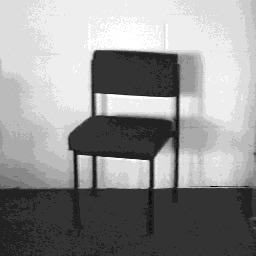
\includegraphics[width=0.22\textwidth]{img/orig/chair.jpg}}\quad
    \subfigure[Histograma]
    {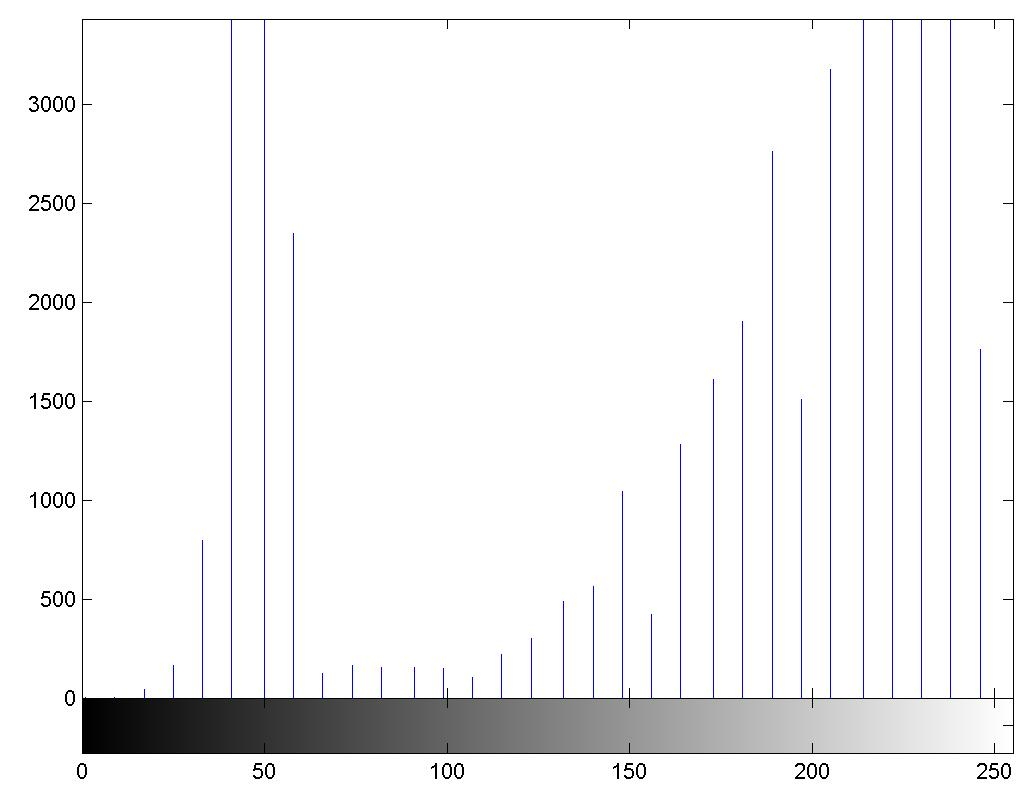
\includegraphics[width=0.28\textwidth]{img/hist/hist-chair.jpg}}\\
    \subfigure[`Bloques']    
    {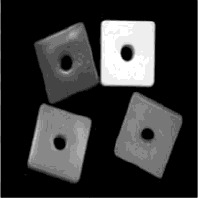
\includegraphics[width=0.22\textwidth]{img/orig/block.jpg}}\quad
    \subfigure[Umbralización del experto.]
    {
\includegraphics[width=0.22\textwidth]{img/orig/blockbin.jpg}}\quad
    \subfigure[Histrograma]
    {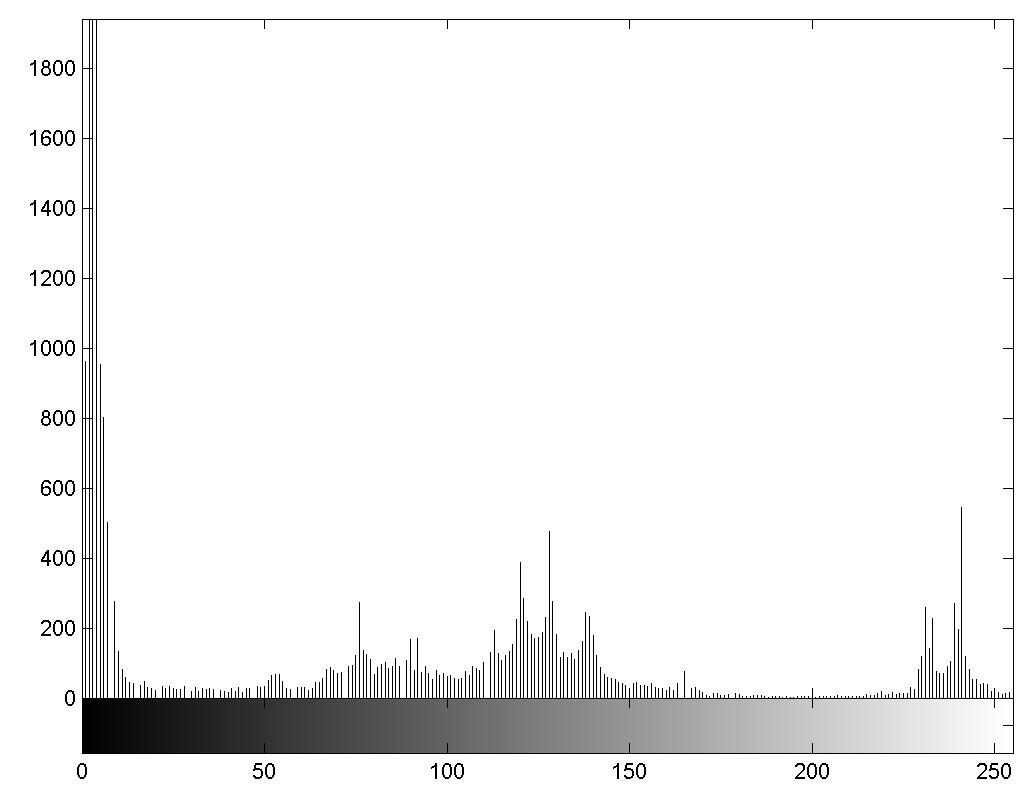
\includegraphics[width=0.28\textwidth]{img/hist/hist-block.jpg}}\\
    \subfigure[`Engranaje']
    {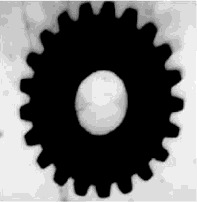
\includegraphics[width=0.22\textwidth]{img/orig/02.jpg}}\quad
    \subfigure[Umbralización del experto.]
    {
\includegraphics[width=0.22\textwidth]{img/orig/02bin.jpg}}\quad
    \subfigure[Histrograma]
    {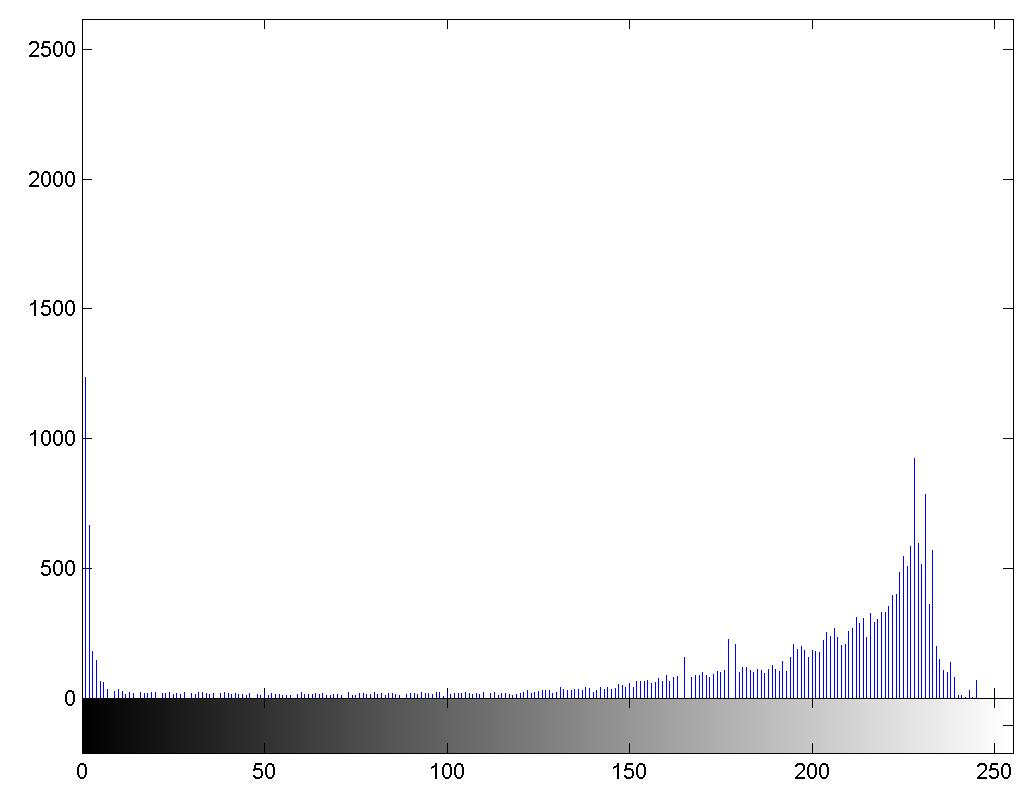
\includegraphics[width=0.28\textwidth]{img/hist/hist-02.jpg}}\\
    %\subfigure[`Piedras']
    %{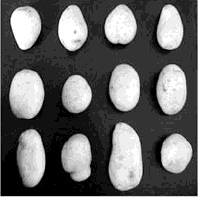
\includegraphics[width=0.22\textwidth]{img/orig/04.jpg}}\quad
    %\subfigure[Umbralización del experto.]
    %{
\includegraphics[width=0.22\textwidth]{img/orig/04bin.jpg}}\quad
    %\subfigure[Histrograma]
    %{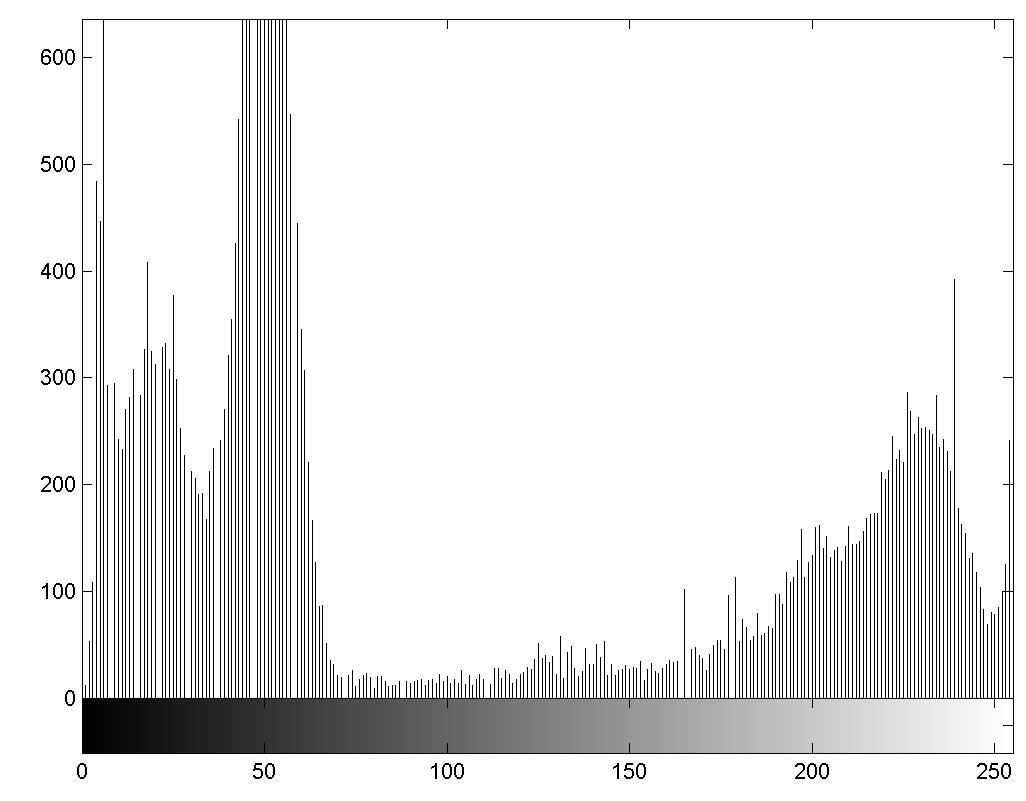
\includegraphics[width=0.28\textwidth]{img/hist/hist-04.jpg}}\\
    \subfigure[`Letras']
    {
\includegraphics[width=0.22\textwidth]{img/orig/09.jpg}}\quad
    \subfigure[Umbralización del experto.]
    {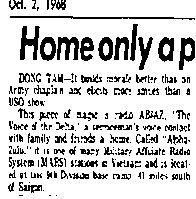
\includegraphics[width=0.22\textwidth]{img/orig/09bin.jpg}}\quad
    \subfigure[Histrograma]
    {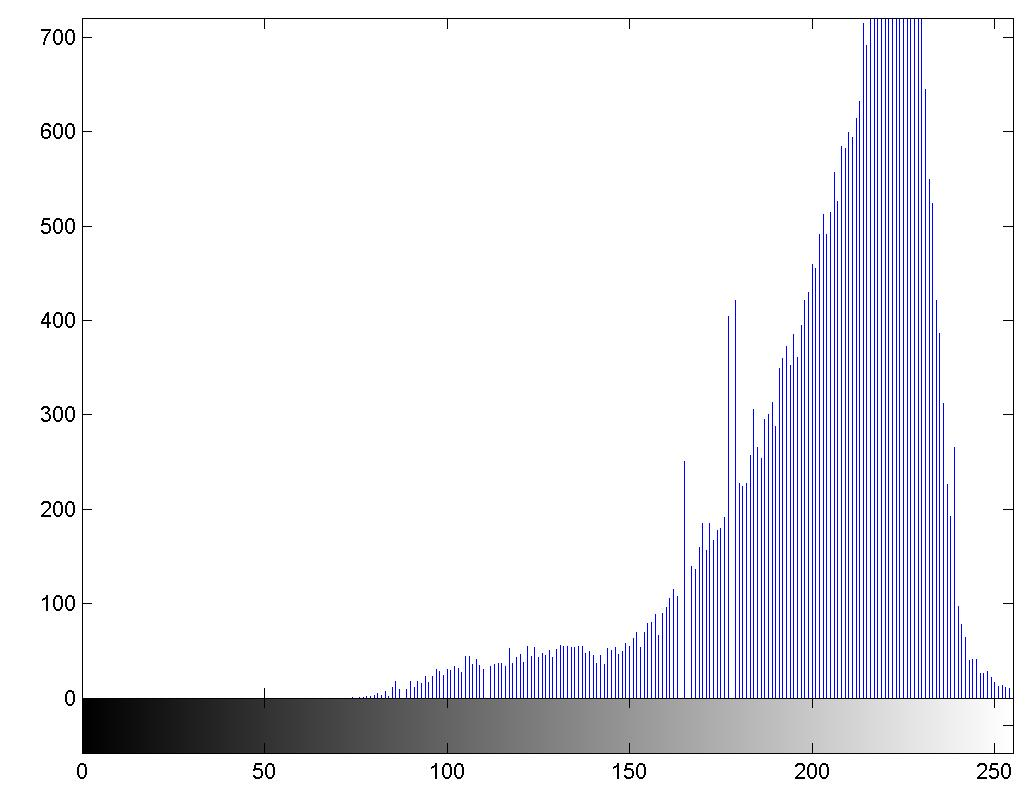
\includegraphics[width=0.28\textwidth]{img/hist/hist-09.jpg}}
    \subfigure[`Sombra']
    {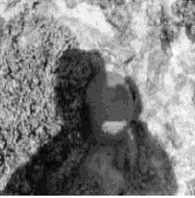
\includegraphics[width=0.22\textwidth]{img/orig/07.jpg}}\quad
    \subfigure[Umbralización del experto.]
    {
\includegraphics[width=0.22\textwidth]{img/orig/07bin.jpg}}\quad
    \subfigure[Histrograma]
    {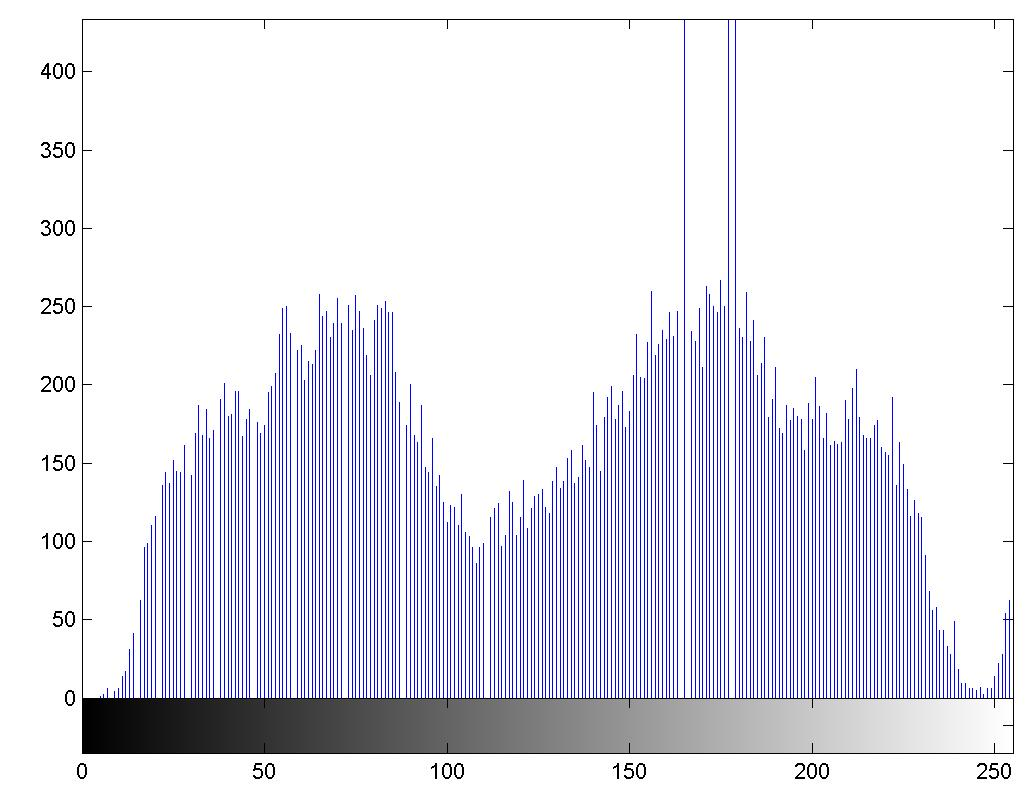
\includegraphics[width=0.28\textwidth]{img/hist/hist-07.jpg}}
    \caption{Imágenes utilizadas en el experimento 1 y siguientes.}
    \label{fig:imagenes}
\end{figure}

%\REV{faltan histogramas figura \ref{fig:sillaconruido}} Solucionado
%\REV{incluir figura con maximo contraste}
%\begin{figure}
%\centering
%    \subfigure[Muy alto contraste]
%    {\includegraphics[width=0.22\textwidth]{img/orig/chairmuyacon.jpg}}\quad
%    \subfigure[Alto contraste]
%    {\includegraphics[width=0.22\textwidth]{img/orig/chairacon.jpg}}\quad
%    \subfigure[Bajo contraste]
%    {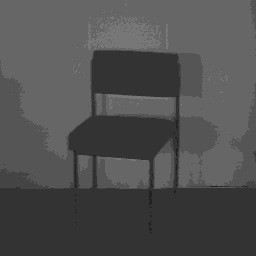
\includegraphics[width=0.22\textwidth]{img/orig/chairbcon.jpg}}\quad
%    \subfigure[Muy bajo contraste]    
%    {
\includegraphics[width=0.22\textwidth]{img/orig/chairmuybcon.jpg}}
%    \caption{Imágenes con ruido utilizadas en el experimento 1 y siguientes.}
%    \label{fig:sillaconcontraste}
%\end{figure}

\subsubsection{Resultados}
En la tabla \ref{tab:resultexp1dombi} se pueden apreciar los resultados para la umbralización de cada una de las imágenes y diferentes $w$. Se dispone, también de la tabla \ref{tab:resultexp1otros} donde se expresan los umbrales para otros algoritmos. En la comparación de ambas tablas se obtiene un resultado claro, el parámetro $w$ influye de forma determinante en la segmentación de las imágenes. Así, por ejemplo, en el caso de la `silla' $w=1$ es una opción totalmente acertada mientras que para para las `letras' habría que doblar el valor para obtener una umbralización igual de buena en comparación con los otros métodos.

\begin{table}
\centering
\begin{tabular}{c||c|c|c|c|c} 
$\mathbf{w}$    &\bb Silla&\bb Bloques&\bb Engranaje&\bb Letras&\bb Sombra\\\hline\hline
$\mathbf{0,1}$  &   218   &    255    &     250     &   142    &   200  \\\hline
$\mathbf{0,5}$  &   226   &    255    &     250     &    39    &   230  \\\hline
$\mathbf{0,75}$ &    95   &    119    &     115     &   103    &   111  \\\hline
$\mathbf{1}$    &   127   &    123    &     137     &   160    &   125  \\\hline
$\mathbf{1,25}$ &    70   &     97    &      96     &    80    &    91  \\\hline
$\mathbf{1,5}$  &    45   &     79    &      0      &    39    &    64  \\\hline
$\mathbf{2}$    &   144   &     76    &     138     &   197    &    96  \\\hline
$\mathbf{5}$    &   218   &     31    &      59     &   216    &   219  \\\hline
\end{tabular}
\caption{Umbrales para cada imagen con la función de Dombi y diferentes $w$.\label{tab:resultexp1dombi}}
\end{table}

\begin{table}
\centering
\begin{tabular}{c||c|c|c|c|c} 
                                                  &\bb Silla&\bb Bloques&\bb Engranaje&\bb Letras&\bb Sombra\\\hline\hline
\bb Alg. 1 con $\mathbf{REF_1=1-\abs{x-y}}$         &   127   &     79    &     104     &   187    &   123  \\\hline
\bb Alg. 1 con $\mathbf{REF_1=1-\abs{x-y}^2}$       &   127   &     97    &     140     &   179    &   126  \\\hline
\bb Alg. 1 con $\mathbf{REF_1=1-\abs{x-y}^{0.5}}$   &   119   &     47    &      84     &   200    &   121  \\\hline
\bb Alg. 1 con $\mathbf{REF_1=(1-\abs{x-y})^2}$     &   127   &     70    &     105     &   190    &   123  \\\hline
\bb Alg. 1 con $\mathbf{REF_1=(1-\abs{x-y})^{0.5}}$ &   127   &     82    &     104     &   186    &   124  \\\hline
\bb U. Global                                       &   130   &     79    &     105     &   187    &   124  \\\hline
\bb U. de Otsu                                      &   123   &     79    &     104     &   187    &   123  \\\hline
\bb Máx. la entropía de Renyi                       &   170   &     32    &     131     &   160    &   135  \\\hline
\end{tabular}
\caption{Umbrales para cada imagen con otras versiones de algoritmos.\label{tab:resultexp1otros}}
\end{table}

Por otra parte, cabe destacar que este resultado se ha obtenido en un tiempo de computación de alrededor de 0,0025 segundos, tanto para la versión con función de Dombi como para la de REF. Con la intención de que el lector pueda juzgar adecuadamente estos resutlados, se presentan los resultados, en forma gráfica, para aquellos valores de $w$ más reelevantes de forma gráfica en la tabla \ref{tab:resultexp1imagenesdombi}. Se facilita la posibilidad de poder compararlo directamente con el algoritmo original. Además, se dispone en el apéndice, en la tabla \ref{tab:otrassegmentaciones}, la umbralización de las imágenes con otros algoritmos para que se pueda llevar a cabo también la comparación.

\begin{table}
\centering
\begin{tabular}{c||c|c|c} 
$\mathbf{REF_1=1-\abs{x-y}}$ & $\mathbf{w=0,75}$ &\bb $\mathbf{w=1}$ &\bb $\mathbf{w=1,25}$\\\hline\hline
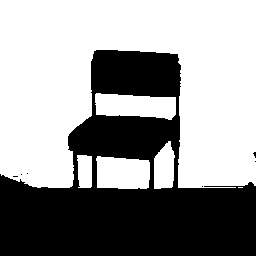
\includegraphics[width=0.2\textwidth]{img/res/e1a/alg1tipo1-chair.jpg} &
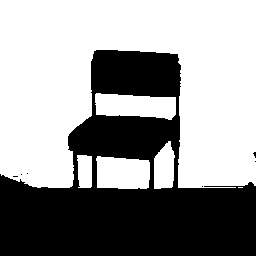
\includegraphics[width=0.2\textwidth]{img/res/e1a/alg1tipo6-chair.jpg} &
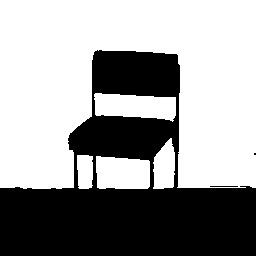
\includegraphics[width=0.2\textwidth]{img/res/e1a/alg1tipo6d0.75-chair.jpg} &
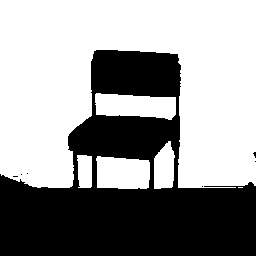
\includegraphics[width=0.2\textwidth]{img/res/e1a/alg1tipo6d1.25-chair.jpg} \\

\includegraphics[width=0.2\textwidth]{img/res/e1a/alg1tipo1-block.jpg} &

\includegraphics[width=0.2\textwidth]{img/res/e1a/alg1tipo6-block.jpg} &

\includegraphics[width=0.2\textwidth]{img/res/e1a/alg1tipo6d0.75-block.jpg} &

\includegraphics[width=0.2\textwidth]{img/res/e1a/alg1tipo6d1.25-block.jpg} \\

\includegraphics[width=0.2\textwidth]{img/res/e1a/alg1tipo1-02.jpg} &

\includegraphics[width=0.2\textwidth]{img/res/e1a/alg1tipo6-02.jpg} &

\includegraphics[width=0.2\textwidth]{img/res/e1a/alg1tipo6d0.75-02.jpg} &

\includegraphics[width=0.2\textwidth]{img/res/e1a/alg1tipo6d1.25-02.jpg} \\
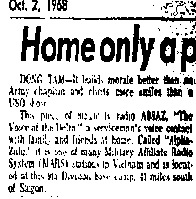
\includegraphics[width=0.2\textwidth]{img/res/e1a/alg1tipo1-09.jpg} &
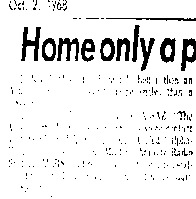
\includegraphics[width=0.2\textwidth]{img/res/e1a/alg1tipo6-09.jpg} &

\includegraphics[width=0.2\textwidth]{img/res/e1a/alg1tipo6d0.75-09.jpg} &
\includegraphics[width=0.2\textwidth]{img/res/e1a/alg1tipo6d1.25-09.jpg} \\
\includegraphics[width=0.2\textwidth]{img/res/e1a/alg1tipo1-07.jpg} &
\includegraphics[width=0.2\textwidth]{img/res/e1a/alg1tipo6-07.jpg} &
\includegraphics[width=0.2\textwidth]{img/res/e1a/alg1tipo6d0.75-07.jpg} &
\includegraphics[width=0.2\textwidth]{img/res/e1a/alg1tipo6d1.25-07.jpg} \\\hline
\end{tabular}
\caption{Resultado de las segmentaciones para el algoritmo con REF y Dombi con varios $w = \{0,75; 1; 1,25\}$.\label{tab:resultexp1imagenesdombi}}
\end{table}

Para poder comprobar y comparar formalmente todos los resultados, se calcula el error cuadrático medio para las imágenes. En concreto, se hace con todas las versiones obtenidas con otros los algoritmos presentados sin obtener ningún resultado reelevante. Se presentan en la tabla \ref{tab:erroresexp1dombi}, la comparación que se hace entre las segmentaciones que se obtienen con varias $w$ y la imagen umbralizada de forma exacta por un experto, resultados que se hacen más interesantes que los anteriores. De nuevo, de esta tabla se desprende de que en función de la imagen que se tome, el parámetro $w$ para obtener una mejor umbralización.

\begin{table}
\centering
\begin{tabular}{c||c|c|c|c} 
$\mathbf{w}$                    &\bb Bloques&\bb Engranaje&\bb Letras&\bb Sombra\\\hline\hline
\bb Alg. 1 con $\mathbf{0,75}$  &   43,3750  &   33,0080   &   33,3617   &   59,2420  \\\hline
\bb Alg. 1 con $\mathbf{1}$     &   49,8760  &   36,3914   &   29,6418   &   52,0672  \\\hline
\bb Alg. 1 con $\mathbf{1,25}$  &   50,0241  &   32,0153   &   31,0001   &   55,0322  \\\hline
\end{tabular}
\caption{Errores para las imágenes con ruido con otras versiones de algoritmos.\label{tab:erroresexp1dombi}}
\end{table}


%Con ruido
Con la intención de poder llevar a cabo experimentos sobre imágenes con ruido, se crean estas de forma sintética, tal y como se ha presentando en la sección \ref{sec:ruido}. Se pueden ver los resultados sobre la imagen `silla', y sus histogramas, en la figura \ref{fig:imagenesruido}. 

\begin{figure}
\centering
    \subfigure[Ruido gausiano]
    {\includegraphics[width=0.25\textwidth]{img/orig/chairga.jpg}}\quad
    \subfigure[Ruido `sal y pimienta' con $p=0,05$]
    {\includegraphics[width=0.25\textwidth]{img/orig/chairs&p005.jpg}}\quad
    \subfigure[Ruido `sal y pimienta' con $p=0,2$]    
    {\includegraphics[width=0.25\textwidth]{img/orig/chairs&p020.jpg}}
    \subfigure[Histograma de ruido gausiano]
    {\includegraphics[width=0.3\textwidth]{img/hist/hist-chairga.jpg}}\quad
    \subfigure[Histograma de ruido `sal y pimienta' con $p=0,05$]
    {\includegraphics[width=0.3\textwidth]{img/hist/hist-chairsp005.jpg}}\quad
    \subfigure[Histograma de ruido `sal y pimienta' con $p=0,2$]    
    {\includegraphics[width=0.3\textwidth]{img/hist/hist-chairsp020.jpg}}
    \caption{Imágenes con ruido utilizadas en el experimento 1 y siguientes.}
    \label{fig:imagenesruido}
\end{figure}

Los umbrales que se han obtenido se expresan en la tabla \ref{tab:resultexp1ruido}. Comparándola de nuevo con otros algoritmos (tablas \ref{tab:resultexp1ruidootros}), se puede apreciar que se pueden obtener resultados similiares también e, igualmente, que el parámetro $w$ es decisivo para diferentes imágenes. Es curioso comprobar el hecho de que con la misma $w$ se obtienen resultados similares en comparación con los umbrales de la versión original con REF. 

\begin{table}
\centering
\begin{tabular}{c||c|c|c} 
           &\bb R. gausiano&\bb R. impulsivo 0.05&\bb R. impulsivo 0.2\\\hline\hline
$\mathbf{0,1}$  &   219   &    226    &     226     \\\hline
$\mathbf{0,5}$  &   234   &    226    &     242     \\\hline
$\mathbf{0,75}$ &    99   &     95    &      95     \\\hline
$\mathbf{1}$    &   128   &    127    &     127     \\\hline
$\mathbf{1,25}$ &    74   &     70    &      62     \\\hline
$\mathbf{1,5}$  &    35   &     45    &      37     \\\hline
$\mathbf{2}$    &   147   &    136    &     127     \\\hline
$\mathbf{5}$    &   226   &    218    &     226     \\\hline
\end{tabular}
\caption{Umbrales para las imágenes con ruido con la función de Dombi y diferentes valores de $w$.\label{tab:resultexp1ruido}}
\end{table}


\begin{table}
\centering
\begin{tabular}{c||c|c|c} 
                          &\bb R. gausiano&\bb R. impulsivo 0.05&\bb R. impulsivo 0.2\\\hline\hline
\bb Alg. 1 con $\mathbf{REF_1=1-\abs{x-y}}$             &   132   &    127    &     127     \\\hline
\bb Alg. 1 con $\mathbf{REF_1=1-\abs{x-y}^2}$           &   131   &    127    &     127     \\\hline
\bb Alg. 1 con $\mathbf{REF_1=1-\abs{x-y}^{0.5}}$       &   131   &    136    &     152     \\\hline
\bb Alg. 1 con $\mathbf{REF_1=(1-\abs{x-y})^2}$         &   132   &    127    &     127     \\\hline
\bb Alg. 1 con $\mathbf{REF_1=(1-\abs{x-y})^{0.5}}$     &   131   &    127    &     127     \\\hline
\bb U. Global                                           &   132   &    130    &     128     \\\hline
\bb U. de Otsu                                          &   132   &    123    &     123     \\\hline
\bb Máx. la entropía de Renyi                           &   154   &    170    &     170     \\\hline
\end{tabular}
\caption{Umbrales para las imágenes con ruido con otras versiones de algoritmos.\label{tab:resultexp1ruidootros}}
\end{table}

En cuanto al tiempo de cómputo, de nuevo vuelven a estar todos los valores entorno a 0,0025 segundos. Esto hace ver que el método presentado sigue siendo igual de eficiente que la versión original. Así mismo, se muestran los resultados gráficamente en la tabla \ref{tab:resultexp1imagenesruido}.

\begin{table}
\centering
\begin{tabular}{c||c|c|c} 
$\mathbf{REF_1=1-\abs{x-y}}$ & $\mathbf{w=0,75}$ &\bb $\mathbf{w=1}$ &\bb $\mathbf{w=1,25}$\\\hline\hline
\includegraphics[width=0.2\textwidth]{img/res/e1a/alg1tipo1-chairga.jpg} &
\includegraphics[width=0.2\textwidth]{img/res/e1a/alg1tipo6-chairga.jpg} &
\includegraphics[width=0.2\textwidth]{img/res/e1a/alg1tipo6d0.75-chairga.jpg} &
\includegraphics[width=0.2\textwidth]{img/res/e1a/alg1tipo6d1.25-chairga.jpg} \\
\includegraphics[width=0.2\textwidth]{img/res/e1a/alg1tipo1-chairsp005.jpg} &
\includegraphics[width=0.2\textwidth]{img/res/e1a/alg1tipo6-chairsp005.jpg} &
\includegraphics[width=0.2\textwidth]{img/res/e1a/alg1tipo6d0.75-chairsp005.jpg} &
\includegraphics[width=0.2\textwidth]{img/res/e1a/alg1tipo6d1.25-chairsp005.jpg} \\
\includegraphics[width=0.2\textwidth]{img/res/e1a/alg1tipo1-chairsp020.jpg} &
\includegraphics[width=0.2\textwidth]{img/res/e1a/alg1tipo6-chairsp020.jpg} &
\includegraphics[width=0.2\textwidth]{img/res/e1a/alg1tipo6d0.75-chairsp020.jpg} &
\includegraphics[width=0.2\textwidth]{img/res/e1a/alg1tipo6d1.25-chairsp020.jpg} \\\hline
\end{tabular}
\caption{Umbrales para las imágenes con ruido con otras versiones de algoritmos.\label{tab:resultexp1imagenesruido}}
\end{table}

En relación con los errores con imagenes umbralizadas con otros algoritmos, no se obtiene ningún resultado concluyente ya que en ningún momento el error pasa de 0,1.

Además, se han hecho experimentos con imágenes con mucho y poco contraste. En este caso, la solución tenía el error de nuevo en un rango de diferencia de una décima, aunque permite llegar a opciones con mucho más bajo contraste que el algoritmo de la maximización de la entropía de Renyi, que es el que mejor lo hace entre los otros algoritmos presentados. En definitiva, con el algoritmo de maximización de la similitud se pueden llegar a segmentar imágenes con intervalos de menos de 15 niveles de gris. Se encuentra, también, el hechod de que en el caso de crear dos imágenes con alto y bajo contraste que sean ``contrarias'', la segmentación que se obtiene es la misma.


% EXPERIMENTO 2
\subsection{Experimento 2: busqueda del mejor umbral a través de funciones penalti\label{sec:exp2}}
\subsubsection{Explicación del experimento}
En vista del experimento anteior donde había momentos en los que la función de dombi no actuaba de forma correcta, se propone una nueva forma para poder elegir entre la función de Dombi o volver al método con la función REF. En concreto, se intentará dilucidar esta situación por medio de una función penalti. El proceso de la obtención del conjunto difuso cambiará, ya que no será una única función y tendrá el siguiente orden:
\begin{enumerate}
    \item Creación de todas las pertenencias con las 5 funciones REF presentadas y la función de Dombi con $w=1$.
    \item Agregación de todas las pertenencias anteriores con varias funciones, a saber:
        \begin{enumerate}
            \item Media aritmética.
            \item Media geométrica.
            \item Máximo.
            \item Mínimo.
            \item Integral Choquet.
            \item OWA de `al menos la mitad'. %\REV{nombre}
        \end{enumerate}    
    \item Con todos estos resultados se actua con la función penalti para cada uno de los elementos $a_1,\dots a_n$ agregados y las pertenencias obtenidas en (1) $r=(r_1,\dots, r_m)$, obtendremos $p(a_i, r)=\sum_{j=1}^m \abs{a_i-r_j}$.
    \item Cogeremos como pertenencia aquel resultado de la agregación, $a_i$, que haga que el resultado de la función penalti sea máximo.  
\end{enumerate}

En vista de que los resultados de la idea presentada anteriormente no presentaba a penas diferencia con el experimento 1. Por esta razón, en una segunda versión, se añadirá también la función de agregación siguiente con la intención de crear más {\em outlayers} que creen más posibles umbrales.
$$M_{zadeh}(r_1,\dots,r_m)=\max\left(0, \sum r-(n-1)\right)\cdot \sqrt[n]{\prod_{i=1}^n{r_i}}$$
Esta segunda versión son los resultados que se presentan a continuación.

\subsubsection{Resultados}

En la tabla \ref{tab:resultexp2agregado} se recogen los umbrales $t$ creados a través de la función penalti. De nuevo, en comparación con los presentados en la tabla \ref{tab:resultexp1otros} se puede observar que siempre son valores que se encuentran en el intervalo que pueden definir. Esto hace suponer que las imágenes tiene una umbralización correcta, algo que se puede comprobar con las imágenes del cuadro \ref{tab:resultexp2imagenagregado}. En relación al error (tabla \ref{tab:resultexp2agregado})sorprende la diferencia que existe frente

\begin{table}
\centering
\begin{tabular}{c|c|c|c|c} 
\bb Silla&\bb Bloques&\bb Engranaje&\bb Letras&\bb Sombra\\\hline\hline
   127   &     68    &      92     &   196    &   123  \\\hline
\end{tabular}
\caption{Umbrales para cada imagen con el algoritmo 1 calculando la función de pertenencia a través de una función penalti.\label{tab:resultexp2agregado}}
\end{table}


\begin{table}
\centering
\begin{tabular}{ccccc}\hline
\includegraphics[width=0.15\textwidth]{img/res/e2a/alg1agregate-chair.jpg} &
\includegraphics[width=0.15\textwidth]{img/res/e2a/alg1agregate-block.jpg} &
\includegraphics[width=0.15\textwidth]{img/res/e2a/alg1agregate-02.jpg} &
\includegraphics[width=0.15\textwidth]{img/res/e2a/alg1agregate-09.jpg} &
\includegraphics[width=0.15\textwidth]{img/res/e2a/alg1agregate-07.jpg}\\\hline
\end{tabular}
\caption{Resultado para el nuevo algoritmo a través de penalti con todas las funciones propuestas.\label{tab:resultexp2imagenagregado}}
\end{table}


\begin{table}
\centering
\begin{tabular}{c|c|c|c|c} 
\bb Bloques&\bb Engranaje&\bb Letras&\bb Sombra\\\hline\hline
     90,3727    &      124,9112     &     140,5241    &     194,3489  \\\hline
\end{tabular}
\caption{Errores en comparación con las imágenes segmentadas por el experto.\label{tab:erroresexp2agregado}}
\end{table}


Además, en la tabla \ref{tab:resultexp2agregadoruido} se pueden observar los umbrales obtenidos para las imágenes con ruido. De forma similar a las imágenes normales, el umbral vuelve a estar en el intervalo que se crea con los umbrales originales del experimento anterior. Tal y como se puede ver en la tabla \ref{tab:resultexp2imagenagregadoruido} el resultado para las imágenes con ruido gausiano y con ruido `sal y pimienta' con $p=0,05$ mientras que subiendo la probabilidad para el ruido, el umbral comienza a ser bastante inadecuado. Como es lógico, el ruido impulsivo no se consigue resolver aunque tampoco es así en el caso del gausiano, que segmenta de forma bastante adecuada aun no apreciandose un mínimo claro.

\begin{table}
\centering
\begin{tabular}{c|c|c} 
\bb R. gausiano&\bb R. impulsivo 0.05&\bb R. impulsivo 0.2\\\hline\hline
   132   &     127    &      152    \\\hline
\end{tabular}
\caption{Umbrales para cada imagen ruido a través del algoritmo 1 calculando la función de pertenencia a través de una función penalti.\label{tab:resultexp2agregadoruido}}
\end{table}


\begin{table}
\centering
\begin{tabular}{ccc}\hline
\includegraphics[width=0.2\textwidth]{img/res/e2a/alg1agregate-chairga.jpg} &
\includegraphics[width=0.2\textwidth]{img/res/e2a/alg1agregate-chairsp005.jpg} &
\includegraphics[width=0.2\textwidth]{img/res/e2a/alg1agregate-chairsp020.jpg}\\\hline
\end{tabular}
\caption{Resultado para el nuevo algoritmo a través de penalti con todas las funciones propuestas para imágenes con ruido.\label{tab:resultexp2imagenagregadoruido}}
\end{table}



% EXPERIMENTO 3
\subsection{Experimento 3: sustitución de la función REF por la función de Dombi en el algoritmo para la obtenición del umbral óptimo}

\subsubsection{Explicación del experimento}
En este experimento se ha tomado el algoritmo de obtención del umbal óptimo maximizando la similitud (algoritmo 3A) para comprobar el efecto de la función de Dombi en él. Por esta razón, y en vista de los resultados del experimento 1, se plantean dos variantes. En primer lugar, se incorpora la función de dombi a las 5 funciones REF que ya estaban para poder ver qué umbral se obtiene, intentando escoger el mejor (algoritmo 3B). Después, se eligen los diferentes valores de $w$ que se han utilizado antes (algoritmo 3C). De esta forma, se intenta buscar cual de los umbrales calculados anteriormente de forma individual es el mejor.

\subsubsection{Resultados}

Hecho todo el cómputo, en la tabla \ref{tab:resultexp3dombi} se muestran los umbrales obtenidos tanto con el algoritmo original como por parte de las dos versiones que se han propuesto. Por un lado, es muy visible el hecho de que para la mayor parte de las imágenes la versión C no tiene utilidad, ya que elige umbrales totalmente fuera de la lógica. Por otra parte, se ve que la versión B es muy similar a la versión original. Esto hace pensar que esta versión podría hacer que las funciones de Dombi fueran interesantes para algunos casos. Los resultados gráficos se presentan en la tabla \ref{tab:resultexp3imagenesdombi}

\begin{table}
\centering
%\resizebox*{3\textwidth}{!}{
\begin{tabular}{c||c|c|c|c|c} 
             &\bb Silla&\bb Bloques&\bb Engranaje&\bb Letras&\bb Sombra\\\hline\hline
\bb Alg. 3A  &   115   &    80    &     88      &    199   &    121   \\\hline
\bb Alg. 3B  &   127   &    123    &     84      &    200   &    125   \\\hline
\bb Alg. 3C  &   218   &    254    &     250     &    142   &    219   \\\hline
\end{tabular}
\caption{Umbrales para cada imagen con el algoritmo 3 en todas sus nuevas versiones.\label{tab:resultexp3dombi}}
\end{table}


\begin{table}
\centering
\begin{tabular}{cccccc}\hline
Alg. 3B\quad
\includegraphics[width=0.15\textwidth]{img/res/e3a/alg3btipo-chair.jpg} &
\includegraphics[width=0.15\textwidth]{img/res/e3a/alg3btipo-block.jpg} &
\includegraphics[width=0.15\textwidth]{img/res/e3a/alg3btipo-02.jpg} &
\includegraphics[width=0.15\textwidth]{img/res/e3a/alg3btipo-09.jpg} &
\includegraphics[width=0.15\textwidth]{img/res/e3a/alg3btipo-07.jpg}\\\hline
Alg. 3C\quad     
\includegraphics[width=0.15\textwidth]{img/res/e3a/alg3ctipo-chair.jpg} &
\includegraphics[width=0.15\textwidth]{img/res/e3a/alg3ctipo-block.jpg} &
\includegraphics[width=0.15\textwidth]{img/res/e3a/alg3btipo-02.jpg} &
\includegraphics[width=0.15\textwidth]{img/res/e3a/alg3ctipo-09.jpg} &
\includegraphics[width=0.15\textwidth]{img/res/e3a/alg3ctipo-07.jpg}\\\hline
\end{tabular}
\caption{Resultado gráfico con el algoritmo 3 con las nuevas propuestas.\label{tab:resultexp3imagenesdombi}}
\end{table}

En cuanto al tiempo de cómputo, aunque crece con respecto a los algoritmos de los experimentos anteriores, este sigue estando en la misma media del algoritmo original, siempre que se tome como versión original la que definen las 5 REF del algoritmo 1. Todos los resultados gráficos son resumidos en la tabla \ref{tab:resultexp3imagenesdombi}.

%\REV{errores, imposible que sean esos...}

Para poder conocer cómo de buenos son los resultados, se comparan las imágenes obteniendo el error cuadrático medio (tabla\ref{tab:erroresexp3otros}). En esta se puede apreciar cómo se mantiene un error bastante similar con todos los algoritmos.

%\begin{table}
%\centering
%\begin{tabular}{c||c|c|c|c}
%                &\bb Bloques  &\bb Engranaje&\bb Letras  &\bb Sombra  \\\hline\hline
%\bb Alg. 3B     &   0,0082   &   124,9112   &   0,2019   &   0,1017   \\\hline
%\bb Alg. 3C     &     0      &   124,9112   &   0,0136   &   0,5744   \\\hline
%\end{tabular}
%\caption{Errores de las imágenes perfectas para cada imagen con el algoritmo 3 en todas sus versiones.\label{tab:erroresexp3dombi}}
%\end{table}


\begin{table}
\centering
\begin{tabular}{c||c|c|c|c}
                        &\bb Silla    &\bb Bloques  &\bb Engranaje &\bb Sombra    \\\hline\hline
\bb Alg. 3A (Original)  &   72,8822   &   93,8135   &   126,5836   &   124,7987   \\\hline
\bb Umb. Global         &   71,7070   &   81,0453   &   124,7637   &   122,4343   \\\hline
\bb {\em K-means}       &   71,7070   &   81,0453   &   124,9112   &   123,2863   \\\hline
\bb Método de Otsu      &   71,7070   &   81,0453   &   124,9112   &   123,2863   \\\hline
\bb Máx. Entropía Renyi &   56,9290   &   96,4543   &   121,5597   &   112,4747   \\\hline
\end{tabular}
\caption{Erorres de las imágenes obtenidas con otros algoritmos para cada imagen con el algoritmo 3 en todas sus versiones.\label{tab:erroresexp3otros}}
\end{table}


Se comprueba que las tendencias anteriores son también seguidas por aquellas imágenes que disponen de ruido. Es decir, la versión que se propone con la función de dombi con diferentes valores de $w$. También, los resultados con la versión B son más bajos con respecto a las versión original, algo que como se ha visto es bastante común desde el momento en el que se introducen las funciones de Dombi.


\begin{table}
\centering
\begin{tabular}{c||c|c|c}
        &\bb R. gausiano&\bb R. impulsivo 0.05&\bb R. impulsivo 0.2\\\hline\hline
\bb Alg. 3A  &   131   &    136    &     144      \\\hline
\bb Alg. 3B  &   128   &    127    &     127      \\\hline
\bb Alg. 3C  &   226   &    218    &     226      \\\hline
\end{tabular}
\caption{Umbrales para cada imagen ruidosa con el algoritmo 3 en todas sus versiones.\label{tab:resultexp3ruido}}
\end{table}



\begin{table}
\centering
\begin{tabular}{cccccc}\hline
Alg. 3B\quad
\includegraphics[width=0.18\textwidth]{img/res/e3a/alg3btipo-chairga.jpg} &
\includegraphics[width=0.18\textwidth]{img/res/e3a/alg3btipo-chairsp005.jpg} &
\includegraphics[width=0.18\textwidth]{img/res/e3a/alg3btipo-chairsp020.jpg}\\\hline
Alg. 3C\quad     
\includegraphics[width=0.18\textwidth]{img/res/e3a/alg3ctipo-chairga.jpg} &
\includegraphics[width=0.18\textwidth]{img/res/e3a/alg3ctipo-chairsp005.jpg} &
\includegraphics[width=0.18\textwidth]{img/res/e3a/alg3ctipo-chairsp020.jpg}\\\hline
\end{tabular}
\caption{Representación gráfica del resultado .\label{tab:resultexp3imagenesruido}}
\end{table}


\begin{table}
\centering
\begin{tabular}{c||c|c|c}
        &\bb R. gausiano&\bb R. impulsivo 0.05&\bb R. impulsivo 0.2\\\hline\hline
\bb Alg. 3 Original     &   95,1075   &   66,4737   &   74,2907   \\\hline
\bb Umb. Global         &   94,8740   &   68,2635   &   77,5124   \\\hline
\bb {\em K-means}       &   95,1074   &   68,2635   &   77,5124   \\\hline
\bb Método de Otsu      &   94,8740   &   68,2635   &   77,5124   \\\hline
\bb Máx. Entropía Renyi &   85,9364   &   54,1976   &   65,7772   \\\hline
\end{tabular}
\caption{Errores para cada imagen ruidosa con otros algoritmos tomando como referencia la versión 3B.\label{tab:erroresexp3ruido}}
\end{table}



\subsection{Repetición de los experimentos con la corrección oportuna.}\label{sec:cambiodombi}
Vistos los resultados de los experimentos anteriores, y en especial el que se refiere al experimento 3, se plantea el porqué se obtiene un resultado tan malo. Este hecho es extraño sobre todo por el hecho de que a través de los diferentes valores de $w$, el algoritmo 1 con las funciones de dombi siempre tiene buenos resultados. Se comprueba el vector de similitudes que se obtiene para dilucidar qué umbral escoger en el algoritmo 3, lo que muestra que la similitud mayor no se encuentra en el mejor umbral. %\REV{¿ejemplo?}

Reestudiando la situación, se encuentra que en las propiedades de las funciones que propone Dombi (Lema \ref{def:propiedadesdombi}) se ha omitido que una función de equivalencia $e$ cumple $e(x,x)=1$. En particular, las funciones REF son un ejemplo de esta situación. La razón por la que no se puede cumplir esta propiedad es porque existe otra que dice $e(x,n(x))=0$. Como es evidente, el intentar mantener ambas a la vez es una contradicción. Por esta razón, el autor dice que sus funciones cumplirán en parte ambas en función de un parámetro. Esto hace que para dos elementos iguales no tengamos como resultado 1. 

Vista la situación y sabiendo que la construcción que se utiliza para los conjuntos difusos hace necesario que la condición anterior se cumpla de forma plena, se intenta reescribir la función de pertenencia a los conjuntos difusos. De esta forma, se aplica a todos los experimentos que se han mostrado anteriormente esta nueva función (ecuación \ref{eq:intentodesolucionardombi})

\begin{equation}\label{eq:intentodesolucionardombi}
    \mu_{Q_t}(q)=\left\{ \begin{split}
                 \min\left( 1, \frac
                    {\unmedio \left(1+\left(1-\frac{2q}{L-1}\right)\left(1-\frac{2m_b}{L-1}\right)\right)}
                    {\unmedio \left(1+\left(1-\frac{2m_b}{L-1}\right)\left(1-\frac{2m_b}{L-1}\right)\right)}\right)
                 \text{\quad si\quad} q\leq t\\
                 \min\left( 1, \frac
                    {\unmedio \left(1+\left(1-\frac{2q}{L-1}\right)\left(1-\frac{2m_o}{L-1}\right)\right)}
                    {\unmedio \left(1+\left(1-\frac{2m_o}{L-1}\right)\left(1-\frac{2m_o}{L-1}\right)\right)}\right)
                \text{\quad si\quad} q > t
                \end{split}\right.
\end{equation}



%RESULTADOS DE LA REESCRITURA
\subsubsection{Resultados}
La opción que se ha propuesto anteriormente ha tenido resultados muy malos, de hecho, mucho peores que las presentadas en las secciones anteirores. Por esa razón y únicamente a modo de ejemplo, en las tablas \ref{tab:resultexp1bdombi} y \ref{tab:resultexp3bdombi} se pueden ver algunos resultados obtenidos. Este algoritmo, es por tanto, desechado de forma completa. Se acaba concluyendo que las funciones de Dombi no pueden sustituir directamente a funciones REF tal y como el autor sugería. Por esta razón, la umbralización con los métodos anteriores presentará resultados hetereogéneos lo que hace que no sea un método útil para su utilización habitual.

\begin{table}\begin{center}
%\resizebox*{3\textwidth}{!}{
\begin{tabular}{cc||c|c|c|c|c} 
                                    &                   &\bb Silla&\bb Bloques&\bb Engranaje&\bb Letras&\bb Sombra\\\hline\hline
\bb{\multirow{2}{1.75cm}{$w=0,1$}}  &  \bb Umbral ($t$) &   234   &     8     &      0      &   157    &   250  \\
                                    &  \bb Tiempo (s)   &  0,002  &   0,675   &    0,686    &  0,689   &  0,688 \\\hline
\bb\multirow{2}{1.75cm}{$w=0,5$}    &  \bb Umbral ($t$) &   226   &     8     &     111     &   207    &   254  \\
                                    &  \bb Tiempo (s)   &  0,002  &   0,649   &    1,093    &  1,233   &  1,13  \\\hline
\bb\multirow{2}{1.75cm}{$w=0,75$}   &  \bb Umbral ($t$) &   226   &     8     &     122     &   182    &   238  \\
                                    &  \bb Tiempo (s)   &  0,002  &   0,677   &    0,686    &  0,688   &  0,679 \\\hline
\bb\multirow{2}{1.75cm}{$w=1$}      &  \bb Umbral ($t$) &   226   &     8     &      90     &   191    &   246  \\
                                    &  \bb Tiempo (s)   &  0,002  &   0,63    &    0,642    &  0,646   &  0,642 \\\hline
\bb\multirow{2}{1.75cm}{$w=1,25$}   &  \bb Umbral ($t$) &   226   &     8     &     250     &   203    &   252  \\
                                    &  \bb Tiempo (s)   &  0,002  &   0,682   &    0,684    &  0,688   &  0,686 \\\hline
\bb\multirow{2}{1.75cm}{$w=1,5$}    &  \bb Umbral ($t$) &   242   &     6     &     250     &   213    &   254  \\
                                    &  \bb Tiempo (s)   &  0,002  &   0,666   &    1,106    &  1,246   &  1,138 \\\hline
\bb\multirow{2}{1.75cm}{$w=2$}      &  \bb Umbral ($t$) &   250   &     3     &     250     &   215    &    66  \\
                                    &  \bb Tiempo (s)   &  0,002  &   0,631   &    0,640    &  0,644   &  0,641 \\\hline
\bb\multirow{2}{1.75cm}{$w=5$}      &  \bb Umbral ($t$) &   250   &     1     &     250     &   254    &    66  \\
                                    &  \bb Tiempo (s)   &  0,002  &   0,657   &    0,671    &  0,672   &  0,673 \\\hline
\end{tabular}\end{center}
\caption{Umbrales y tiempo de cómputo para cada imagen con el algoritmo 1 reescrito a través de funciones de Dombi.\label{tab:resultexp1bdombi}}
\end{table}

\begin{table}\begin{center}
\begin{tabular}{c||c|c|c} 
    &\bb Ruido gausiano&\bb Ruido impulsivo 0.05&\bb Ruido impulsivo 0.2\\\hline\hline
\bb Alg. 3A &   131   &    136    &     144     \\\hline
\bb Alg. 3B &   131   &    234    &     152     \\\hline
\bb Alg. 3C &   254   &    234    &     250    \\\hline
\end{tabular}\end{center}
\caption{Umbrales para versión del algoritmo 3 reescrito con imágenes ruidosas.\label{tab:resultexp3bdombi}}
\end{table}
\chapter{Segmentación de imágenes con agregando con funciones OWA}

En este capítulo se llevarán a cabo otro tipo de pruebas sobre los algoritmos presentados. Para ello, en primer lugar, se explicará el modo en el que se modificarán los algoritmos presentados en la sección \ref{sec:algoritmosmono}. Después se presentarán los resultados obtenidos con estas fórmulas, haciendo hincapié en los más interesantes.

%\section{Métodos algorítmicos de segmentación de un único umbral}
%\REV{Añadir todos aquellos detalles teóricos necesarios a tener en cuenta para continuar con los experimentos.}
%\input{contenidos/4-1-algoritmos}

\section{Experimentos y resultados con funciones de agregación OWA}

% EXPERIMENTO 4
\subsection{Experimento 4: sustitución de la media aritmética por funciones OWA en la construcción de los conjuntos difusos}
Para todos los experimentos que se disponen en este capítulo, tomaremos la determinación de sustituir la media aritmética que se utiliza en la construcción de los conjuntos difusos (def. \ref{def:mediasmonoumbral} y \ref{def:conjuntodifusomonoumbral}) por una función OWA de tipo `la mayoría de' (def. \ref{def:owa}). Para ello es importante destacar el hecho de que habrá que introducir todos los datos en forma normalizada (con valores en $[0,1]$).

En concreto, se utilizarán dos posibilidades de funciones OWA. La primera de ellas, OWA (1), crea los pesos según la ecuación \ref{eq:pesosowamayoria} habiendo ordenado el vector en función del histograma. En el segundo caso, OWA (2), crearemos los pesos de igual manera, pero en el momento de aplicarlos los multiplicaremos por la función $h(q)$ que les corresponda.

\subsubsection{Explicación del experimento}
En este primer experimento se sustituirá la media aritmética en la creación de los conjuntos difusos en el algoritmo 1. Se hará con las dos opciones de OWA presentadas. Se conoce de antemano, que debido a la necesidad del cálculo de los pesos, el tiempo de computación crecerá bastante frente a la versión original.


\subsubsection{Resultados}

En las tablas \ref{tab:resultexp4dombi} y \ref{tab:resultexp4ruido} se muestran los resultados obtenidos para todas las imágenes que se toman como muestra. Se ha de destacar que este experimento, al igual que todos, se ha llevado a cabo con un conjunto de casi 30 imágenes de las que se presentan las más significativas. 

Se puede observar que claramente los resultados obtenidos son extremadamente alejados de la realidad. Se crean únicamente umbrales que no permiten llevar a cabo ninguna segmentación de forma adecuada por lo que se omite la presentación de los resultados gráficos así como de los errores en este experimento.


\begin{table}
\centering
\begin{tabular}{c||c|c|c} 
\multicolumn{4}{c}{}\\
Silla                                &\bb Media&\bb OWA (1)&\bb OWA (2)\\\hline\hline
\bb Alg. 1 con $\mathbf{REF_1=1-\abs{x-y}}$         &   127 &   50  &   50  \\\hline
\bb Alg. 1 con $\mathbf{REF_1=1-\abs{x-y}^2}$       &   127 &   50  &   246 \\\hline
\bb Alg. 1 con $\mathbf{REF_1=1-\abs{x-y}^{0.5}}$   &   119 &   50  &   50  \\\hline
\bb Alg. 1 con $\mathbf{REF_1=(1-\abs{x-y})^2}$     &   127 &   50  &   50  \\\hline
\bb Alg. 1 con $\mathbf{REF_1=(1-\abs{x-y})^{0.5}}$ &   127 &   50  &   50  \\\hline
\multicolumn{4}{c}{}\\
Bloques                              &\bb Media&\bb OWA (1)&\bb OWA (2)\\\hline\hline
\bb Alg. 1 con $\mathbf{REF_1=1-\abs{x-y}}$         &   79  &   12  &   7   \\\hline
\bb Alg. 1 con $\mathbf{REF_1=1-\abs{x-y}^2}$       &   97  &   11  &   10  \\\hline
\bb Alg. 1 con $\mathbf{REF_1=1-\abs{x-y}^{0.5}}$   &   47  &   13  &   4   \\\hline
\bb Alg. 1 con $\mathbf{REF_1=(1-\abs{x-y})^2}$     &   70  &   14  &   7   \\\hline
\bb Alg. 1 con $\mathbf{REF_1=(1-\abs{x-y})^{0.5}}$ &   82  &   12  &   10  \\\hline
\multicolumn{4}{c}{}\\
Engranaje                            &\bb Media&\bb OWA (1)&\bb OWA (2)\\\hline\hline
\bb Alg. 1 con $\mathbf{REF_1=1-\abs{x-y}}$         &   104 &   7   &   4   \\\hline
\bb Alg. 1 con $\mathbf{REF_1=1-\abs{x-y}^2}$       &   104 &   13  &   4   \\\hline
\bb Alg. 1 con $\mathbf{REF_1=1-\abs{x-y}^{0.5}}$   &   84  &   4   &   1   \\\hline
\bb Alg. 1 con $\mathbf{REF_1=(1-\abs{x-y})^2}$     &   105 &   5   &   4   \\\hline
\bb Alg. 1 con $\mathbf{REF_1=(1-\abs{x-y})^{0.5}}$ &   104 &   11  &   4   \\\hline
\multicolumn{4}{c}{}\\
Letras                               &\bb Media&\bb OWA (1)&\bb OWA (2)\\\hline\hline
\bb Alg. 1 con $\mathbf{REF_1=1-\abs{x-y}}$         &   187 &   255 &   239 \\\hline
\bb Alg. 1 con $\mathbf{REF_1=1-\abs{x-y}^2}$       &   174 &   255 &   239 \\\hline
\bb Alg. 1 con $\mathbf{REF_1=1-\abs{x-y}^{0.5}}$   &   200 &   255 &   239 \\\hline
\bb Alg. 1 con $\mathbf{REF_1=(1-\abs{x-y})^2}$     &   190 &   255 &   236 \\\hline
\bb Alg. 1 con $\mathbf{REF_1=(1-\abs{x-y})^{0.5}}$ &   186 &   255 &   255 \\\hline
\multicolumn{4}{c}{}\\
Sombra                               &\bb Media&\bb OWA (1)&\bb OWA (2)\\\hline\hline
\bb Alg. 1 con $\mathbf{REF_1=1-\abs{x-y}}$         &   123 &   255 &   231 \\\hline
\bb Alg. 1 con $\mathbf{REF_1=1-\abs{x-y}^2}$       &   126 &   255 &   255 \\\hline
\bb Alg. 1 con $\mathbf{REF_1=1-\abs{x-y}^{0.5}}$   &   121 &   46  &   85  \\\hline
\bb Alg. 1 con $\mathbf{REF_1=(1-\abs{x-y})^2}$     &   123 &   255 &   202 \\\hline
\bb Alg. 1 con $\mathbf{REF_1=(1-\abs{x-y})^{0.5}}$ &   124 &   255 &   255 \\\hline
\end{tabular}
\caption{Umbrales para todas las versiones del algoritmo 1 con la aplicación de OWA.\label{tab:resultexp4dombi}}
\end{table}




\begin{table}
\centering
\begin{tabular}{c||c|c|c} 
\multicolumn{4}{c}{}\\
R. gausiano                         &\bb Media&\bb OWA (1)&\bb OWA (2)\\\hline\hline
\bb Alg. 1 con $\mathbf{REF_1=1-\abs{x-y}}$         &   131 &   50  &   0   \\\hline
\bb Alg. 1 con $\mathbf{REF_1=1-\abs{x-y}^2}$       &   131 &   12  &   0   \\\hline
\bb Alg. 1 con $\mathbf{REF_1=1-\abs{x-y}^{0.5}}$   &   132 &   56  &   0   \\\hline
\bb Alg. 1 con $\mathbf{REF_1=(1-\abs{x-y})^2}$     &   131 &   56  &   0   \\\hline
\bb Alg. 1 con $\mathbf{REF_1=(1-\abs{x-y})^{0.5}}$ &   131 &   43  &   0   \\\hline
\multicolumn{4}{c}{}\\
R. impulsivo 0,05                    &\bb Media&\bb OWA (1)&\bb OWA (2)\\\hline\hline
\bb Alg. 1 con $\mathbf{REF_1=1-\abs{x-y}}$         &   127 &   50  &   50  \\\hline
\bb Alg. 1 con $\mathbf{REF_1=1-\abs{x-y}^2}$       &   127 &   50  &   50  \\\hline
\bb Alg. 1 con $\mathbf{REF_1=1-\abs{x-y}^{0.5}}$   &   144 &   50  &   50  \\\hline
\bb Alg. 1 con $\mathbf{REF_1=(1-\abs{x-y})^2}$     &   127 &   50  &   50  \\\hline
\bb Alg. 1 con $\mathbf{REF_1=(1-\abs{x-y})^{0.5}}$ &   127 &   50  &   50  \\\hline
\multicolumn{4}{c}{}\\
R. impulsivo 0,2                     &\bb Media&\bb OWA (1)&\bb OWA (2)\\\hline\hline
\bb Alg. 1 con $\mathbf{REF_1=1-\abs{x-y}}$         &   127 &   50  &   50  \\\hline
\bb Alg. 1 con $\mathbf{REF_1=1-\abs{x-y}^2}$       &   127 &   50  &   0   \\\hline
\bb Alg. 1 con $\mathbf{REF_1=1-\abs{x-y}^{0.5}}$   &   152 &   50  &   0   \\\hline
\bb Alg. 1 con $\mathbf{REF_1=(1-\abs{x-y})^2}$     &   127 &   50  &   50  \\\hline
\bb Alg. 1 con $\mathbf{REF_1=(1-\abs{x-y})^{0.5}}$ &   127 &   50  &   0   \\\hline
\end{tabular}
\caption{Umbrales para todas las versiones del algoritmo 1 con la aplicación de OWA para imágenes con ruido.\label{tab:resultexp4ruido}}
\end{table}


% EXPERIMENTO 5
\subsection{Experimento 5: sustitución de la media aritmética por funciones OWA en la construcción de los conjuntos difusos para el algoritmo con función penalti}

\subsubsection{Explicación del experimento}
Para este experimento se sustituirá la media aritmética en la creación del numerador necesario en el algoritmo 2. De nuevo, se hará con las dos opciones de OWA presentadas. De forma recurrente también, se tiene en cuenta que el tiempo de cómputo subirá de forma extraordinaria, más aun si recordamos que este algoritmo inicialmente hacía pocos cálculos y, por tanto, utiliza poco tiempo.

\subsubsection{Resultados}

Si se estudian las tablas \ref{tab:resultexp5dombi} y \ref{tab:resultexp5ruido} se encontrarán de nuevo unos resultados decepcionantes para la umbralización llevada a cabo. Excepto en casos concretos (todos ellos dependientes de $\varphi_1=x^{0,5} \text{ y }\varphi_2=x$)

Se puede observar que claramente los resultados obtenidos son extremadamente alejados de la realidad. Se crean únicamente umbrales que no permiten llevar a cabo ninguna segmentación de forma adecuada por lo que se omite la presentación de los resultados gráficos así como de los errores en este experimento.

\begin{table}
\centering
\begin{tabular}{c||c|c|c} 
\multicolumn{4}{c}{}\\
Silla                                &\bb Media&\bb OWA (1)&\bb OWA (2)\\\hline\hline
\bb Alg. 2 con $\mathbf{\varphi_1=\varphi_2=x}$     &   119 &   50  &   50  \\\hline
\bb Alg. 2 con $\mathbf{\varphi_1=x^2 \text{ y }\varphi_2=x}$   &   119 &   58  &   50  \\\hline
\bb Alg. 2 con $\mathbf{\varphi_1=x^{0,5} \text{ y }\varphi_2=x}$     &   103 &   114 &   172 \\\hline
\bb Alg. 2 con $\mathbf{\varphi_1=1-\sqrt{1-x} \text{ y }\varphi_2=x}$  &   127 &   50  &   50  \\\hline
\multicolumn{4}{c}{}\\
Bloques                              &\bb Media&\bb OWA (1)&\bb OWA (2)\\\hline\hline
\bb Alg. 2 con $\mathbf{\varphi_1=\varphi_2=x}$     &   47  &   13  &   4   \\\hline
\bb Alg. 2 con $\mathbf{\varphi_1=x^2 \text{ y }\varphi_2=x}$   &   39  &   13  &   4   \\\hline
\bb Alg. 2 con $\mathbf{\varphi_1=x^{0,5} \text{ y }\varphi_2=x}$     &   30  &   11  &   65  \\\hline
\bb Alg. 2 con $\mathbf{\varphi_1=1-\sqrt{1-x} \text{ y }\varphi_2=x}$  &   79  &   12  &   7   \\\hline
\multicolumn{4}{c}{}\\
Engranaje                            &\bb Media&\bb OWA (1)&\bb OWA (2)\\\hline\hline
\bb Alg. 2 con $\mathbf{\varphi_1=\varphi_2=x}$     &   84  &   4   &   1   \\\hline
\bb Alg. 2 con $\mathbf{\varphi_1=x^2 \text{ y }\varphi_2=x}$   &   78  &   4   &   0   \\\hline
\bb Alg. 2 con $\mathbf{\varphi_1=x^{0,5} \text{ y }\varphi_2=x}$     &   147 &   89  &   193 \\\hline
\bb Alg. 2 con $\mathbf{\varphi_1=1-\sqrt{1-x} \text{ y }\varphi_2=x}$  &   104 &   7   &   4   \\\hline
\multicolumn{4}{c}{}\\
Letras                               &\bb Media&\bb OWA (1)&\bb OWA (2)\\\hline\hline
\bb Alg. 2 con $\mathbf{\varphi_1=\varphi_2=x}$     &   121 &   46  &   85  \\\hline
\bb Alg. 2 con $\mathbf{\varphi_1=x^2 \text{ y }\varphi_2=x}$   &   121 &   54  &   86  \\\hline
\bb Alg. 2 con $\mathbf{\varphi_1=x^{0,5} \text{ y }\varphi_2=x}$     &   101 &   136 &   136 \\\hline
\bb Alg. 2 con $\mathbf{\varphi_1=1-\sqrt{1-x} \text{ y }\varphi_2=x}$  &   123 &   255 &   231 \\\hline
\multicolumn{4}{c}{}\\
Sombra                               &\bb Media&\bb OWA (1)&\bb OWA (2)\\\hline\hline
\bb Alg. 2 con $\mathbf{\varphi_1=\varphi_2=x}$     &   200 &   255 &   239 \\\hline
\bb Alg. 2 con $\mathbf{\varphi_1=x^2 \text{ y }\varphi_2=x}$   &   201 &   255 &   235 \\\hline
\bb Alg. 2 con $\mathbf{\varphi_1=x^{0,5} \text{ y }\varphi_2=x}$     &   178 &   171 &   168 \\\hline
\bb Alg. 2 con $\mathbf{\varphi_1=1-\sqrt{1-x} \text{ y }\varphi_2=x}$  &   187 &   255 &   239 \\\hline
\end{tabular}
\caption{Umbrales para todas las versiones del algoritmo 2 con la aplicación de OWA.\label{tab:resultexp5dombi}}
\end{table}


\begin{table}
\centering
\begin{tabular}{c||c|c|c} 
\multicolumn{4}{c}{}\\
R. gausiano                         &\bb Media&\bb OWA (1)&\bb OWA (2)\\\hline\hline
\bb Alg. 2 con $\mathbf{\varphi_1=\varphi_2=x}$     &   132 &   56  &   0   \\\hline
\bb Alg. 2 con $\mathbf{\varphi_1=x^2 \text{ y }\varphi_2=x}$   &   132 &   59  &   0   \\\hline
\bb Alg. 2 con $\mathbf{\varphi_1=x^{0,5} \text{ y }\varphi_2=x}$     &   99  &   154 &   159 \\\hline
\bb Alg. 2 con $\mathbf{\varphi_1=1-\sqrt{1-x} \text{ y }\varphi_2=x}$  &   131 &   50  &   0   \\\hline
\multicolumn{4}{c}{}\\
R. impulsivo 0,05                    &\bb Media&\bb OWA (1)&\bb OWA (2)\\\hline\hline
\bb Alg. 2 con $\mathbf{\varphi_1=\varphi_2=x}$     &   144 &   50  &   50  \\\hline
\bb Alg. 2 con $\mathbf{\varphi_1=x^2 \text{ y }\varphi_2=x}$   &   144 &   58  &   50  \\\hline
\bb Alg. 2 con $\mathbf{\varphi_1=x^{0,5} \text{ y }\varphi_2=x}$     &   111 &   122 &   172 \\\hline
\bb Alg. 2 con $\mathbf{\varphi_1=1-\sqrt{1-x} \text{ y }\varphi_2=x}$  &   127 &   50  &   50  \\\hline
\multicolumn{4}{c}{}\\
R. impulsivo 0,2                     &\bb Media&\bb OWA (1)&\bb OWA (2)\\\hline\hline
\bb Alg. 2 con $\mathbf{\varphi_1=\varphi_2=x}$     &   152 &   50  &   0   \\\hline
\bb Alg. 2 con $\mathbf{\varphi_1=x^2 \text{ y }\varphi_2=x}$   &   160 &   50  &   0   \\\hline
\bb Alg. 2 con $\mathbf{\varphi_1=x^{0,5} \text{ y }\varphi_2=x}$     &   127 &   131 &   172 \\\hline
\bb Alg. 2 con $\mathbf{\varphi_1=1-\sqrt{1-x} \text{ y }\varphi_2=x}$  &   127 &   50  &   50  \\\hline
\end{tabular}
\caption{Umbrales para todas las versiones del algoritmo 2 con la aplicación de OWA para imágenes con ruido.\label{tab:resultexp5ruido}}
\end{table}


% EXPERIMENTO 6
\subsection{Experimento 6: sustitución de la media aritmética por funciones OWA en la construcción de los conjuntos difusos para el algoritmo con función penalti}

\subsubsection{Explicación del experimento}
En este caso, debido a que este algoritmo es una modificación del primero, se volverá a usar funciones OWA para la creación de los conjuntos difusos que representen las imágenes. 

\subsubsection{Resultados}
Es curioso observar como el resultado cambia de forma radical. En la Tabla \ref{tab:resultexp6} se pueden observar los umbrales que se encuentran aplicados en las imágenes en la siguiente (tabla \ref{tab:resultexp6imagenes}). En cualquier caso, este resultado tiene aún un problema, pues se gasta mucho tiempo de computación para, como mucho, igualar el resultado sino no empeorarlo como sucede con algún ejemplo.
\REV{falta calcular los errores}.

\begin{table}
\centering
\begin{tabular}{c||c|c|c} 
      &\bb Media&\bb OWA (1)&\bb OWA (2)\\\hline\hline
\bb Silla     &   136   &   50  &   50  \\\hline
\bb Bloques   &   82    &   12  &   10  \\\hline
\bb Engranaje &   102   &   7   &   4   \\\hline
\bb Letras    &   193   &   255 &   239 \\\hline
\bb Sombra    &   122   &   255 &   205 \\\hline
%\REV{revisar resultados tabla}
\end{tabular}
\caption{Umbrales para la versión agregada del algoritmo 1 con la aplicación de OWA.\label{tab:resultexp6}}
\end{table}


\begin{table}
\centering
\begin{tabular}{c|c|c} 
\multicolumn{4}{c}{}\\
\bb Media&\bb OWA (1)&\bb OWA (2)\\\hline\hline
\includegraphics[width=0.15\textwidth]{img/res/e6/alg1agregadoowa1chair.jpg} &
\includegraphics[width=0.15\textwidth]{img/res/e6/alg1agregadoowa2chair.jpg} &
\includegraphics[width=0.15\textwidth]{img/res/e6/alg1agregadoowa3chair.jpg} \\\hline
\includegraphics[width=0.15\textwidth]{img/res/e6/alg1agregadoowa1block.jpg} &
\includegraphics[width=0.15\textwidth]{img/res/e6/alg1agregadoowa2block.jpg} &
\includegraphics[width=0.15\textwidth]{img/res/e6/alg1agregadoowa3block.jpg} \\\hline
\includegraphics[width=0.15\textwidth]{img/res/e6/alg1agregadoowa102.jpg} &
\includegraphics[width=0.15\textwidth]{img/res/e6/alg1agregadoowa202.jpg} &
\includegraphics[width=0.15\textwidth]{img/res/e6/alg1agregadoowa302.jpg} \\\hline
\includegraphics[width=0.15\textwidth]{img/res/e6/alg1agregadoowa109.jpg} &
\includegraphics[width=0.15\textwidth]{img/res/e6/alg1agregadoowa209.jpg} &
\includegraphics[width=0.15\textwidth]{img/res/e6/alg1agregadoowa309.jpg} \\\hline
\includegraphics[width=0.15\textwidth]{img/res/e6/alg1agregadoowa107.jpg} &
\includegraphics[width=0.15\textwidth]{img/res/e6/alg1agregadoowa207.jpg} &
\includegraphics[width=0.15\textwidth]{img/res/e6/alg1agregadoowa307.jpg} \\\hline
\end{tabular}
\caption{Resultados gráficos para la versión agregada del algoritmo 1 con la aplicación de OWA. \label{tab:resultexp6imagenes}}
\end{table}


Se presentan, también, los resultados de aplicar sobre imágenes con ruido. Se ve que, claramente, existe una tendencia de que la segunda forma de crear el OWA haga que el umbral se dispare hacia un extremo. Aun así, y de nuevo se puede apreciar claramente con la imagen segmentada de la tabla \ref{tab:resultexp6imagenesruido}, que la segmentación es bastante peor, sin contar el tiempo de computación extra que es necesario.

\begin{table}
\centering
\begin{tabular}{c||c|c|c} 
                         &\bb Media&\bb OWA (1)&\bb OWA (2)\\\hline\hline
\bb R. gausiano         &   131 &   56  &   0   \\\hline
\bb R. impulsivo 0,05   &   127 &   50  &   50  \\\hline
\bb R. impulsivo 0,2    &   136 &   50  &   50  \\\hline
\end{tabular}
\caption{Resultados gráficos para la versión agregada del algoritmo 1 con la aplicación de OWA.\label{tab:resultexp6ruido}}
\end{table}

\begin{table}
\centering
%\resizebox*{3\textwidth}{!}{
\begin{tabular}{c|c|c} 
\multicolumn{4}{c}{}\\
\bb Media&\bb OWA (1)&\bb OWA (2)\\\hline\hline
\includegraphics[width=0.15\textwidth]{img/res/e6/alg1agregadoowa1chairga.jpg} &
\includegraphics[width=0.15\textwidth]{img/res/e6/alg1agregadoowa2chairga.jpg} &
\includegraphics[width=0.15\textwidth]{img/res/e6/alg1agregadoowa3chairga.jpg} \\\hline
\includegraphics[width=0.15\textwidth]{img/res/e6/alg1agregadoowa1chairsp005.jpg} &
\includegraphics[width=0.15\textwidth]{img/res/e6/alg1agregadoowa2chairsp005.jpg} &
\includegraphics[width=0.15\textwidth]{img/res/e6/alg1agregadoowa3chairsp005.jpg} \\\hline
\includegraphics[width=0.15\textwidth]{img/res/e6/alg1agregadoowa1chairsp020.jpg} &
\includegraphics[width=0.15\textwidth]{img/res/e6/alg1agregadoowa2chairsp020.jpg} &
\includegraphics[width=0.15\textwidth]{img/res/e6/alg1agregadoowa3chairsp020.jpg} \\\hline
\end{tabular}
\caption{Resultados gráficos para la versión agregada del algoritmo 1 con la aplicación de OWA en imágenes con ruido.\label{tab:resultexp6imagenesruido}}
\end{table}


% EXPERIMENTO 7
\subsection{Experimento 7: sustitución de la media aritmética por funciones OWA en la construcción de los conjutos difusos para el algoritmo del umbral óptimo por similitud}
\subsubsection{Explicación del experimento}
En este caso, se cambiará la media aritmética que se encuentra en la creación del conjunto $H$ que se utiliza para conocer la similitud de las imágenes. Se mantendrá de esta forma durante todo el experimento. Únicamente cambiará la media que se encuentra en la creación de los conjuntos difusos que se comparan contra $H$.

Se distinguirán dos casos, por medio de las dos funciones OWA que se han explicado. Aquel que acoge a la OWA (1) es el Alg. 3 (a) y el que multiplica por el histograma será el Alg. 3 (b).

\subsubsection{Resultados}
De nuevo se vuelve a observar que no se dan buenos resultados para aquellas opciones que siguen que siguen teniendo la construcción del conjunto $Q_t$ por medio de OWA. En cambio, se observa un cambio muy interesante, ya que parece que la versión que se utiliza con la media aritmética pero con OWA para crear el conjunto H obtiene grandes resultados, para el caso en el cual no se multiplica por el histograma (Alg 3 (a)). Tampoco se desdiñen los resultados obtenidos con e OWA (2), la versión (b), aunque no son tan buenos.
%\REV{errores}
\begin{table}
\centering
\begin{tabular}{c||c|c|c}
Silla                                &\bb Media&\bb OWA (1)&\bb OWA (2)\\\hline\hline
\bb Alg. 3 (a)  &   119 &   50  &   50  \\\hline
                            
\bb Alg. 3 (b)  &   103 &   114 &   172 \\\hline
\multicolumn{4}{c}{}\\
Bloques                              &\bb Media&\bb OWA (1)&\bb OWA (2)\\\hline\hline
\bb Alg. 3 (a)     &   47  &   13  &   4   \\\hline
                            
\bb Alg. 3 (b)     &   30  &   11  &   65  \\\hline
\multicolumn{4}{c}{}\\
Engranaje                            &\bb Media&\bb OWA (1)&\bb OWA (2)\\\hline\hline
\bb Alg. 3 (a)  &   84  &   4   &   1   \\\hline
                            
\bb Alg. 3 (b)  &   147 &   89  &   193 \\\hline
\multicolumn{4}{c}{}\\
Letras                               &\bb Media&\bb OWA (1)&\bb OWA (2)\\\hline\hline
\bb Alg. 3 (a)  &   200 &   255 &   236 \\\hline
                            
\bb Alg. 3 (b)  &   178 &   171 &   168 \\\hline
\multicolumn{4}{c}{}\\
Sombra                               &\bb Media&\bb OWA (1)&\bb OWA (2)\\\hline\hline
\bb Alg. 3 (a)  &   121 &   255 &   85  \\\hline
                            
\bb Alg. 3 (b)  &   101 &   136 &   136 \\\hline
\end{tabular}
\caption{Umbrales para cada imagen con el algoritmo 3 a través la aplicación de OWA.\label{tab:resultexp7}}
\end{table}

\begin{table}
\centering
%\resizebox*{3\textwidth}{!}{
\begin{tabular}{c||c|c|c} 
\multicolumn{4}{c}{}\\
Silla                                &\bb Media&\bb OWA (1)&\bb OWA (2)\\\hline\hline
\bb Alg. 3 (a)  &  
\includegraphics[width=0.12\textwidth]{img/res/e7/alg3aowa1chair.jpg} &
\includegraphics[width=0.12\textwidth]{img/res/e7/alg3aowa2chair.jpg} &
\includegraphics[width=0.12\textwidth]{img/res/e7/alg3aowa3chair.jpg} \\
\bb Alg. 3 (b)  &   
\includegraphics[width=0.12\textwidth]{img/res/e7/alg3bowa1chair.jpg} &
\includegraphics[width=0.12\textwidth]{img/res/e7/alg3bowa2chair.jpg} &
\includegraphics[width=0.12\textwidth]{img/res/e7/alg3bowa3chair.jpg} \\\hline
\multicolumn{4}{c}{}\\
Bloques                              &\bb Media&\bb OWA (1)&\bb OWA (2)\\\hline\hline
\bb Alg. 3 (a)  &  
\includegraphics[width=0.12\textwidth]{img/res/e7/alg3aowa1block.jpg} &
\includegraphics[width=0.12\textwidth]{img/res/e7/alg3aowa2block.jpg} &
\includegraphics[width=0.12\textwidth]{img/res/e7/alg3aowa3block.jpg} \\
\bb Alg. 3 (b)  &   
\includegraphics[width=0.12\textwidth]{img/res/e7/alg3bowa1block.jpg} &
\includegraphics[width=0.12\textwidth]{img/res/e7/alg3bowa2block.jpg} &
\includegraphics[width=0.12\textwidth]{img/res/e7/alg3bowa3block.jpg} \\\hline
\multicolumn{4}{c}{}\\
Engranaje                            &\bb Media&\bb OWA (1)&\bb OWA (2)\\\hline\hline
\bb Alg. 3 (a)  &  
\includegraphics[width=0.12\textwidth]{img/res/e7/alg3aowa102.jpg} &
\includegraphics[width=0.12\textwidth]{img/res/e7/alg3aowa202.jpg} &
\includegraphics[width=0.12\textwidth]{img/res/e7/alg3aowa302.jpg} \\
\bb Alg. 3 (b)  &   
\includegraphics[width=0.12\textwidth]{img/res/e7/alg3bowa102.jpg} &
\includegraphics[width=0.12\textwidth]{img/res/e7/alg3bowa202.jpg} &
\includegraphics[width=0.12\textwidth]{img/res/e7/alg3bowa302.jpg} \\\hline
\multicolumn{4}{c}{}\\
Letras                               &\bb Media&\bb OWA (1)&\bb OWA (2)\\\hline\hline
\bb Alg. 3 (a)  &  
\includegraphics[width=0.12\textwidth]{img/res/e7/alg3aowa109.jpg} &
\includegraphics[width=0.12\textwidth]{img/res/e7/alg3aowa209.jpg} &
\includegraphics[width=0.12\textwidth]{img/res/e7/alg3aowa309.jpg} \\
\bb Alg. 3 (b)  &   
\includegraphics[width=0.12\textwidth]{img/res/e7/alg3bowa109.jpg} &
\includegraphics[width=0.12\textwidth]{img/res/e7/alg3bowa209.jpg} &
\includegraphics[width=0.12\textwidth]{img/res/e7/alg3bowa309.jpg} \\\hline
\multicolumn{4}{c}{}\\
Sombra                               &\bb Media&\bb OWA (1)&\bb OWA (2)\\\hline\hline
\bb Alg. 3 (a)  &  
\includegraphics[width=0.12\textwidth]{img/res/e7/alg3aowa107.jpg} &
\includegraphics[width=0.12\textwidth]{img/res/e7/alg3aowa207.jpg} &
\includegraphics[width=0.12\textwidth]{img/res/e7/alg3aowa307.jpg} \\
\bb Alg. 3 (b)  &   
\includegraphics[width=0.12\textwidth]{img/res/e7/alg3bowa107.jpg} &
\includegraphics[width=0.12\textwidth]{img/res/e7/alg3bowa207.jpg} &
\includegraphics[width=0.12\textwidth]{img/res/e7/alg3bowa307.jpg} \\\hline
\end{tabular}
\caption{Resultados gráficos para el algoritmo 3 con la aplicación de OWA.\label{tab:resultexp7imagenes}}
\end{table}

En el caso de las imágenes con ruido, la tendencia es exactamente la misma. Como ha ocurrido en todos los experimentos, no se diluye el ruido ya que con un umbral este no puede desaparecer. Esto se se muy claro en el ruido impulsivo. Se solucionaría con un filtro.

\begin{table}
\centering
\begin{tabular}{c||c|c|c}
R. gausiano                         &\bb Media&\bb OWA (1)&\bb OWA (2)\\\hline\hline
\bb Alg. 3 (a)  &   132 &   56  &   0   \\\hline
                            
\bb Alg. 3 (b)  &   99  &   154 &   159 \\\hline
\multicolumn{4}{c}{}\\
R. impulsivo 0,05                    &\bb Media&\bb OWA (1)&\bb OWA (2)\\\hline\hline
\bb Alg. 3 (a)  &   144 &   50  &   50  \\\hline
                            
\bb Alg. 3 (b)  &   111 &   122 &   172 \\\hline
\multicolumn{4}{c}{}\\
R. impulsivo 0,2                     &\bb Media&\bb OWA (1)&\bb OWA (2)\\\hline\hline
\bb Alg. 3 (a)     &   152 &   50  &   0   \\\hline
                            
\bb Alg. 3 (b)     &   127 &   131 &   172 \\\hline
\end{tabular}
\caption{Umbrales para cada imagen con el algoritmo 3 a través la aplicación de OWA en imágenes con ruido.\label{tab:resultexp7ruido}}
\end{table}

\begin{table}
\centering
\begin{tabular}{c||c|c|c} 
\multicolumn{4}{c}{}\\
R. gausiano                                 &\bb Media&\bb OWA (1)&\bb OWA (2)\\\hline\hline
\bb Alg. 3 (a)  &  
\includegraphics[width=0.12\textwidth]{img/res/e7/alg3aowa1chairga.jpg} &
\includegraphics[width=0.12\textwidth]{img/res/e7/alg3aowa2chairga.jpg} &
\includegraphics[width=0.12\textwidth]{img/res/e7/alg3aowa3chairga.jpg} \\
\bb Alg. 3 (b)  &   
\includegraphics[width=0.12\textwidth]{img/res/e7/alg3bowa1chairga.jpg} &
\includegraphics[width=0.12\textwidth]{img/res/e7/alg3bowa2chairga.jpg} &
\includegraphics[width=0.12\textwidth]{img/res/e7/alg3bowa3chairga.jpg} \\\hline
\multicolumn{4}{c}{}\\
R. impulsivo 0,05                             &\bb Media&\bb OWA (1)&\bb OWA (2)\\\hline\hline 
\bb Alg. 3 (a)  &  
\includegraphics[width=0.12\textwidth]{img/res/e7/alg3aowa1chairsp005.jpg} &
\includegraphics[width=0.12\textwidth]{img/res/e7/alg3aowa2chairsp005.jpg} &
\includegraphics[width=0.12\textwidth]{img/res/e7/alg3aowa3chairsp005.jpg} \\
\bb Alg. 3 (b)  &   
\includegraphics[width=0.12\textwidth]{img/res/e7/alg3bowa1chairsp005.jpg} &
\includegraphics[width=0.12\textwidth]{img/res/e7/alg3bowa2chairsp005.jpg} &
\includegraphics[width=0.12\textwidth]{img/res/e7/alg3bowa3chairsp005.jpg} \\\hline
\multicolumn{4}{c}{}\\
R. impulsivo 0,2                        &\bb Media&\bb OWA (1)&\bb OWA (2)\\\hline\hline
\bb Alg. 3 (a)  &  
\includegraphics[width=0.12\textwidth]{img/res/e7/alg3aowa1chairsp020.jpg} &
\includegraphics[width=0.12\textwidth]{img/res/e7/alg3aowa2chairsp020.jpg} &
\includegraphics[width=0.12\textwidth]{img/res/e7/alg3aowa3chairsp020.jpg} \\
\bb Alg. 3 (b)  &   
\includegraphics[width=0.12\textwidth]{img/res/e7/alg3bowa1chairsp020.jpg} &
\includegraphics[width=0.12\textwidth]{img/res/e7/alg3bowa2chairsp020.jpg} &
\includegraphics[width=0.12\textwidth]{img/res/e7/alg3bowa3chairsp020.jpg} \\\hline
\end{tabular}
\caption{Resultados gráficos para el algoritmo 3 con la aplicación de OWA en imágenes con ruido.\label{tab:resultexp7imagenesruido}}
\end{table}


\chapter{Conclusiones y líneas de futuro}\label{cap:conclusiones}
\section{Conclusiones}
\section{Líneas de futuro}

%\noappendicestocpagenum
%\appendixpage
%\addappheadtotoc
\appendix
% Adjustments headers
%\pagestyle{fancy}
%\fancyhead[LO]{\leftmark}
%\ifdefined\euskaraz
%	\fancyhead[RE]{\emph{\thechapter eranskina}}
%\else
%	\fancyhead[RE]{\emph{Anexo \thechapter}}
%\fi
%\renewcommand{\headrulewidth}{0.5pt}

\chapter{Implementaciones de los algoritmos}

\section{Algoritmo general maximizando la similitud}

%\noident
\begin{listing}\label{cod:alg1}
\matlabfile{codigo/alg1.m}

    \caption{Esto es una prueba}
\end{listing}

\section{Algoritmo del área}
\section{Algoritmo de selección del umbral óptimo}
\section{Algoritmo de umbralización global}
\section{Algoritmo de Otsu}
\section{Algoritmo de maximización de la entropía de Renyi}
\section{Algoritmo {\em k-means}}

%\backmatter

%\bibliographystyle{ieeetr} % Use the "unsrtnat" BibTeX style for formatting the Bibliography
%\bibliographystyle{babamspl}
%\bibliography{bibliografia}
\nocite{*}
\printbibliography[heading=bibintoc]
%\bibliography{bibliografia}{} % The references (bibliography) information are stored in the file named "Bibliography.bib"

% In case we are using a glossary
% \glstoctrue
% \glsaddall
% \printglossaries

\end{document}